% ==========================================
% BAB V IMPLEMENTASI
% ==========================================
\cleardoublepage
\chapter{IMPLEMENTASI}
\label{chap:hasil-pembahasan}

Bab ini memaparkan hasil pelaksanaan seluruh tahapan pengembangan sistem, yang meliputi pemahaman dan persiapan data, pelatihan dan evaluasi model \textit{machine learning}, implementasi metode Explainable AI berbasis SHAP, dan narasi medis berbasis \textit{Large Language Model} dengan teknik \textit{prompt engineering}. Seluruh tahapan dilaksanakan mengacu pada metodologi CRISP-DM sebagaimana diuraikan pada Bab I.

\section{Data Understanding}
Tahap pemahaman data merupakan awal dari metode CRISP-DM. Tahap ini bertujuan untuk melihat gambaran umum dataset sebelum pemodelan.

\subsection{Akuisisi Data}
\subsubsection{Sumber Data}
Penelitian ini menggunakan data \textit{Indonesian Family Life Survey} gelombang kelima di tahun 2014. Survei nasional ini mencakup data kesehatan, sosial, dan ekonomi lebih dari 36.000 responden di seluruh Indonesia. IFLS tahun 2014 merupakan gelombang kelima atau IFLS-5. Data ini menjadi gelombang terbaru yang terbit hingga saat ini \autocite{strauss2016ifls5}.

Peneliti memilih IFLS-5 karena memiliki data observasi yang sangat beragam. Penulis belum menemukan survei nasional terbuka dan gratis lain di Indonesia yang menandingi keberagaman dari IFLS. Data tahun 2014 tersebut tetap relevan untuk kondisi kesehatan masyarakat saat ini. Karakteristik klinis dan penyebaran penyakit hipertensi tidak banyak mengalami perubahan. Riset Kesehatan Dasar (Riskesdas) tahun 2018 memperkuat fakta tersebut. Laporan Kementerian Kesehatan RI \autocite{ri2018} menunjukkan pola hipertensi orang dewasa tetap sama sejak 2014. Jadi, data IFLS-5 tetap sah untuk melatih model \textit{machine learning}. 


Peneliti mengunduh data tersebut dari portal resmi \textit{RAND Corporation}. Berkas data yang sudah diunduh kemudian didistribusikan dalam format .dta yaitu Stata yang terkompresi dalam arsip \textit{.zip}. Setelah mengunduh dan mengekstrak berkas-berkas tersebut, direktori data diorganisasi dalam struktur hierarkis di dalam repositori penulis. Setiap subfolder merepresentasikan satu berkas survei, dan berkas yang digunakan dalam penelitian ini dirangkum pada Tabel \ref{tab:ifls_files}.

% Peneliti menggunakan lima berkas data dalam penelitian ini.
% \begin{enumerate}
%     \item Berkas \textit{hh14\_trk\_dta} (Tracking) berperan sebagai kunci penggabungan antar tabel melalui variabel \textit{pidlink}.
%     \item Berkas \textit{hh14\_bus\_dta} (Book US) memuat data klinis responden. Data ini meliputi tekanan darah, berat badan, dan lingkar pinggang.
%     \item Berkas \textit{hh14\_b3a\_dta} (Book 3A) menyimpan data demografis dan riwayat kesehatan responden. Kolom ini mencakup usia, jenis kelamin, riwayat merokok, dan diagnosis diabetes.
%     \item Berkas \textit{hh14\_b3b\_dta} (Book 3B) mencatat frekuensi aktivitas fisik responden.
%     \item Berkas \textit{hh14\_b1\_dta} (Book 1) memuat frekuensi konsumsi makanan asin dan mi instan.
% \end{enumerate}

\begin{table}[htbp]
    \centering
    \caption{Berkas Data IFLS yang Digunakan dalam Penelitian}
    \label{tab:ifls_files}
    \begin{tabularx}{\textwidth}{|l|l|X|X|}
        \hline
        \textbf{Nama Berkas} & \textbf{Buku} & \textbf{Variabel Utama} & \textbf{Keterangan} \\
        \hline
        \textit{ptrack} \& \textit{b3a\_cov} & Tracking \& Book 3A & \textit{pidlink}, \textit{sex}, \textit{age} & Identitas unik (\textit{pidlink}) sebagai kunci penggabungan serta demografi dasar berupa usia dan jenis kelamin; menjadi dasar \emph{dataset master} \\
        \hline
        \textit{b3b\_km} \& \textit{b3b\_kk2} & Book 3B & \textit{km01a}, \textit{kk020} & Status merokok serta frekuensi aktivitas fisik berbasis IPAQ (aktivitas berat, sedang, dan jalan kaki) \\
        \hline
        \textit{B3B\_CD3} & Book 3B & \textit{cd05} & Riwayat penyakit kronis; kode 'B' untuk diabetes dan kode 'M' untuk kolesterol tinggi \\
        \hline
        \textit{B3B\_FM2} & Book 3B & \textit{fm03} & Frekuensi konsumsi makanan; kode 'L' untuk \emph{fast food}, 'M' untuk minuman bersoda, dan 'O' untuk gorengan \\
        \hline
        \textit{BUS\_US} & Book US & \textit{us04}, \textit{us06}, \textit{us06a}, \textit{us07a1}, \textit{us07a2} & Pengukuran fisik berupa tinggi badan, berat badan, dan lingkar pinggang, serta tekanan darah sistolik dan diastolik yang menjadi dasar pembentukan label \\
        \hline
        \textit{B3B\_TDR} & Book 3B & \textit{tdr01} & Kualitas tidur dan gangguan tidur dengan skala ordinal 1--5 \\
        \hline
    \end{tabularx}
\end{table}

\subsubsection{Ekstraksi Kolom}
Mengingat setiap berkas .dta IFLS dapat mengandung ratusan hingga ribuan kolom variabel yang sebagian besar tidak relevan dengan penelitian ini, penulis mengambil variabel yang diperlukan dari keseluruhan isi berkas ke dalam memori. Pustaka bernama \textit{pyreadstat} digunakan untuk membaca berkas .dta karena mendukung pembacaan parsial melalui parameter \textit{usecols}, sehingga hanya kolom yang telah didefinisikan sebelumnya yang dimuat ke dalam memori.

Proses ekstraksi dilakukan secara bertahap untuk setiap berkas secara terpisah. Karena IFLS menyimpan informasi responden dalam berbagai modul survei yang terpisah, diperlukan identifikasi \textit{dataset} yang relevan dengan faktor risiko hipertensi berdasarkan \textit{guideline} yang ada di situs web RAND Corporation. Proses eksplorasi dilakukan terhadap modul demografi, gaya hidup, penyakit kronis, frekuensi makan, pengukuran fisik, serta kualitas tidur. Seluruh modul yang terpilih kemudian dianalisis struktur atribut, ketersediaan variabel, serta mekanisme penghubung datanya. Integrasi data dilakukan menggunakan variabel identitas unik responden, yaitu \textit{PIDLINK}, yang tersedia secara konsisten pada seluruh modul yang digunakan.

Proses pembentukan populasi penelitian diawali dengan menggabungkan data pelacakan responden, yaitu \textit{ptrack}, dan data demografi, yaitu \textit{b3a\_cov}, menggunakan metode \textit{right join} berdasarkan \textit{PIDLINK}. Penggunaan \textit{right join} dilakukan karena \textit{b3a\_cov} berisikan data responden pada IFLS gelombang 5, sedangkan \textit{ptrack} berisikan data responden dari kuesioner gelombang 1 sampai 5. Karena fokus penelitian ini pada IFLS gelombang 5, maka integritas data dari \textit{b3a\_cov} diprioritaskan. Hasil proses ini menghasilkan \textit{dataset} dengan 36.391 responden yang kemudian ditetapkan sebagai \textit{dataset} rujukan utama atau \textit{dataset master}.

Setelah \textit{dataset master} terbentuk, proses integrasi dilanjutkan pada modul gaya hidup yang terdiri atas data merokok dan aktivitas fisik. Sebelumnya, informasi aktivitas fisik direncanakan diambil dari modul \textit{b3b\_ak1} dan \textit{b3b\_ak2}. Namun, hasil penelusuran lebih mendalam menunjukkan bahwa modul AK sebenarnya merupakan representasi dari modul Asuransi Kesehatan, bukan aktivitas fisik. Oleh karena itu, untuk menjaga validitas metodologis, sumber data aktivitas fisik dialihkan ke modul yang tepat, yaitu modul \textit{b3b\_kk2} (Kesehatan Kronis). Ekstraksi dilakukan pada variabel \textit{kk020} yang mencakup komponen pertanyaan berbasis \textit{International Physical Activity Questionnaire} (IPAQ), yang kemudian di-\textit{pivot} menjadi tiga fitur frekuensi aktivitas, yaitu \textit{freq\_hard\_act}, \textit{freq\_moderate\_act}, dan \textit{freq\_walking}. Sementara itu, untuk informasi merokok, pemrosesan disederhanakan dengan hanya mengekstraksi variabel \textit{km01a} dari modul \textit{b3b\_km} untuk membentuk atribut \textit{is\_smoking}. Langkah ini dipilih karena variabel \textit{km01a} secara langsung dan komprehensif sudah dapat merepresentasikan status kepemilikan kebiasaan merokok responden. Data dari kedua modul tersebut kemudian dihubungkan ke \textit{dataset master} menggunakan metode \textit{left join}.

Eksplorasi berikutnya dilakukan pada modul penyakit kronis yang tersimpan dalam modul \textit{B3B\_CD3}. \textit{Dataset} ini memiliki struktur \textit{one-to-many} karena setiap responden dapat memiliki lebih dari satu catatan penyakit kronis dengan kode penyakit yang berbeda. Oleh karena itu dilakukan identifikasi variabel tipe penyakit terlebih dahulu untuk menyeleksi entri yang merepresentasikan diabetes mellitus menggunakan kode penyakit yang sesuai dalam dokumentasi IFLS. Setelah pencarian, ditemukan kode penyakit diabetes adalah 'B' pada variabel \textit{cd05}. Melalui mekanisme filter yang sama, ekstraksi juga dilakukan untuk mengidentifikasi riwayat kolesterol tinggi responden menggunakan kode penyakit 'M' pada variabel \textit{cd05} untuk membentuk fitur \textit{is\_high\_cholesterol}. Hasil akuisisi data diabetes dan kolesterol ini kemudian direduksi dan ditransformasikan menjadi atribut biner tingkat individu menggunakan \textit{PIDLINK} sebagai penghubung.

Eksplorasi juga dilakukan pada modul frekuensi makan yang tersimpan pada modul \textit{B3B\_FM2} untuk mengidentifikasi frekuensi konsumsi makanan. Berdasarkan dokumentasi IFLS, kode makanan tertentu digunakan untuk merepresentasikan konsumsi berbagai jenis makanan yang beragam, seperti ubi, ikan, mie instan, dan lain-lain. Frekuensi makanan yang ingin penulis dapatkan adalah frekuensi \textit{fast-food} atau makanan cepat saji. Setelah dilakukan proses penelusuran terhadap atribut jenis makanan dan frekuensi konsumsi, ditemukan bahwa informasi frekuensi konsumsi tersedia pada variabel \textit{fm03} yang merekam jumlah hari konsumsi dalam periode pengamatan, dan kode 'L' sebagai kode dari frekuensi \textit{fast food}. Selanjutnya, untuk memperkaya variasi faktor risiko dari pola makan, dilakukan ekstraksi tambahan pada variabel \textit{fm03} menggunakan kode 'M' untuk konsumsi minuman bersoda (\textit{freq\_soda}) dan kode 'O' untuk konsumsi makanan digoreng (\textit{freq\_fried\_food}). Variabel tersebut dipilih sebagai indikator pola konsumsi makanan yang berpotensi berhubungan dengan asupan natrium dan risiko hipertensi.

Selanjutnya dilakukan eksplorasi terhadap modul pengukuran fisik yang tersimpan pada modul \textit{BUS\_US}. Pada proses ini, penulis sengaja ingin melakukan pergantian nama dari data untuk memperjelas dan mempermudah pemrosesan atribut di tahap berikutnya. Hasil audit berhasil mengidentifikasi variabel \textit{us06} yang diganti menjadi berat badan, \textit{us04} yang diganti menjadi tinggi badan, \textit{us06a} yang diganti menjadi lingkar pinggang, \textit{us07a1} yang diganti menjadi tekanan darah sistolik, dan \textit{us07a2} yang diganti menjadi tekanan darah diastolik. Ketersediaan data berat dan tinggi badan di \textit{dataset} juga memungkinkan untuk fitur turunan berupa indeks massa tubuh atau \textit{Body Mass Index} (BMI) terealisasi di tahap berikutnya.

Selain pengukuran antropometri, kualitas dan gangguan tidur juga dieksplorasi melalui modul \textit{B3B\_TDR} (atau modul terkait kuesioner tidur). Fitur bernama \textit{sleep\_quality} diekstraksi dari variabel \textit{tdr01} untuk melihat kualitas tidur umum. Untuk menangkap aspek gangguan istirahat secara lebih spesifik, variabel \textit{tdr01} dengan jenis pertanyaan gangguan tidur (\textit{tdrtype} = 1) juga diekstraksi menjadi fitur \textit{sleep\_disturbance}. Kedua fitur ini mengukur persepsi responden menggunakan skala ordinal 1 sampai 5.

Seluruh variabel dari berbagai modul kemudian diintegrasikan dengan \textit{dataset master} menggunakan metode \textit{left join} berdasarkan \textit{PIDLINK}. Penggunaan \textit{left join} dipilih untuk mempertahankan jumlah responden pada populasi dasar dan menghindari kehilangan observasi akibat ketidaklengkapan data pada modul tertentu. Dengan pendekatan ini, responden yang tidak memiliki informasi pada suatu variabel tetap dipertahankan dalam \textit{dataset} dan nilai yang tidak tersedia direpresentasikan sebagai \textit{missing value}. Strategi tersebut memungkinkan proses penanganan data hilang dilakukan secara sistematis pada tahap \textit{Data Preparation} tanpa mengurangi ukuran populasi penelitian secara signifikan.

Hasil akhir tahap \textit{Data Understanding} berupa \textit{dataset} terintegrasi yang terdiri atas 36.391 responden dan 19 variabel. Variabel tersebut mencakup karakteristik usia, jenis kelamin, status merokok, aktivitas fisik, status diabetes, frekuensi konsumsi \textit{fast food}, pengukuran antropometri, dan tekanan darah. \textit{Dataset} yang dihasilkan telah memberikan gambaran mengenai cakupan informasi yang tersedia sekaligus menunjukkan keterhubungan antar modul IFLS melalui \textit{PIDLINK}. Hasil pemahaman ini kemudian menjadi dasar dalam proses pembersihan data, transformasi fitur, penanganan nilai hilang, dan pengembangan model pada tahap \textit{Data Preparation}. Berikut ini merupakan deskripsi variabel dari data yang sudah diekstraksi, sebagaimana disajikan pada Tabel \ref{tab:deskripsi-variabel}.

\begin{longtable}{|p{2.5cm}|p{3cm}|p{3.5cm}|p{5.5cm}|p{2cm}|}
\caption{Deskripsi Variabel}\label{tab:deskripsi-variabel} \\
\hline
\textbf{Variabel} & \textbf{Nama IFLS} & \textbf{Pertanyaan / Keterangan} & \textbf{Jenis Data} \\
\hline
\endfirsthead

\hline
\textbf{Variabel} & \textbf{Nama IFLS} & \textbf{Pertanyaan / Keterangan} & \textbf{Jenis Data} \\
\hline
\endhead

\hline
\endfoot

\hline
\endlastfoot

ID Individu & \textit{pidlink} & Nomor identifikasi unik yang bersifat permanen dan digunakan untuk mengidentifikasi setiap responden pada satu atau lebih gelombang survei IFLS. Penelitian ini hanya memanfaatkan \textit{pidlink} dari gelombang IFLS 2014. & Numerik \\ \hline

Jenis kelamin & \textit{sex} & Apa jenis kelamin anda? (Laki-laki/perempuan) & Kategorikal \\ \hline

Usia & \textit{age} & Berapa usia anda? & Numerik \\ \hline

Merokok & \textit{km01a} & Apakah anda pernah mempunyai kebiasaan menghisap rokok/cerutu? (ya/tidak) & Kategorikal \\ \hline

Aktivitas fisik & \textit{kk020\_A}, \textit{kk020\_B}, \textit{kk020\_C} & 1. Selama 7 hari terakhir, berapa hari anda melakukan Kegiatan fisik berat [A] paling tidak selama 10 menit berturut-turut? \newline 2. Selama 7 hari terakhir, berapa hari anda melakukan Kegiatan fisik sedang [B] paling tidak selama 10 menit berturut-turut? \newline 3. Selama 7 hari terakhir, berapa hari anda berjalan kaki [C] paling tidak selama 10 menit berturut-turut? \newline A. Kegiatan fisik berat yaitu kegiatan yang membuat anda bernapas jauh lebih berat dari biasanya, seperti mengangkat barang berat, menggali, mencangkul, bersepeda sambil membawa beban berat, dan sebagainya. \newline B. Kegiatan fisik sedang, yaitu kegiatan yang membuat anda bernafas agak lebih berat dari biasanya, seperti mengangkat barang yang tidak terlalu berat, bersepeda dalam kecepatan biasa, atau mengepel lantai (tidak termasuk berjalan kaki). \newline C. Jalan kaki, termasuk berjalan kaki di pekerjaan, di rumah, atau dari satu tempat ke tempat lain. Ini termasuk juga pada saat berekreasi, olahraga, atau di waktu luang. & Numerik \\ \hline

Diabetes & \textit{cd05} (dengan \textit{cdtype='B'}) & Apakah Dokter/Paramedis/Perawat/Bidan pernah mengatakan bahwa anda memiliki penyakit diabetes? (ya/tidak) & Kategorikal \\ \hline

Kolesterol Tinggi & \textit{cd05} (dengan \textit{cdtype='M'}) & Apakah Dokter/Paramedis/Perawat/Bidan pernah mengatakan bahwa anda memiliki penyakit kolesterol tinggi? (ya/tidak) & Kategorikal \\ \hline

Fast food & \textit{fm03} & Dalam seminggu terakhir, berapa hari anda mengonsumsi makanan cepat saji? (KFC, Burger, dll) & Numerik \\ \hline

Minuman Bersoda & \textit{fm03} & Dalam seminggu terakhir, berapa hari anda mengonsumsi minuman bersoda? & Numerik \\ \hline

Gorengan & \textit{fm03} & Dalam seminggu terakhir, berapa hari anda mengonsumsi makanan yang digoreng? & Numerik \\ \hline

Berat badan & \textit{us06} & Berapa berat badan anda? & Numerik \\ \hline

Tinggi badan & \textit{us04} & Berapa tinggi badan anda? & Numerik \\ \hline

Lingkar pinggang & \textit{us06a} & Berapa panjang lingkar pinggang anda? & Numerik \\ \hline

Sistolik & \textit{us07a1} & Tekanan darah sistolik responden, dipakai sebagai label. & Numerik \\ \hline

Diastolik & \textit{us07a2} & Tekanan darah diastolik responden, dipakai sebagai label. & Numerik \\ \hline

Tidur & \textit{tdr01} & Dalam 1 minggu terakhir, bagaimana Anda menilai kualitas tidur Anda? \newline 1. Sangat baik \newline 2. Baik \newline 3. Cukup \newline 4. Buruk \newline 5. Sangat buruk & Ordinal \\ \hline

Gangguan tidur & \textit{tdr01} (dengan \textit{tdrtype}=1) & Dalam satu minggu terakhir, seberapa sering Anda mengalami gangguan tidur (sulit tidur atau sering terbangun)? \newline 1. Tidak pernah \newline 2. Jarang \newline 3. Kadang-kadang \newline Sering \newline Selalu & Ordinal \\ \hline
\end{longtable}
% \begin{table}[H]
% \centering
% \caption{Deskripsi Variabel}
% \label{tab:deskripsi_variabel}
% \begin{tabular}{|p{3cm}|p{3.5cm}|p{7cm}|}
% \hline
% \textbf{Kode Variabel} & \textbf{Nama Asli} & \textbf{Keterangan} \\ \hline

% pidlink & Person ID Link &
% Kunci unik responden yang digunakan untuk menggabungkan data antar modul IFLS. \\ \hline

% sex & Jenis Kelamin &
% 1 = Laki-laki, 3 = Perempuan. \\ \hline

% age & Usia &
% Usia responden pada saat wawancara IFLS-5 tahun 2014. \\ \hline

% km01a & Smoking History &
% Menunjukkan apakah responden pernah merokok atau mengunyah tembakau. \\ \hline

% km04 & Current Smoker &
% Menunjukkan apakah responden masih merokok saat survei dilakukan. \\ \hline

% km08 & Cigarettes/Day &
% Jumlah batang rokok yang dikonsumsi per hari. \\ \hline

% \end{tabular}
% \end{table}


\subsection{Eksplorasi Data}
 
Eksplorasi data awal merupakan tahap untuk memahami struktur, distribusi nilai, serta karakteristik dataset sebelum data diolah lebih lanjut. Tujuan utamanya adalah menemukan pola, anomali, dan permasalahan kualitas data yang akan memengaruhi tahap persiapan data dan pemodelan. Pada penelitian ini eksplorasi dilakukan terhadap berkas hasil akuisisi data IFLS, dengan hipertensi sebagai variabel targetnya. Proses eksplorasi mencakup pengecekan isi data, perhitungan statistik deskriptif, serta visualisasi data yang disertai interpretasinya.
 
\subsubsection{Struktur dan Dimensi Dataset}
 
Pengecekan awal dilakukan untuk memastikan kerangka data berada dalam keadaan utuh. Dataset memuat 36.391 baris dan 19 kolom, dengan \textit{pidlink} sebagai pengidentifikasi tiap individu. Seluruh nilai \textit{pidlink} bersifat unik dan tidak ditemukan baris yang terduplikasi, sehingga setiap baris mewakili satu individu yang berbeda. Dengan demikian, penanganan duplikasi tidak diperlukan pada tahap pembersihan data.
 
Sebagian besar kolom kategorik terbaca sebagai angka desimal, dan beberapa di antaranya mengandung nilai berkode khusus yang perlu pengecekan lebih lanjut. Nilai tersebut mencakup 998 pada variabel \textit{age}, kode 8 dan 9 pada variabel \textit{is\_diabetes} dan \textit{is\_high\_cholesterol}, serta kode 9 pada variabel \textit{sleep\_quality} dan \textit{sleep\_disturbance}. Kolom \textit{is\_smoking} juga perlu diperiksa karena isinya masih berupa kode IFLS 1 dan 3. Seluruh nilai berkode khusus tersebut diubah menjadi nilai kosong terlebih dahulu sebelum analisis dilanjutkan.
 
\subsubsection{Penentuan dan Karakteristik Variabel Target}
 
Variabel target hipertensi tidak tersedia secara langsung dalam dataset, sehingga harus dibentuk dari hasil pengukuran tekanan darah. Berdasarkan panduan klinis JNC 7 dan WHO, seseorang dikategorikan hipertensi apabila tekanan sistoliknya mencapai 140 mmHg atau lebih, atau tekanan diastoliknya mencapai 90 mmHg atau lebih. Karena ambang 140/90 mmHg berlaku spesifik untuk orang dewasa, eksplorasi target dan analisis bivariat pada subbab ini difokuskan pada responden berusia 18 tahun ke atas agar konsisten dengan populasi yang digunakan pada tahap pemodelan; perincian pembatasan usia dibahas pada tahap Data Preparation. Selain itu, karena label dibentuk langsung dari nilai tekanan darah, tekanan darah yang tidak wajar juga dibersihkan terlebih dahulu agar label yang dihasilkan akurat. Setelah responden di bawah 18 tahun dikeluarkan, tiga baris bernilai mustahil disisihkan, dan baris tanpa pengukuran dibuang, diperoleh 30.251 responden dewasa dengan tekanan darah valid.
 
\begin{figure}[htbp]
    \centering
    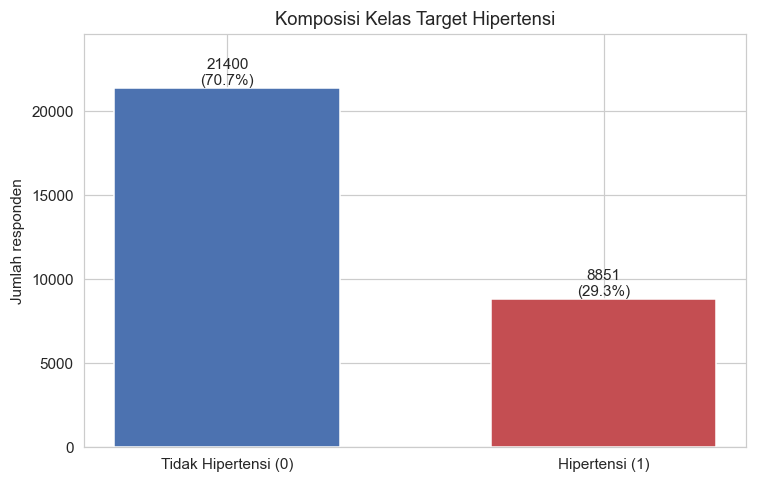
\includegraphics[width=0.6\textwidth]{images/eda/g1_target_balance.png}
    \caption{Komposisi Kelas Target Hipertensi}
    \label{fig:komposisi-kelas-target}
\end{figure}
 
Gambar~\ref{fig:komposisi-kelas-target} menyajikan komposisi kelas pada variabel target setelah proses pelabelan dilakukan. Dari 30.251 responden dewasa, sebanyak 8.851 orang atau 29,26\% tergolong hipertensi, sedangkan 21.400 orang atau 70,74\% tidak hipertensi. Rasio antara kedua kelas sekitar satu berbanding dua koma empat, yang tergolong relatif seimbang dan jauh lebih baik dibandingkan apabila diabetes dijadikan target dengan kasus positif kurang dari satu persen. Oleh karena itu, pemodelan dapat dilakukan tanpa teknik penyeimbangan kelas yang agresif, meskipun metrik recall dan F1-score tetap perlu dipantau di samping akurasi.
 
\begin{figure}[htbp]
    \centering
    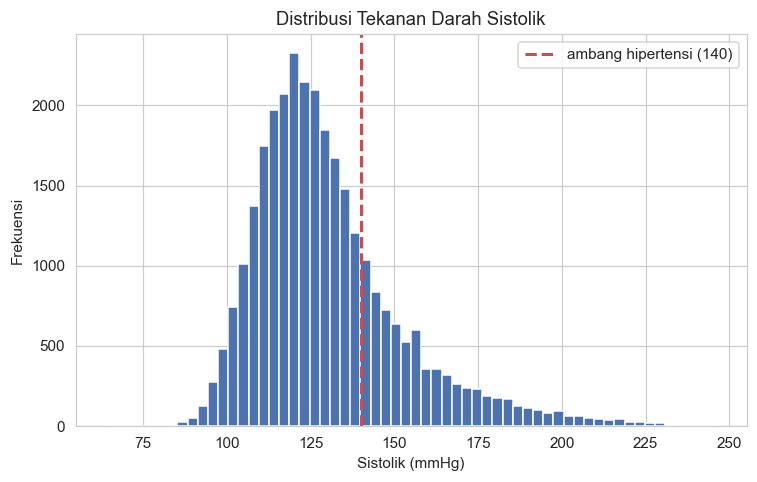
\includegraphics[width=0.6\textwidth]{images/eda/g2_systolic.png}
    \caption{Distribusi Tekanan Darah Sistolik}
    \label{fig:distribusi-sistolik}
\end{figure}
 
Gambar~\ref{fig:distribusi-sistolik} memperlihatkan sebaran tekanan darah sistolik beserta garis ambang 140 mmHg. Distribusi memuncak pada kisaran 110 sampai 130 mmHg dan cenderung menjulur ke kanan hingga melewati 200 mmHg. Sebagian responden berada di sebelah kanan garis ambang, dan kelompok inilah yang tergolong hipertensi dari sisi sistolik. Kemiringan distribusi ke kanan menandakan adanya sejumlah nilai pencilan pada sisi tinggi yang perlu ditangani dengan hati-hati pada tahap berikutnya.
 
\begin{figure}[htbp]
    \centering
    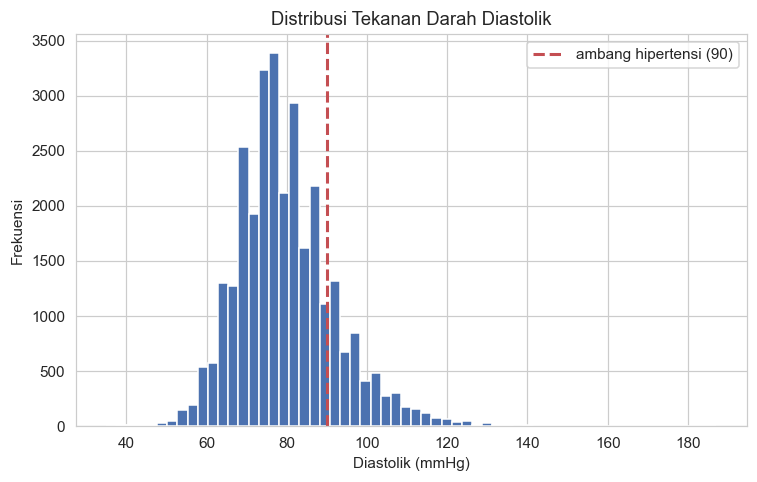
\includegraphics[width=0.6\textwidth]{images/eda/g3_diastolic.png}
    \caption{Distribusi Tekanan Darah Diastolik}
    \label{fig:distribusi-diastolik}
\end{figure}
 
Gambar~\ref{fig:distribusi-diastolik} menampilkan sebaran tekanan darah diastolik beserta garis ambang 90 mmHg. Distribusi diastolik terlihat lebih simetris dibandingkan sistolik, dengan puncak pada kisaran 70 sampai 85 mmHg. Seorang responden dapat tergolong hipertensi melalui kriteria diastolik meskipun nilai sistoliknya masih di bawah 140 mmHg, karena pelabelan cukup memenuhi salah satu dari kedua kriteria tersebut. Dengan demikian, kedua komponen tekanan darah sama-sama berperan dalam pembentukan label.
 
\begin{figure}[htbp]
    \centering
    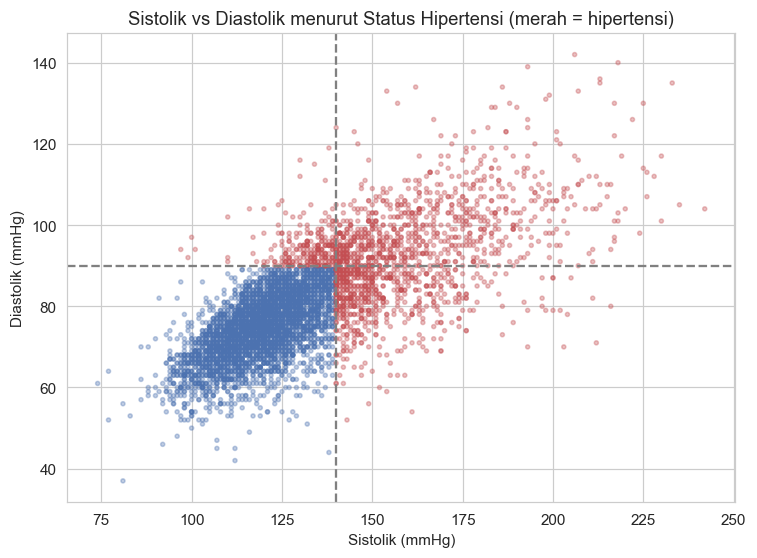
\includegraphics[width=0.7\textwidth]{images/eda/g4_scatter.png}
    \caption{Sistolik vs Diastolik menurut Status Hipertensi}
    \label{fig:sistolik-vs-diastolik}
\end{figure}
 
Gambar~\ref{fig:sistolik-vs-diastolik} menggabungkan tekanan sistolik pada sumbu horizontal dan diastolik pada sumbu vertikal, dengan warna merah menandai responden hipertensi. Titik berwarna merah mengelompok di sebelah kanan garis 140 dan di atas garis 90, sedangkan titik berwarna biru terkonsentrasi pada pojok kiri bawah. Pemisahan yang tampak jelas ini terjadi karena label memang dihitung langsung dari kedua nilai tekanan darah. Hal ini menjadi peringatan penting, sebab memasukkan tekanan darah sebagai fitur akan menimbulkan kebocoran data, sehingga kedua variabel tersebut wajib dikeluarkan dari daftar prediktor.
 
\subsubsection{Kelengkapan Data dan Statistik Deskriptif}
 
Permasalahan kualitas data yang paling menonjol adalah tingginya proporsi nilai hilang yang tersebar tidak merata antarvariabel. Sebagian kolom hampir kosong, sementara sebagian lain hampir lengkap. Tabel~\ref{tab:missing-value-grouping} mengelompokkan variabel menurut tingkat kekosongannya agar strategi penanganannya dapat ditentukan secara proporsional. Pengelompokan ini penting karena kolom dengan kekosongan parah memerlukan perlakuan yang berbeda dari kolom dengan kekosongan ringan.
 
\begin{table}[H]
    \centering
    \caption{Pengelompokan Variabel Berdasarkan Tingkat Nilai Hilang}
    \label{tab:missing-value-grouping}
    \begin{tabular}{@{}p{2.3cm} p{2.6cm} p{8.3cm}@{}}
        \toprule
        \textbf{Kategori} & \textbf{Rentang Hilang} & \textbf{Variabel} \\
        \midrule

        Sangat parah & 50\% ke atas &
        \textit{freq\_fast\_food} 90,4\%, \textit{freq\_soda} 83,2\%, \textit{freq\_hard\_act} 81,0\%, \textit{waist\_cm} 63,7\%, \textit{freq\_moderate\_act} 51,7\% \\[4pt]

        Sedang & 10\% sampai 50\% &
        \textit{freq\_fried\_food} 43,8\%, \textit{freq\_walking} 39,7\%, \textit{sleep\_disturbance} 13,6\%, \textit{sleep\_quality} 13,6\%, \textit{bp\_systolic} dan \textit{bp\_diastolic} 10,6\%, \textit{weight\_kg} 10,4\%, \textit{height\_cm} 10,3\% \\[4pt]

        Ringan & di bawah 10\% &
        \textit{is\_diabetes} 5,9\%, \textit{is\_high\_cholesterol} 5,9\%, \textit{is\_smoking} 5,8\%, \textit{age} 0,03\%, \textit{sex} 0,02\% \\[4pt]

        Lengkap & sekitar 0\% &
        \textit{pidlink} \\

        \bottomrule
    \end{tabular}

    \vspace{2mm}

\end{table}
 
Untuk memperjelas sebaran kekosongan tersebut, proporsi nilai hilang setiap kolom divisualisasikan pada Gambar~\ref{fig:missing-value}. Grafik tersebut memperlihatkan bahwa kelompok variabel gaya hidup, yaitu frekuensi konsumsi makanan dan aktivitas fisik, mendominasi sisi kiri dengan kekosongan tertinggi. Sebaliknya, variabel identitas dan demografi seperti \textit{pidlink}, \textit{sex}, dan \textit{age} berada pada sisi kanan dengan kekosongan mendekati nol. Visualisasi ini mempertegas bahwa keputusan seleksi fitur nantinya perlu mempertimbangkan tingkat kelengkapan tiap variabel.
 
\begin{figure}[htbp]
    \centering
    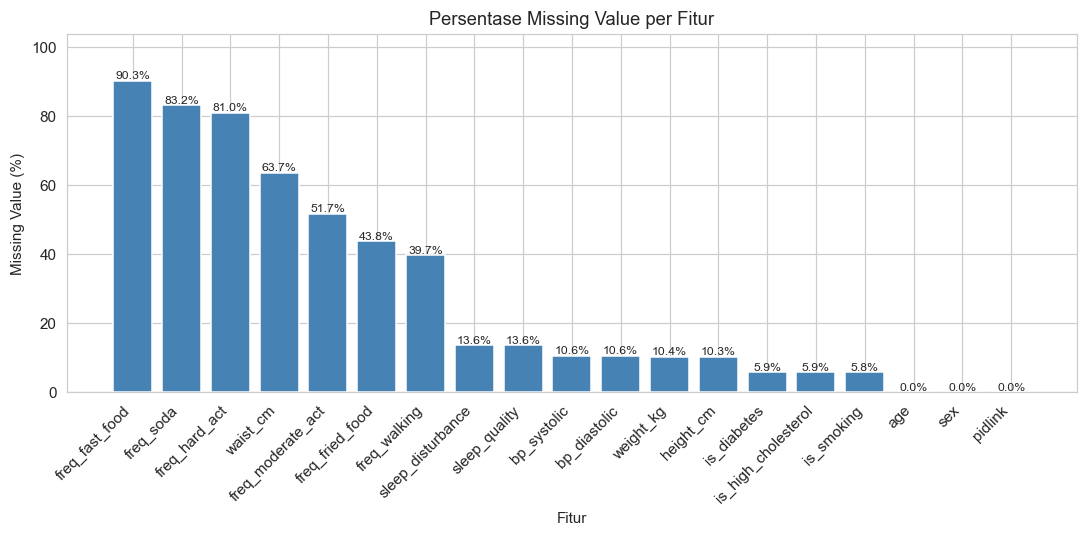
\includegraphics[width=0.9\textwidth]{images/eda/missing_values.png}
    \caption{Persentase Missing Value per Fitur}
    \label{fig:missing-value}
\end{figure}
 
Pola nilai hilang ini bersifat tidak acak dan tampak mengikuti desain survei. Variabel aktivitas fisik dan pola makan kosong pada sebagian besar responden bukan karena kesalahan pencatatan, melainkan karena pertanyaannya hanya diajukan kepada sebagian peserta. Kekosongan dengan pola seperti ini berisiko menimbulkan bias apabila ditambal secara sembarangan. Oleh karena itu, penanganannya tidak dapat diseragamkan, dan sebagian kolom mungkin lebih baik dibuang daripada dipaksakan untuk dipertahankan.
 
Statistik deskriptif digunakan untuk memahami rentang nilai dan kecenderungan tiap variabel numerik. Karena kolom \textit{bmi} tidak tersedia pada dataset, nilainya dihitung terlebih dahulu dari berat dan tinggi badan sebelum diringkas. Tabel~\ref{tab:statistik-deskriptif} menyajikan tujuh variabel numerik utama beserta ukuran pemusatan dan penyebarannya. Pemeriksaan terhadap nilai ekstrem juga dilakukan untuk mendeteksi kemungkinan kesalahan pencatatan.
 
\begin{table}[htbp]
    \centering
    \caption{Statistik Deskriptif Variabel Numerik}
    \label{tab:statistik-deskriptif}
    \begin{tabular}{@{}lrrrrrr@{}}
        \toprule
        \textbf{Variabel} & \textbf{N} & \textbf{Mean} & \textbf{Std} & \textbf{Min} & \textbf{Median} & \textbf{Maks} \\
        \midrule
        \textit{age}          & 30.251 & 39,95  & 15,21 & 18    & 37    & 110 \\
        \textit{weight\_kg}   & 30.083 & 57,27  & 11,87 & 22,0  & 56,0  & 133,1 \\
        \textit{height\_cm}   & 30.109 & 156,35 & 8,50  & 94,3  & 156,0 & 198,0 \\
        \textit{waist\_cm}    & 13.097 & 83,93  & 11,77 & 32,0  & 83,6  & 150,0 \\
        \textit{bmi}          & 30.055 & 23,42  & 4,45  & 10,85 & 22,82 & 68,76 \\
        \textit{bp\_systolic} & 30.251 & 130,12 & 22,37 & 64    & 126   & 246 \\
        \textit{bp\_diastolic}& 30.251 & 79,82  & 12,37 & 35    & 78    & 187 \\
        \bottomrule
    \end{tabular}
    \\[4pt]
\end{table}
 
Beberapa nilai pada tabel tersebut layak dicermati lebih lanjut. Nilai rata-rata yang konsisten lebih tinggi daripada median pada berat badan, bmi, dan tekanan darah menunjukkan distribusi yang condong ke kanan, yang merupakan ciri umum data antropometri. Nilai maksimum bmi sebesar 68,76 dan sistolik sebesar 246 mengindikasikan keberadaan pencilan pada sisi tinggi. Sementara itu, usia kini berhenti pada angka wajar 110 tahun setelah nilai berkode khusus 998 dibersihkan.
 
\begin{figure}[htbp]
    \centering
    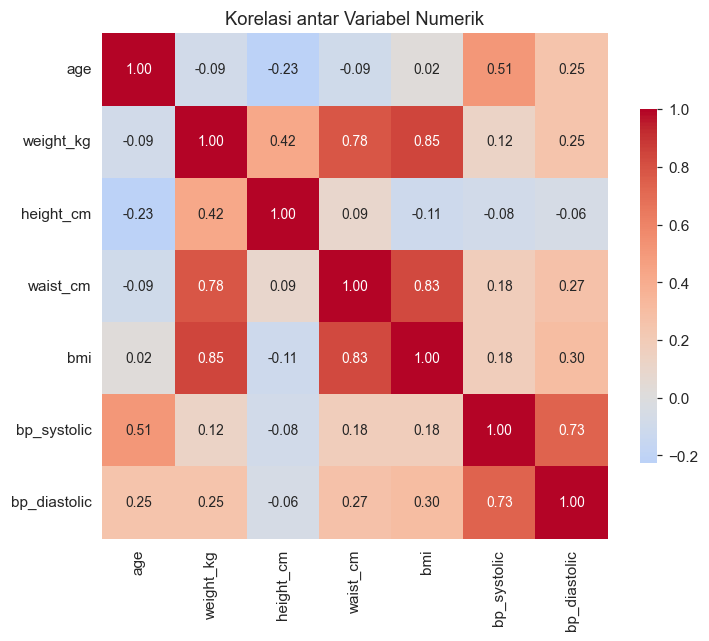
\includegraphics[width=0.55\textwidth]{images/eda/g5_corr.png}
    \caption{Korelasi antar Variabel Numerik}
    \label{fig:korelasi-numerik}
\end{figure}
 
Gambar~\ref{fig:korelasi-numerik} menyajikan matriks korelasi antarvariabel numerik untuk mengidentifikasi keterkaitan dan redundansi. Korelasi tertinggi ditemukan antara bmi dengan berat badan sebesar 0,85 dan dengan lingkar pinggang sebesar 0,83, yang wajar karena ketiganya mengukur dimensi tubuh yang serupa. Tekanan sistolik dan diastolik juga menunjukkan korelasi yang kuat sebesar 0,73. Tingginya korelasi antarvariabel ini menandakan adanya multikolinearitas, sehingga cukup dipilih salah satu variabel sebagai wakil agar model tidak menjadi tidak stabil.
 
\subsubsection{Analisis Bivariat antara Fitur dan Hipertensi}
 
Analisis bivariat dilakukan untuk mengidentifikasi faktor yang paling berhubungan dengan kejadian hipertensi. Secara kuantitatif, analisis menggunakan koefisien korelasi point-biserial untuk mengukur kedekatan hubungan variabel numerik, serta analisis komparatif untuk menghitung tingkat kejadian pada setiap subkelompok. Secara visual, hubungan tersebut direpresentasikan melalui grafik batang dan grafik batang berkelompok untuk mengidentifikasi pola serta perbedaan distribusi persentase hipertensi. Hasil korelasi disajikan pada Tabel~\ref{tab:korelasi-pointbiserial}, yang menunjukkan bahwa hanya sebagian kecil faktor yang berhubungan kuat, sedangkan sebagian besar lainnya berhubungan lemah.
 
\begin{table}[htbp]
    \centering
    \caption{Korelasi Point-Biserial Fitur Numerik dengan Hipertensi}
    \label{tab:korelasi-pointbiserial}
    \begin{tabular}{@{}lr@{}}
        \toprule
        \textbf{Fitur} & \textbf{Korelasi dengan Hipertensi} \\
        \midrule
        \textit{age}                & +0,410 \\
        \textit{bmi}                & +0,186 \\
        \textit{waist\_cm}          & +0,186 \\
        \textit{sleep\_quality}     & +0,060 \\
        \textit{freq\_fried\_food}  & +0,025 \\
        \textit{freq\_moderate\_act}& +0,017 \\
        \textit{freq\_walking}      & +0,011 \\
        \textit{freq\_hard\_act}    & +0,009 \\
        \textit{freq\_fast\_food}   & -0,006 \\
        \textit{freq\_soda}         & -0,009 \\
        \textit{sleep\_disturbance} & -0,032 \\
        \bottomrule
    \end{tabular}
    \\[4pt]

\end{table}
 
\begin{figure}[htbp]
    \centering
    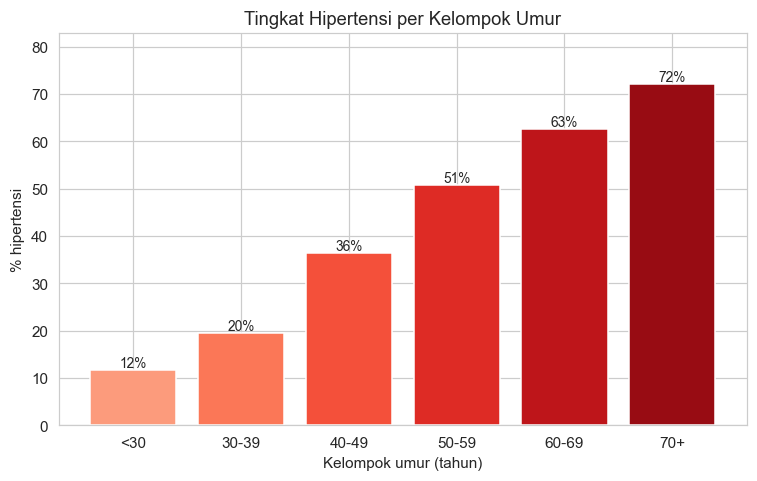
\includegraphics[width=0.6\textwidth]{images/eda/g6_umur.png}
    \caption{Tingkat Hipertensi per Kelompok Umur}
    \label{fig:hipertensi-umur}
\end{figure}
 
Gambar~\ref{fig:hipertensi-umur} menggambarkan tingkat hipertensi pada setiap kelompok umur. Tingkat hipertensi meningkat secara konsisten, mulai dari sekitar 12\% pada kelompok di bawah 30 tahun, lalu 36\% pada rentang 40 sampai 49 tahun, hingga mencapai 72\% pada kelompok 70 tahun ke atas. Tidak terdapat satu pun kelompok yang membalik kecenderungan kenaikan tersebut. Dengan korelasi tertinggi di antara seluruh kandidat sebesar 0,410, usia menjadi faktor risiko paling dominan dan kemungkinan besar menjadi prediktor utama dalam pemodelan.
 
\begin{figure}[htbp]
    \centering
    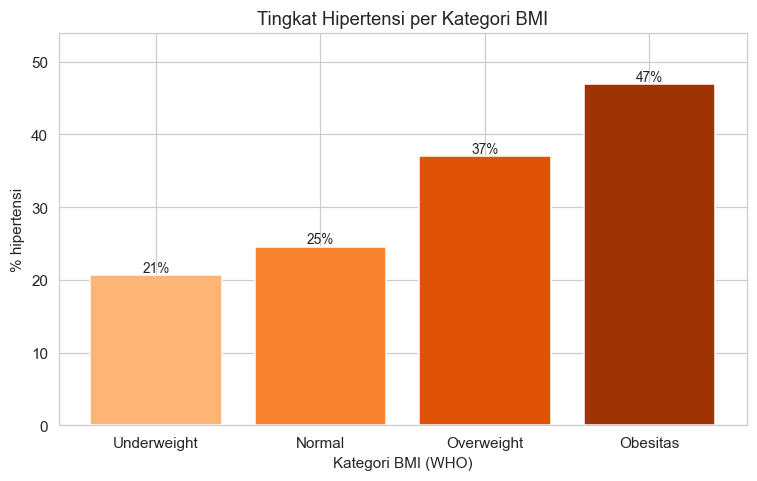
\includegraphics[width=0.6\textwidth]{images/eda/g7_bmi.png}
    \caption{Tingkat Hipertensi per Kategori BMI}
    \label{fig:hipertensi-bmi}
\end{figure}
 
Gambar~\ref{fig:hipertensi-bmi} memperlihatkan tingkat hipertensi menurut kategori indeks massa tubuh berdasarkan klasifikasi WHO. Tingkat hipertensi meningkat seiring naiknya kategori, yaitu 21\% pada kelompok underweight, 25\% pada kelompok normal, 37\% pada kelompok overweight, dan 47\% pada kelompok obesitas. Selisih lebih dari dua kali lipat antara kelompok underweight dan obesitas menunjukkan hubungan positif yang kuat antara kelebihan berat badan dan hipertensi. Karena bmi dihitung sendiri dari berat dan tinggi badan, variabel ini menjadi ringkasan yang menggantikan kedua variabel asalnya sekaligus.
 
Faktor gaya hidup lain menunjukkan hubungan yang lemah dengan hipertensi. Frekuensi aktivitas fisik dan pola makan, yaitu aktivitas berat, sedang, jalan kaki, fast food, soda, dan gorengan, seluruhnya hanya memiliki korelasi yang sangat kecil, di bawah nol koma nol tiga, sebagian bahkan bernilai negatif. Nilai korelasi yang sangat kecil tersebut diperberat oleh kekosongan data yang tinggi, yaitu 91\% pada fast food, 84\% pada soda, dan 81\% pada aktivitas berat. Dengan kondisi tersebut, variabel-variabel gaya hidup ini menjadi kandidat paling lemah dan berpotensi dibuang pada tahap seleksi fitur.
 
\begin{figure}[htbp]
    \centering
    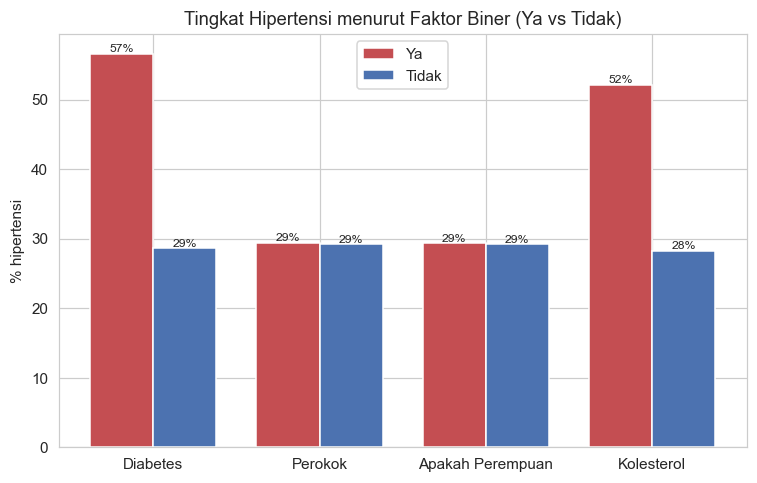
\includegraphics[width=0.6\textwidth]{images/eda/g8_biner.png}
    \caption{Tingkat Hipertensi menurut Faktor Biner}
    \label{fig:hipertensi-biner}
\end{figure}
 
Gambar~\ref{fig:hipertensi-biner} membandingkan tingkat hipertensi antara kelompok yang memiliki dan tidak memiliki suatu karakteristik pada empat faktor biner. Dua faktor menonjol tajam, yaitu status diabetes dengan tingkat hipertensi 56,6\% berbanding 28,6\%, serta status kolesterol tinggi dengan tingkat 52,1\% berbanding 28,2\%. Sebaliknya, kebiasaan merokok hanya menghasilkan selisih sekitar 0,3\% dan jenis kelamin nyaris tidak menunjukkan perbedaan. Perlu dicatat bahwa sebagian hubungan diabetes dan kolesterol dengan hipertensi dapat dipengaruhi oleh faktor usia, karena ketiga kondisi tersebut cenderung meningkat pada kelompok yang lebih tua.
 
\begin{figure}[htbp]
    \centering
    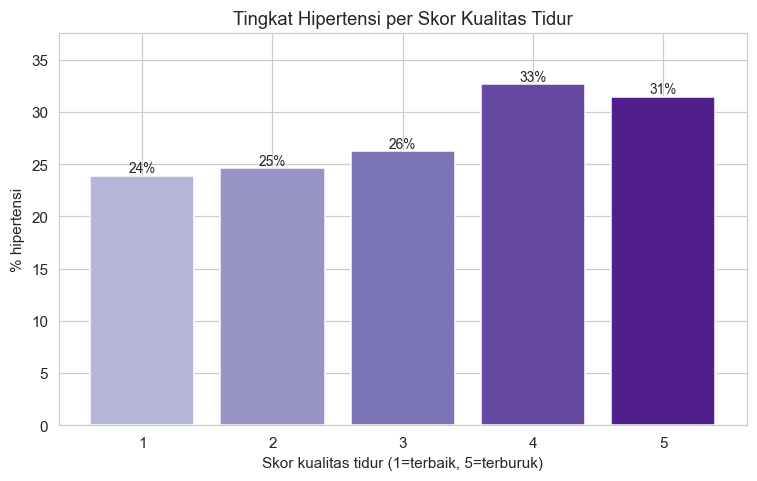
\includegraphics[width=0.6\textwidth]{images/eda/g9_sleep.png}
    \caption{Tingkat Hipertensi per Skor Kualitas Tidur}
    \label{fig:hipertensi-tidur}
\end{figure}
 
Gambar~\ref{fig:hipertensi-tidur} menampilkan tingkat hipertensi menurut skor kualitas tidur. Terdapat kecenderungan kenaikan yang landai, dari sekitar 24\% pada skor terbaik hingga sekitar 32\% pada saat kualitas tidur memburuk. Korelasinya tergolong kecil, yaitu 0,06, sehingga fitur ini bukan merupakan faktor utama. Meskipun demikian, arah hubungannya masuk akal secara klinis dan datanya cukup lengkap, sehingga fitur ini masih layak dipertahankan sebagai faktor pendukung.
 
\subsubsection{Karakteristik yang Memengaruhi Pemodelan}
 
Beberapa hasil eksplorasi berdampak langsung pada perancangan model. Yang pertama dan paling penting, tekanan darah harus dikeluarkan dari daftar fitur, karena label hipertensi dibentuk langsung dari sistolik dan diastolik sehingga penyertaannya akan menimbulkan kebocoran data. Yang kedua, komposisi target yang relatif seimbang pada 29,26\% memungkinkan penggunaan pendekatan standar tanpa penyeimbangan kelas yang agresif, meskipun metrik recall dan F1-score tetap perlu dipantau. Yang ketiga, analisis bivariat menunjukkan bahwa usia, bmi, status diabetes, dan status kolesterol tinggi merupakan kandidat fitur terkuat, sedangkan aktivitas fisik, pola makan, dan lingkar pinggang yang sarat kekosongan layak dipertimbangkan untuk dibuang, dengan kualitas tidur sebagai faktor pendukung yang lemah namun masih dapat dipertahankan.
 
\subsubsection{Identifikasi Anomali dan Permasalahan Data}
 
Pemeriksaan terhadap nilai ekstrem dan kualitas data mengungkap beberapa permasalahan yang harus ditangani pada tahap persiapan data, yaitu sebagai berikut.
 
\begin{enumerate}
    \item Nilai berkode khusus pada variabel \textit{age} \\
    Nilai 998 muncul pada empat baris dan teridentifikasi sebagai kode nilai hilang, sebab usia valid tertinggi berikutnya adalah 110 tahun. Apabila tidak dikonversi menjadi nilai hilang, kode ini akan mendistorsi seluruh statistik dan korelasi terkait usia.
 
    \item Nilai tekanan darah yang mustahil secara fisiologis \\
    Ditemukan tiga baris dengan nilai diastolik lebih besar atau sama dengan sistolik serta nilai di luar rentang wajar yang mengindikasikan kesalahan pencatatan.
 
    \item Ketidaksesuaian tipe data \\
    Variabel kategorik berkode terbaca sebagai numerik dan perlu dikonversi serta dipetakan ulang dari kode 1/3 menjadi representasi biner 1/0 agar interpretasi model lebih jelas.
 
    \item Nilai hilang \\
    Sejumlah kolom gaya hidup memiliki proporsi nilai hilang yang sangat tinggi, mencapai 90\% pada fast food, sehingga tidak dapat diimputasi secara wajar dan menjadi kandidat untuk dibuang pada tahap seleksi fitur.
\end{enumerate}
 
 
Dataset ini masih menyimpan sejumlah permasalahan kualitas data pada isinya. Permasalahan tersebut meliputi nilai berkode khusus, nilai tekanan darah yang mustahil, serta nilai hilang yang tidak acak dengan proporsi tinggi pada variabel gaya hidup. Analisis menunjukkan sinyal yang cukup jelas, yaitu hipertensi paling kuat berhubungan dengan usia dan berat badan, dengan status diabetes dan kolesterol tinggi sebagai faktor penegas. Seluruh temuan ini menjadi dasar dalam merancang tahap persiapan data pada subbab berikutnya.


% \subsubsection{Hasil Integrasi Data Mentah}
% Hasil akhir dari proses integrasi menghasilkan sebuah dataset mentah tunggal dengan 36.391 baris responden dan seluruh kolom fitur yang dibutuhkan. Pemeriksaan awal menunjukkan bahwa dataset ini secara teknis belum siap untuk pemodelan karena mengandung beberapa masalah kualitas data yang memerlukan penanganan, antara lain:



% \begin{enumerate}
% \item Nilai yang hilang\\
% Sejumlah kolom yang mengandung NaN baik akibat ketidakhadiran responden pada modul tertentu maupun jawaban `tidak tahu' atau penolakan menjawab.

% \item Kode kategoris non-standar\\
% Beberapa variabel menggunakan sistem pengkodean spesifik IFLS yang tidak kompatibel langsung dengan algoritma \textit{machine learning}, seperti kode 1/3 untuk ya/tidak, bukan 1/0, dan kode alfanumerik pada variabel kesehatan orang tua.

% \item Kode sentinel\\
% Pada variabel diabetes, kode 8 digunakan untuk `Tidak Tahu' dan kode 9 untuk `Tidak Menjawab/Data Hilang', yang perlu dibedakan dari nilai 1 (Ya) dan 3 (Tidak) yang valid.

% \item Representasi teks pada variabel kategoris\\
% Kolom riwayat kesehatan orang tua menggunakan kode huruf kombinasi, contohnya seperti A, B, BCD, BD, yang memerlukan rekayasa fitur untuk mengubahnya menjadi representasi numerik yang bermakna.
% \end{enumerate}


% Kapasitas memori perangkat cukup terbatas sehingga peneliti tidak memuat semua kolom sekaligus. 
% Peneliti hanya mengekstrak kolom yang relevan dengan faktor risiko hipertensi dari setiap berkas. 
% Proses ekstraksi ini menggunakan pustaka \textit{pyreadstat} pada bahasa pemrograman \textit{Python}. 
% Peneliti kemudian menggabungkan hasil ekstraksi tersebut berdasarkan \textit{pidlink}.

% Penelitian ini menargetkan 10 faktor risiko. 
% Tabel V.1 merangkum status ketersediaan setiap faktor risiko pada dataset akhir bernama \textit{master\_dataset\_raw\_final.csv}.

% \begin{table}[htbp]
%     \centering
%     \caption{Status ketersediaan faktor risiko pada dataset akhir}
%     \vspace{0.5em}
%     \begin{tabular}{clll}
%         \toprule
%         \textbf{No.} & \textbf{Faktor Risiko} & \textbf{Status} & \textbf{Variabel} \\
%         \midrule
%         1 & Usia & Tersedia & \textit{age} \\
%         2 & Jenis kelamin & Tersedia & \textit{sex} \\
%         3 & Riwayat orang tua & Tidak tersedia & \textit{father\_health}, \textit{mother\_health} \\
%         4 & Indeks massa tubuh & Tidak tersedia & \textit{weight\_kg}, \textit{height\_cm} \\
%         5 & Makanan asin/mi instan & Tersedia (90\% kosong) & \textit{freq\_instant\_noodle} \\
%         6 & Aktivitas fisik & Tersedia & \textit{ak02}, \textit{ak05}, \textit{ak07} \\
%         7 & Merokok & Tersedia & \textit{km01a}, \textit{km04} \\
%         8 & Lingkar pinggang & Tersedia & \textit{waist\_cm} \\
%         9 & Diabetes & Tersedia (309 kasus positif) & \textit{is\_diabetes} \\
%         10 & Stres & Tersedia & \textit{ps\_A} s.d. \textit{ps\_F} \\
%         \bottomrule
%     \end{tabular}
% \end{table}

% Peneliti berhasil memperoleh tujuh dari 10 faktor risiko target pada tahap ini. Dua faktor belum tersedia, yaitu riwayat kesehatan orang tua dan indeks massa tubuh. Peneliti belum mendapatkan kedua faktor ini karena gagal mengekstrak kolom terkait dari \textit{Book US} dan modul BA. 
% Variabel makanan asin memang tersedia, tetapi 90 persen nilainya kosong sehingga kegunaan variabel ini menjadi terbatas. 
% Variabel target meliputi tekanan darah sistolik (\textit{bp\_systolic}) dan diastolik (\textit{bp\_diastolic}). 
% Variabel target ini sudah tersedia. 
% Namun, peneliti menemukan anomali nilai pada variabel target ini. 
% Peneliti perlu menangani anomali tersebut pada tahap penyiapan data.


% \subsection{Eksplorasi Data Awal}

% Setelah proses akuisisi dan penggabungan data selesai dilakukan, tahap berikutnya adalah eksplorasi data awal untuk memahami karakteristik dataset yang akan digunakan. Tahap ini bertujuan untuk mengidentifikasi struktur data, mengetahui persebaran nilai pada setiap variabel, menemukan pola-pola yang muncul, serta mendeteksi karakteristik data yang berpotensi memengaruhi proses prapemrosesan dan pembangunan model. Eksplorasi dilakukan melalui pemeriksaan isi dataset, analisis statistik deskriptif, serta penyajian data dalam bentuk visualisasi guna memperoleh gambaran awal mengenai kondisi dan kualitas data yang tersedia.




% \subsubsection{Eksplorasi Data Awal}

% \section{\emph{Data Preparation}}
% Tahap persiapan data mencakup serangkaian proses transformasi dan pembersihan yang diperlukan sebelum data dapat digunakan untuk melatih model \textit{machine learning}. Pembersihan data merupakan proses paling kritis dalam keseluruhan alur kerja penelitian ini. Kualitas data yang bersih secara langsung memengaruhi keandalan dan validitas model prediktif yang akan dibangun. Proses pembersihan dilaksanakan dalam satu skrip terpusat yang dieksekusi sehingga dapat direplikasi kapan pun dengan hasil yang identik.

% \subsection{Penghapusan Baris dengan Nilai Hilang pada Variabel Kritis}

% Langkah pertama pada tahap pembersihan data adalah menghapus seluruh baris yang memiliki nilai hilang pada variabel \textit{bp\_systolic}, \textit{bp\_diastolic}, dan \textit{bmi}. Ketiga variabel tersebut dikategorikan sebagai variabel kritis karena memiliki peran penting dalam penelitian. Variabel \textit{bp\_systolic} dan \textit{bp\_diastolic} digunakan sebagai dasar pembentukan label target hipertensi, sehingga ketiadaan salah satu atau kedua variabel tersebut menyebabkan status hipertensi responden tidak dapat ditentukan. Sementara itu, variabel \textit{bmi} merupakan salah satu prediktor utama yang secara klinis memiliki hubungan erat dengan hipertensi. Oleh karena itu, nilai hilang pada variabel ini tidak diimputasi karena berpotensi memperkenalkan bias yang dapat memengaruhi kualitas hasil analisis dan pemodelan.

% Strategi penghapusan baris dipilih atas pertimbangan bahwa data tanpa variabel kritis ini sepenuhnya tidak dapat digunakan untuk tujuan penelitian, baik sebagai data latih maupun data uji. Jika penulis ingin melakukan imputasi nilai tekanan darah, misalnya dengan nilai rata-rata, akan tercipta label hipertensi sintetis yang tidak mencerminkan kondisi medis nyata responden dan berpotensi mengganggu seluruh analisis. Proses ini menghasilkan penyisutan populasi dari 36.391 menjadi 32.334 responden, menghasilkan tingkat retensi sebesar 88,9\%.

% \subsection{Imputasi Nilai Kosong}

% Berbeda dengan variabel kritis, nilai yang hilang pada variabel-variabel yang merepresentasikan perilaku atau kegiatan sehari-hari tidak diinterpretasikan sebagai data yang benar-benar hilang, melainkan sebagai indikasi bahwa responden tidak melakukan kegiatan yang ditanyakan. Oleh karena itu, imputasi nol diterapkan pada variabel-variabel berikut.

% \begin{enumerate}
% \item Frekuensi konsumsi mie instan\\
% Pada fitur frekuensi konsumsi mie instan yang mencakup \textit{freq\_instant\_noodle}, Responden yang tidak memberikan jawaban diasumsikan tidak mengonsumsi mie instan. Nilai NaN diisi dengan 0 (kali per minggu).

% \item Aktivitas fisik\\
% Pada fitur aktivitas fisik yang mencakup \textit{ak02}, \textit{ak05}, \textit{ak07}, Responden yang tidak menjawab pertanyaan tentang frekuensi aktivitas fisik diasumsikan tidak berolahraga atau berjalan kaki secara teratur dalam minggu survei. Nilai NaN diisi dengan 0 (hari per minggu).
% \end{enumerate}

% Pendekatan ini konsisten dengan panduan imputasi pada data survei perilaku kesehatan, yang mengasumsikan bahwa ketidakhadiran jawaban pada pertanyaan tentang kegiatan tertentu lebih mungkin bermakna `tidak melakukan' daripada `lupa menjawab', terutama apabila pertanyaan tersebut bersifat spesifik dan mudah diingat oleh responden.

% \subsection{Penanganan Kode Kategoris}

% Sistem pengkodean variabel kategoris dalam IFLS tidak secara langsung kompatibel dengan representasi yang dibutuhkan oleh algoritma \textit{machine learning}. Tiga variabel utama memerlukan transformasi pengkodean (\textit{re-encoding}) sebagai berikut.

% \begin{enumerate}
% \item Variabel Merokok \\
% Variabel merokok yang direpresentasikan di IFLS dalam \textit{km01a} menggunakan kode 1 untuk `Ya' (pernah merokok) dan kode 3 untuk `Tidak'. Nilai NaN terlebih dahulu diisi dengan kode 3 (Tidak) berdasarkan asumsi yang sama seperti pada variabel perilaku lainnya. Selanjutnya, penulis mebentuk variabel baru dengan nama \textit{is\_smoker}, Pada variabel ini, kode 1 diubah menjadi nilai 1 dan seluruh nilai lainnya menjadi 0.

% \item Variabel Diabetes \\
% Variabel diabetes yang direpresentasikan di IFLS dalam \textit{is\_diabetes} memiliki empat kemungkinan nilai: 1 (Ya/pernah didiagnosis), 3 (Tidak), 8 (Tidak tahu), dan 9 (Tidak menjawab atau data hilang). Kode sentinel 8 dan 9 terlebih dahulu diubah menjadi kode 3 (Tidak) menggunakan operasi \textit{replace}, dengan argumen bahwa responden yang tidak mengetahui status diabetesnya atau menolak menjawab tidak memiliki riwayat diagnosis klinis yang terdokumentasi. Variabel biner \textit{has\_diabetes} kemudian dibentuk dengan nilai 1 apabila kode asli adalah 1 dan 0 untuk kode lainnya.

% \item Variabel Jenis Kelamin \\
% Variabel jenis kelamin yang direpresentasikan di IFLS dalam \textit{sex} menggunakan kode 1 untuk laki-laki dan kode 3 untuk perempuan (bukan kode 2 sebagaimana konvensi umum). Variabel biner \textit{is\_female} dibentuk dengan nilai 1 untuk kode 3 (perempuan) dan nilai 0 untuk kode lainnya. Transformasi ini juga mengeliminasi ambiguitas kode yang tidak standar sebelum data dimasukkan ke dalam model.

% \end{enumerate}

% \subsection{Rekayasa Fitur Riwayat Kesehatan Orang Tua}

% Variabel \textit{father\_health} dan \textit{mother\_health} dari IFLS-4 menyimpan informasi kondisi kesehatan orang tua dalam format kode alfanumerik yang kompleks. Kode-kode ini dapat berupa huruf tunggal maupun kombinasi beberapa huruf, dengan setiap huruf merepresentasikan kondisi tertentu:
% \begin{itemize}
%     \item Kode A: Sehat (masih hidup dan tidak memiliki penyakit yang dilaporkan)
%     \item Kode B: Penyakit jantung atau pembuluh darah
%     \item Kode C: Penyakit paru-paru
%     \item Kode D: Diabetes melitus
%     \item Kode kombinasi (contoh: BCD, BD): Orang tua memiliki lebih dari satu kondisi atau telah meninggal dengan riwayat penyakit tertentu
% \end{itemize}

% Untuk mengubah representasi ini menjadi fitur numerik yang dapat digunakan model, dirancang sebuah fungsi rekayasa fitur dengan logika sebagai berikut: apabila nilai adalah NaN atau berisi huruf `A' saja (tanpa huruf lain), maka orang tua yang bersangkutan dikategorikan sebagai tidak berisiko atau bernilai 0. Apabila nilai mengandung huruf selain A atau merupakan kombinasi huruf, maka orang tua dikategorikan sebagai berisiko atau bernilai 1. Logika ini diterapkan secara terpisah pada kolom \textit{father\_health} menghasilkan \textit{risk\_father}, dan pada kolom \textit{mother\_health} menghasilkan \textit{risk\_mother}.

% Kedua kolom biner tersebut kemudian dijumlahkan untuk menghasilkan satu kolom baru bernama \textit{genetic\_risk\_score} dengan rentang nilai ordinal 0 hingga 2: nilai 0 berarti tidak ada orang tua yang memiliki riwayat penyakit, nilai 1 berarti satu orang tua berisiko, dan nilai 2 berarti kedua orang tua berisiko. Representasi ordinal ini dipilih untuk mempertahankan informasi tentang derajat risiko genetik sekaligus menyederhanakan dua variabel menjadi satu, sehingga mengurangi dimensi fitur tanpa kehilangan informasi substantif.
 
% \subsection{Pembentukan Label Target Hipertensi}
 
% Label target biner untuk klasifikasi hipertensi dibentuk berdasarkan kriteria diagnostik yang ditetapkan oleh Joint National Committee ke-7 dan World Health Organization. Menurut panduan ini, seseorang dikategorikan mengalami hipertensi apabila memenuhi setidaknya salah satu dari dua kondisi berikut: tekanan darah sistolik $\geq$ 140 mmHg atau tekanan darah diastolik $\geq$ 90 mmHg.
 
 

% \setlength{\parskip}{1em} 
% \subsection{Penanganan \emph{Missing Value}}
% Inspeksi \emph{missing value} pada dataset mengungkap dua kelompok fitur yang memerlukan penanganan khusus. Pertama, fitur \textit{waist\_cm} (lingkar pinggang) memiliki 19.300 nilai kosong atau setara dengan 59,7\% dari total data. Meskipun persentase \emph{missing} yang tinggi ini sempat mempertimbangkan opsi penghapusan kolom, fitur ini dipertahankan mengingat relevansinya yang signifikan sebagai indikator klinis risiko hipertensi. Imputasi dilakukan menggunakan nilai median sebesar 83,6 cm, yang lebih kuat terhadap distribusi data yang miring dibandingkan nilai rata-rata.

% Kedua, fitur psikososial \textit{ps\_A}, \textit{ps\_B}, \textit{ps\_C}, \textit{ps\_E}, dan \textit{ps\_F} masing-masing memiliki 1.465 nilai kosong atau sebesar 4,5\%. Fitur-fitur ini memiliki skala ordinal 1 hingga 3, sehingga pengisian dengan nilai 0 yang diterapkan pada versi sebelumnya merupakan nilai di luar rentang skala yang valid dan berpotensi mengintroduksi \emph{noise} pada model. Oleh karena itu, imputasi dilakukan menggunakan median masing-masing kolom.

% \subsection{Konversi Tipe Data}
% Fitur \textit{ak05} ditemukan bertipe \emph{object} (\emph{string}) pada dataset asli, yang menyebabkan fitur ini secara otomatis tereksklusi dari proses pemodelan pada implementasi sebelumnya. Konversi ke tipe numerik menggunakan \textit{pd.to\_numeric(errors='coerce')} dilakukan untuk mengikutsertakan fitur ini, sehingga jumlah fitur aktif meningkat dari 15 menjadi 16 variabel.





% \subsection{Normalisasi Data}
% Normalisasi data menggunakan \textit{StandardScaler} diterapkan secara selektif. Logistic Regression yang sensitif terhadap skala fitur menerima data yang telah dinormalisasi melalui mekanisme \emph{pipeline} dari sklearn. Sementara itu, model berbasis pohon keputusan seperti XGBoost tidak memerlukan normalisasi karena proses pembuatan percabangan pada algoritma tersebut didasarkan pada urutan peringkat nilai, bukan besar absolut nilainya. Penerapan normalisasi pada model berbasis pohon pada implementasi sebelumnya telah diperbaiki pada versi ini.





\section{Data Preparation}

Tahap data preparation bertujuan mengubah data mentah menjadi dataset yang bersih, konsisten, dan siap digunakan untuk pemodelan. Seluruh keputusan pada tahap ini dirancang berdasarkan temuan yang diperoleh pada tahap eksplorasi data awal, sehingga setiap permasalahan kualitas data yang teridentifikasi memiliki penanganan yang spesifik. Tahapan ini dilaksanakan menurut urutan yang ketat, sebab setiap langkah memengaruhi langkah berikutnya, terutama yang berkaitan dengan pembentukan label target dan pencegahan kebocoran data. Gambaran umum keseluruhan alur proses data preparation yang diterapkan disajikan pada Gambar \ref{fig:alur_data_prep}.

\begin{figure}[htbp]
    \centering
    % Silakan ganti 'gambar_1_9.png' dengan nama file gambar Anda
    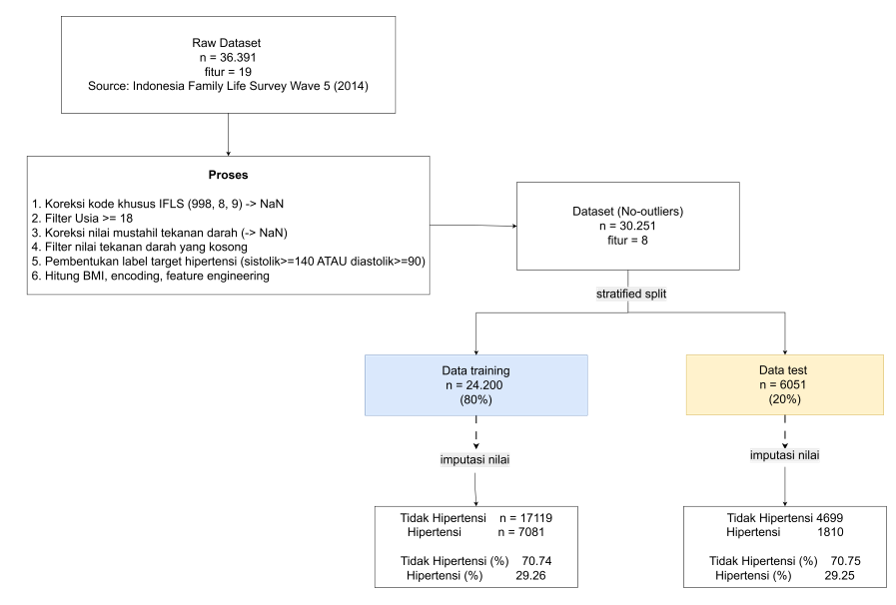
\includegraphics[width=0.75\textwidth]{images/Picture1.png} 
    \caption{Alur Proses Data Preparation}
    \label{fig:alur_data_prep}
\end{figure}

Gambar \ref{fig:alur_data_prep} memperlihatkan gambaran umum alur data preparation, mulai dari dataset mentah (36.391 responden, 19 fitur), melewati serangkaian proses pembersihan dan transformasi, hingga terbentuk dataset bersih tanpa pencilan (30.251 responden, 8 fitur) yang kemudian dibagi secara \emph{stratified} menjadi data latih dan data uji sebelum diimputasi. Rincian proses tersebut dijabarkan ke dalam delapan langkah berurutan (A--H) pada uraian berikut. Penyesuaian utama meliputi penempatan pembersihan kode tersamar di posisi paling awal, penambahan filter usia dewasa, serta penghapusan tekanan darah dari himpunan fitur untuk mencegah kebocoran data. Berbeda dengan rancangan sebelumnya, pembagian data dan imputasi kini dilaksanakan langsung pada tahap ini, dengan imputasi yang hanya dipelajari dari data latih agar tidak terjadi kebocoran informasi. Keseluruhan langkah persiapan data tersebut diringkas dalam bentuk pseudocode pada Algoritma~\ref{alg:data-prep}.

\begin{algorithm}[htbp]
\caption{Prapemrosesan dan Persiapan Data Hipertensi}
\label{alg:data-prep}
\begin{algorithmic}[1]
\Require Dataset mentah IFLS $D$ (36.391 baris, 19 variabel)
\Ensure Data latih $D_{\mathit{train}}$ dan data uji $D_{\mathit{test}}$ (8 fitur $+$ 1 target)
\State Ganti seluruh kode khusus IFLS (8, 9, 998, dan sejenisnya) menjadi nilai kosong \Comment{Langkah A}
\State Buang responden berusia di bawah 18 tahun \Comment{Langkah B}
\State Ubah nilai tekanan darah mustahil menjadi kosong, lalu buang baris tanpa tekanan darah valid \Comment{Langkah C}
\State Bentuk label $y \gets 1$ bila sistolik $\geq 140$ atau diastolik $\geq 90$; selain itu $y \gets 0$ \Comment{Langkah D}
\State Keluarkan \textit{bp\_systolic} dan \textit{bp\_diastolic} dari himpunan fitur \Comment{Langkah E}
\State Kodekan variabel kategorik menjadi representasi biner \Comment{Langkah F}
\State Hitung \textit{bmi} dari berat dan tinggi badan
\ForAll{fitur $f$}
    \If{proporsi nilai hilang $(f) > 30\%$ \textbf{atau} $f$ redundan terhadap \textit{bmi}}
        \State Buang $f$ dari himpunan fitur
    \EndIf
\EndFor \Comment{Langkah G: menyisakan 8 fitur}
\State Bagi $D$ secara \emph{stratified} 80:20 menjadi $D_{\mathit{train}}$ dan $D_{\mathit{test}}$ \Comment{Langkah H}
\State Pelajari nilai imputasi (median untuk numerik/ordinal, modus untuk biner) dari $D_{\mathit{train}}$
\State Terapkan nilai imputasi tersebut ke $D_{\mathit{train}}$ dan $D_{\mathit{test}}$
\State \Return $D_{\mathit{train}}, D_{\mathit{test}}$
\end{algorithmic}
\end{algorithm}

\subsubsection*{A. Pembersihan Nilai Khusus IFLS}
Langkah pertama adalah mengonversi seluruh nilai yang memiliki makna khusus dalam IFLS menjadi nilai kosong. Saat mengisi kuesioner IFLS, terdapat sejumlah kasus ketika responden tidak memberikan jawaban yang valid, baik karena responden tidak mengetahui jawabannya maupun karena pewawancara terlewat menanyakannya. Kedua kondisi tersebut diwakili oleh angka 8 untuk jawaban tidak tahu dan angka 9 untuk pertanyaan yang terlewat, yang dapat membesar menjadi 98 atau 99 dan 998 atau 999 mengikuti jumlah digit kolomnya. Pada dataset ini, kode khusus tersebut ditemukan pada 16 baris \textit{is\_diabetes}, 17 baris \textit{is\_high\_cholesterol}, serta masing-masing satu baris pada \textit{sleep\_quality} dan \textit{sleep\_disturbance}, sementara kode 998 pada variabel \textit{age} turut diperiksa dan dikonversi apabila ditemukan. Langkah ini sengaja diletakkan paling awal agar nilai khusus tidak ikut terhitung sebagai data nyata pada saat imputasi maupun perhitungan statistik di tahap berikutnya.

\subsubsection*{B. Pembatasan Responden pada Usia Dewasa}
Langkah kedua adalah membatasi populasi hanya pada responden berusia 18 tahun ke atas. Pembatasan ini diperlukan karena angka 140/90 mmHg sebagai ambang batas diagnosis hipertensi berlaku spesifik untuk orang dewasa berusia 18 tahun ke atas. Berdasarkan pedoman klinis terbaru dari Kementerian Kesehatan Republik Indonesia (Kemenkes) \autocite{ri2018}, \emph{World Health Organization} (WHO) \autocite{WHO2023}, dan \emph{International Society of Hypertension} (ISH) \autocite{Unger2020}, seseorang berusia $\geq$18 tahun dinyatakan mengalami Hipertensi Derajat 1 apabila tekanan darah sistoliknya mencapai 140--159 mmHg dan/atau diastoliknya 90--99 mmHg saat diukur di klinik. Ambang tersebut dirumuskan khusus untuk populasi dewasa dan tidak berlaku sama untuk anak-anak maupun remaja, yang memiliki kriteria berbasis persentil menurut usia, jenis kelamin, dan tinggi badan. Apabila responden di bawah 18 tahun tetap disertakan, label hipertensi yang terbentuk berpotensi keliru dan komposisi kelas menjadi tidak representatif. Dari 36.391 responden awal, sebanyak 2.486 responden berusia di bawah 18 tahun dikeluarkan sehingga tersisa 33.905 responden yang diproses pada langkah berikutnya.

\subsubsection*{C. Koreksi Nilai Mustahil Tekanan Darah}
Langkah ketiga adalah mengoreksi nilai tekanan darah yang mustahil secara fisiologis dengan mengubahnya menjadi nilai kosong. Nilai yang dianggap tidak wajar mencakup kondisi diastolik lebih besar atau sama dengan sistolik serta nilai yang berada di luar rentang yang masuk akal. Berdasarkan pemeriksaan, ditemukan tiga baris dengan nilai tekanan darah mustahil yang kemudian disisihkan bersama baris lain yang memang tidak memiliki pengukuran tekanan darah. Setelah seluruh baris tanpa tekanan darah valid dikeluarkan, tersisa 30.251 responden yang digunakan untuk membentuk label.

\subsubsection*{D. Pembentukan Label Target Hipertensi}
Setelah tekanan darah dibersihkan, label target hipertensi dibentuk berdasarkan kriteria JNC 7 dan WHO, yaitu tekanan sistolik 140 mmHg atau lebih, atau tekanan diastolik 90 mmHg atau lebih. Dari 30.251 responden dewasa dengan tekanan darah valid, diperoleh komposisi 29,26\% responden hipertensi dan 70,74\% tidak hipertensi, konsisten dengan komposisi pada tahap eksplorasi data yang juga difokuskan pada populasi dewasa berusia 18 tahun ke atas. Komposisi tersebut masih tergolong relatif seimbang sehingga pemodelan dapat dilakukan tanpa teknik penyeimbangan kelas yang agresif.

\subsubsection*{E. Penghapusan Variabel Penyebab Kebocoran Data}
Langkah kelima adalah mengeluarkan variabel \textit{bp\_systolic} dan \textit{bp\_diastolic} dari himpunan fitur prediktor. Penghapusan ini bersifat wajib karena label target merupakan fungsi deterministik dari kedua variabel tersebut. Apabila keduanya tetap disertakan sebagai fitur, model akan memperoleh jawaban secara langsung sehingga menimbulkan kebocoran data yang membuat performa tampak sempurna namun tidak aman. Dengan mengeluarkan kedua variabel ini, model dipaksa mempelajari hubungan dari faktor risiko yang sesungguhnya, bukan dari komponen pembentuk labelnya.

\subsubsection*{F. Pengodean Variabel Kategorik}
Variabel kategorik berkode dikonversi menjadi representasi biner 1 dan 0 agar interpretasi model menjadi jelas dan konsisten. Variabel \textit{sex} diubah menjadi \textit{is\_female}, \textit{is\_smoking} menjadi \textit{is\_smoker}, \textit{is\_diabetes} menjadi \textit{has\_diabetes}, dan \textit{is\_high\_cholesterol} menjadi \textit{has\_high\_cholesterol}. Pada proses ini nilai kosong sengaja dipertahankan dan tidak diisi terlebih dahulu agar dapat diimputasi secara benar setelah pembagian data. Pemetaan ulang ini menghindarkan model dari kesalahan menafsirkan kode 3 sebagai nilai yang secara kuantitatif lebih besar daripada kode 1.

\subsubsection*{G. Penghitungan BMI dan Seleksi Fitur}
Karena variabel \textit{bmi} tidak tersedia secara langsung pada dataset, nilainya dihitung terlebih dahulu dari berat dan tinggi badan menggunakan rumus berat dibagi kuadrat tinggi dalam meter. Selanjutnya dilakukan seleksi fitur untuk membuang variabel yang redundan, berkekosongan tinggi, atau berhubungan lemah dengan target.

Sebagai kriteria utama pengguguran fitur akibat ketidaklengkapan data, penulis menetapkan ambang batas nilai hilang sebesar 40\%, sehingga fitur dengan proporsi nilai hilang di atas 40\% digugurkan dari himpunan prediktor, sedangkan fitur di bawah ambang tersebut dipertahankan dan nilai hilangnya diimputasi. Penetapan ambang ini sejalan dengan prinsip umum penanganan data hilang bahwa fitur dengan proporsi nilai hilang yang tinggi tidak dapat diimputasi secara andal dan berisiko memasukkan bias ke dalam model apabila tetap dipertahankan \autocite{kang2013missing}. Bahkan, sebagian literatur menyarankan bahwa data dengan proporsi nilai hilang yang sangat besar, yaitu di atas kisaran 40\%, sebaiknya tidak diimputasi karena hasilnya cenderung hanya bersifat pembangkit hipotesis \autocite{jakobsen2017missing}; dengan demikian, ambang 40\% yang diterapkan pada penelitian ini.

Berdasarkan ambang tersebut, tujuh fitur digugurkan karena proporsi nilai hilangnya melebihi 40\%, yaitu \textit{freq\_fast\_food} (90\%), \textit{freq\_soda} (83\%), \textit{freq\_hard\_act} (81\%), \textit{waist\_cm} (64\%), \textit{freq\_moderate\_act} (52\%), \textit{freq\_fried\_food} (44\%), dan \textit{freq\_walking} (40\%). Di luar kriteria nilai hilang, variabel \textit{weight\_kg} dan \textit{height\_cm} turut dibuang bukan karena ketidaklengkapan data, melainkan karena informasinya telah sepenuhnya diwakili oleh fitur turunan \textit{bmi}.

Sebaliknya, fitur \textit{sleep\_disturbance} tetap dipertahankan meskipun korelasi bivariatnya tergolong paling lemah, yaitu $-0{,}032$, karena proporsi nilai hilangnya masih berada di bawah ambang 30\%, yaitu 13,6\%, dan keputusan eliminasi pada tahap ini tidak didasarkan semata-mata pada korelasi linear. Korelasi point-biserial yang rendah hanya mengukur hubungan linear dan tidak menangkap kemungkinan efek non-linear, dan pada tahap interpretasi model efek fitur ini terkonfirmasi bermakna melalui analisis SHAP (lihat Gambar~\ref{fig:shap-disturbance}).

Dengan diterapkannya seluruh kriteria di atas, jumlah variabel menyusut dari 19 variabel pada dataset terintegrasi menjadi delapan fitur prediktor terpilih ditambah satu variabel target, sebagaimana dirinci pada Tabel \ref{tab:fitur_pemodelan}.

\begin{table}[htbp]
    \centering
    \caption{Daftar Fitur Terpilih untuk Pemodelan}
    \label{tab:fitur_pemodelan}
    \renewcommand{\arraystretch}{1.2}
    \begin{tabular}{|l|l|p{8cm}|}
        \hline
        \textbf{Fitur} & \textbf{Jenis} & \textbf{Keterangan} \\ \hline
        \textit{age} & Numerik & Usia responden, faktor risiko terkuat dengan korelasi 0,42 \\ \hline
        \textit{is\_female} & Biner & Jenis kelamin, bernilai 1 untuk perempuan, diturunkan dari sex \\ \hline
        \textit{bmi} & Numerik & Indeks massa tubuh, dihitung dari berat dan tinggi badan \\ \hline
        \textit{is\_smoker} & Biner & Status merokok, diturunkan dari is\_smoking \\ \hline
        \textit{has\_diabetes} & Biner & Status diabetes, diturunkan dari is\_diabetes \\ \hline
        \textit{has\_high\_cholesterol} & Biner & Status kolesterol tinggi, diturunkan dari is\_high\_cholesterol \\ \hline
        \textit{sleep\_quality} & Ordinal & Skor kualitas tidur dengan skala 1 sampai 5 \\ \hline
        \textit{sleep\_disturbance} & Ordinal & Skor gangguan tidur dengan skala 1 sampai 5 \\ \hline
        \textit{label\_hypertension} & Target & Bernilai 1 untuk hipertensi dan 0 untuk tidak hipertensi \\ \hline
    \end{tabular}
    
    \vspace{0.2cm}
    \raggedright
    \small Sumber: Hasil pengolahan data, 2026
\end{table}

\subsubsection*{H. Pembagian Data dan Imputasi Nilai Hilang}
Pembagian data dilakukan dengan proporsi 80\% untuk data latih (\textit{training set}) dan 20\% untuk data uji (\textit{testing set}) menggunakan metode pemisahan bertingkat (\textit{stratified split}) guna menjaga distribusi kelas pada kedua subsampel. Penggunaan \textit{stratified split} bertujuan agar proporsi kelas hipertensi dan non-hipertensi pada data latih maupun data uji tetap merepresentasikan distribusi data asli, sehingga hasil evaluasi model menjadi lebih reliabel. Proporsi 80:20 dipilih karena dapat menyediakan jumlah data yang memadai untuk proses pembelajaran model, sekaligus mempertahankan ukuran sampel pengujian yang representatif untuk mengukur kemampuan generalisasi model secara objektif. 

Setelah pembagian, diperoleh 24.200 data latih dan 6.051 data uji dengan proporsi hipertensi yang seragam pada kisaran 29,26\% di kedua himpunan. Imputasi dilakukan menggunakan nilai median untuk variabel numerik dan ordinal, yaitu \textit{age}, \textit{bmi}, serta skor kualitas dan gangguan tidur, dan nilai modus untuk variabel biner, yaitu \textit{is\_female}, status merokok, diabetes, dan kolesterol; nilai hilang pada \textit{age} dan \textit{is\_female} praktis nihil sehingga imputasi keduanya nyaris tidak berpengaruh. Parameter imputasi hanya dipelajari dari data latih lalu diterapkan pada data uji, sehingga tidak terjadi kebocoran informasi dari data uji ke data latih. Setelah imputasi, kedua himpunan tidak lagi memuat nilai kosong dan disimpan sebagai berkas \textit{train\_hipertensi.csv} dan \textit{test\_hipertensi.csv} untuk digunakan pada tahap pemodelan.

Secara keseluruhan, tahap persiapan data menghasilkan dataset bersih yang terdiri atas 30.251 responden dewasa dengan delapan fitur prediktor dan satu variabel target. Seluruh permasalahan yang teridentifikasi pada eksplorasi data telah ditangani, meliputi nilai berkode khusus, pembatasan usia, nilai tekanan darah yang mustahil, ketidaksesuaian penyandian, redundansi antarfitur, serta risiko kebocoran data. Data telah terbagi menjadi 24.200 data latih dan 6.051 data uji yang seluruhnya tidak lagi mengandung nilai kosong setelah imputasi. Dengan demikian, dataset hasil tahap ini telah memenuhi syarat untuk digunakan pada tahap pemodelan berikutnya.









\subsection{Profil Dataset Final}
Setelah melalui proses pembersihan data, diperoleh dataset sebagaimana dirangkum dalam Tabel \ref{tab:profil-dataset-final} berikut.

\begin{table}[H]
    \centering
    \caption{Profil Dataset Final}
    \label{tab:profil-dataset-final}
    \begin{tabular}{|p{5.5cm}|p{5.5cm}|}
        \hline
        \textbf{Karakteristik} & \textbf{Nilai} \\
        \hline
        Total Sampel & 30.251 \\
        \hline
        Jumlah Fitur Input & 8 \\
        \hline
        Kelas Positif (Hipertensi) & 8.851 (29,26\%) \\
        \hline
        Kelas Negatif (Non-hipertensi) & 21.400 (70,74\%) \\
        \hline
        Rasio Imbalance & 2,42 : 1 \\
        \hline
        Data Training & 24.200 (80\%) \\
        \hline
        Data Pengujian & 6.051 (20\%) \\
        \hline
    \end{tabular}
\end{table}

Berdasarkan Tabel \ref{tab:profil-dataset-final}, proporsi kelas positif (hipertensi) tercatat sebesar 29,26\%, sedangkan kelas negatif (non-hipertensi) mendominasi dengan proporsi 70,74\%, sehingga menghasilkan rasio ketidakseimbangan sekitar 2,42:1. Merujuk pada literatur terkait pembelajaran pada data tidak seimbang, rasio ini tergolong dalam kategori ketidakseimbangan moderat (\textit{moderate imbalance}), karena proporsi kelas minoritas berada pada rentang 10--30\% dari total observasi \cite{krawczyk2016}. Meskipun tidak dikategorikan sebagai ketidakseimbangan ekstrem, dominasi kelas negatif ini tetap berpotensi menggeser kecenderungan model untuk memprediksi kelas mayoritas, yang pada gilirannya dapat menurunkan sensitivitas deteksi kasus hipertensi. Oleh karena itu, penanganan untuk menyeimbangkan performa tetap diperlukan. Namun, mengingat tingkat ketidakseimbangan yang masih moderat, pendekatan algoritmik seperti pembobotan kelas (\textit{class weighting}) atau penyesuaian ambang batas (\textit{threshold adjustment}) dinilai lebih rasional. Pendekatan tersebut secara empiris lebih direkomendasikan dibandingkan dengan teknik \textit{resampling} yang agresif, seperti \textit{oversampling} atau \textit{undersampling}, yang rentan memicu terjadinya \textit{overfitting} maupun hilangnya informasi krusial dari struktur asli dataset \cite{he2009}.

\subsection{Deskripsi Fitur Input}
Model final menggunakan delapan fitur input hasil seleksi pada tahap \emph{Data Preparation}, yang terdiri atas fitur numerik, biner, dan ordinal. Deskripsi lengkap kedelapan fitur beserta tipe datanya disajikan pada Tabel \ref{tab:deskripsi-fitur}.

\begin{table}[H]
    \centering
    \caption{Deskripsi Fitur Input Model}
    \label{tab:deskripsi-fitur}
    \small
    \begin{tabular}{|c|p{3.5cm}|p{4cm}|p{2cm}|p{4cm}|}
        \hline
        \textbf{No} & \textbf{Nama Fitur} & \textbf{Deskripsi} & \textbf{Tipe Data} & \textbf{Keterangan} \\
        \hline
        1 & \textit{age} & Usia responden (tahun) & Numerik & Faktor risiko terkuat \\
        \hline
        2 & \textit{is\_female} & Jenis kelamin & Biner & 1 = Perempuan, 0 = Laki-laki \\
        \hline
        3 & \textit{bmi} & \textit{Body Mass Index} & Numerik & Satuan: $kg/m^2$; dihitung dari berat dan tinggi badan \\
        \hline
        4 & \textit{is\_smoker} & Status merokok & Biner & 1 = Ya, 0 = Tidak \\
        \hline
        5 & \textit{has\_diabetes} & Riwayat diabetes & Biner & 1 = Ya, 0 = Tidak \\
        \hline
        6 & \textit{has\_high\_cholesterol} & Riwayat kolesterol tinggi & Biner & 1 = Ya, 0 = Tidak \\
        \hline
        7 & \textit{sleep\_quality} & Skor kualitas tidur & Ordinal & Skala 1--5 \\
        \hline
        8 & \textit{sleep\_disturbance} & Skor gangguan tidur & Ordinal & Skala 1--5 \\
        \hline
    \end{tabular}
\end{table}

Kedelapan fitur tersebut merupakan hasil seleksi pada tahap \emph{Data Preparation} yang mempertahankan variabel demografi, antropometri, riwayat penyakit, dan kualitas tidur yang paling relevan dengan hipertensi, sekaligus membuang variabel dengan kekosongan data tinggi maupun korelasi lemah terhadap target. Himpunan fitur inilah yang digunakan secara konsisten pada seluruh tahap pemodelan dan interpretasi berikutnya.

Perlu dicatat bahwa dua faktor risiko yang ditekankan pada kajian literatur (Bab~\ref{chap:studi-literatur}), yaitu asupan garam (natrium) dan riwayat hipertensi keluarga, tidak dapat disertakan sebagai fitur model karena keterbatasan ketersediaan data. Variabel pola makan yang menjadi proksi asupan natrium, yaitu frekuensi konsumsi \textit{fast food}, minuman bersoda, dan gorengan, memiliki kekosongan data yang ekstrem, yaitu berkisar 81\%--91\%, sehingga tidak dapat diimputasi secara wajar dan dibuang pada tahap seleksi fitur; sementara itu, variabel riwayat hipertensi keluarga tidak tersedia secara memadai pada modul IFLS-5 yang digunakan. Ketidaktersediaan kedua faktor ini merupakan salah satu keterbatasan penelitian sekaligus membuka peluang perbaikan pada penelitian lanjutan dengan sumber data yang lebih lengkap.

\section{Modelling}
\label{sec:pemodelan-data}
Bagian ini menjelaskan cara model klasifikasi hipertensi dibangun dan dianalisis, mulai dari tujuan pemodelan, pembagian data, strategi pelatihan, evaluasi awal, penyetelan hyperparameter, optimasi ambang keputusan, pemilihan model akhir, sampai analisis transparansi keputusan dari model lewat metode XAI.

% ---------------------------------------------------------------------
\subsection{Implementasi Machine Learning}
\label{subsec:tujuan-pemodelan}
Tahap implementasi Machine Learning bertujuan membangun model pembelajaran mesin untuk mengestimasi risiko hipertensi berdasarkan faktor individu yang diperoleh dari IFLS-5. Empat algoritma diuji, yaitu Logistic Regression, Random Forest, XGBoost, dan CatBoost. Keempatnya dipilih untuk membandingkan tiga pendekatan yang berbeda cara kerjanya. Logistic Regression mewakili model linear yang mudah ditafsirkan dan menjadi tolok ukur dasar. Random Forest mewakili metode \emph{bagging} yang menggabungkan banyak pohon keputusan secara paralel. XGBoost dan CatBoost mewakili metode \emph{gradient boosting} yang membangun pohon secara bertahap dan umumnya kuat pada data tabular. Dengan membandingkan ketiga pendekatan ini, laporan dapat menunjukkan pendekatan mana yang paling sesuai untuk data yang digunakan. Sebagai kriteria keberhasilan yang ditetapkan di awal, sebuah model dinilai memadai untuk digunakan sebagai alat skrining apabila mencapai ROC-AUC minimal 0,75 dan recall minimal 0,70 pada data uji. Kriteria ini menjadi acuan kelayakan model, bukan sekadar perbandingan relatif antaralgoritma.

% ---------------------------------------------------------------------
\subsubsection{Pembagian Dataset}
\label{subsec:pembagian-dataset}
Dataset dibagi menjadi data latih sebanyak 80 persen dan data uji sebanyak 20 persen. Pembagian dilakukan secara \emph{stratified}, artinya proporsi kelas normal dan hipertensi dijaga tetap sama antara data latih dan data uji. Langkah ini penting karena data tidak seimbang, sehingga tanpa stratifikasi ada risiko salah satu subset kekurangan sampel kelas hipertensi. Nilai \textit{random\_state} ditetapkan agar hasil pembagian dapat diulang dan seluruh eksperimen bersifat reproducible.

Penelitian ini tidak memakai data validasi terpisah. Sebagai gantinya, penyetelan hyperparameter dilakukan dengan validasi silang tiga lipatan di dalam data latih. Skema ini memanfaatkan data latih lebih hemat karena setiap sampel bergiliran menjadi data validasi, sekaligus menjaga data uji tetap murni dan hanya dipakai satu kali pada evaluasi akhir. Ringkasan ukuran dan komposisi kelas ditampilkan pada Tabel~\ref{tab:ukuran-dataset} dan Tabel~\ref{tab:proporsi-kelas}.

\begin{table}[H]
\centering
\caption{Ukuran data latih dan data uji}
\label{tab:ukuran-dataset}
\begin{tabular}{lc}
\toprule
\textbf{Dataset} & \textbf{Jumlah} \\
\midrule
Train & 24.200 \\
Test  & 6.051 \\
\bottomrule
\end{tabular}
\end{table}

\begin{table}[H]
\centering
\caption{Proporsi kelas pada data latih dan data uji}
\label{tab:proporsi-kelas}
\begin{tabular}{lcc}
\toprule
\textbf{Dataset} & \textbf{Normal} & \textbf{Hipertensi} \\
\midrule
Train & 70,74\% & 29,26\% \\
Test  & 70,75\% & 29,25\% \\
\bottomrule
\end{tabular}
\end{table}

Kelas hipertensi hanya sekitar 29 persen dari seluruh data. Ketidakseimbangan ini menjadi dasar pemilihan strategi pelatihan dan metrik evaluasi pada bagian selanjutnya.

% ---------------------------------------------------------------------
\subsubsection{Strategi Pelatihan Model}
\label{subsec:strategi-pelatihan}
Sebelum pelatihan, fitur numerik distandarisasi memakai \textit{StandardScaler} khusus untuk Logistic Regression. Standarisasi mengubah setiap fitur agar memiliki rata-rata nol dan simpangan baku satu. Langkah ini membantu solver Logistic Regression mencapai konvergensi dan membuat penalti regularisasi bekerja adil antar fitur. Model berbasis pohon, yaitu Random Forest, XGBoost, dan CatBoost, tidak distandarisasi karena algoritma tersebut memecah data berdasarkan nilai ambang tiap fitur sehingga skala tidak berpengaruh. Parameter \textit{StandardScaler} dihitung hanya dari data latih, kemudian diterapkan ke data uji, agar tidak terjadi kebocoran informasi dari data uji ke proses pelatihan.

Ketidakseimbangan kelas ditangani secara bawaan pada masing-masing algoritma. Logistic Regression dan Random Forest memakai \textit{class\_weight} bernilai \textit{balanced}, XGBoost memakai \textit{scale\_pos\_weight} yang dihitung dari rasio jumlah kelas negatif terhadap kelas positif, dan CatBoost memakai \textit{auto\_class\_weights} bernilai \textit{Balanced}. Ketiga mekanisme ini memberi bobot lebih besar pada kelas hipertensi ketika model belajar, sehingga model tidak hanya mengejar akurasi dengan cara memihak kelas mayoritas.

Penyetelan hyperparameter dilakukan dengan \textit{GridSearchCV} yang menguji seluruh kombinasi nilai pada ruang parameter, dievaluasi memakai validasi silang tiga lipatan. Fungsi objektif penyetelan adalah ROC-AUC. Metrik ini dipilih karena mengukur kemampuan model memeringkat pasien berisiko di atas pasien tidak berisiko pada seluruh rentang ambang, sehingga tidak bergantung pada satu ambang tertentu dan tahan terhadap ketidakseimbangan kelas.

% ---------------------------------------------------------------------
\subsubsection{Evaluasi Baseline}
\label{subsec:evaluasi-baseline}
Evaluasi awal dilakukan memakai konfigurasi bawaan tiap algoritma tanpa penyetelan, dengan ambang keputusan bawaan 0,5. Hasilnya ditampilkan pada Tabel~\ref{tab:baseline}.

\begin{table}[H]
\centering
\caption{Kinerja model baseline pada data uji}
\label{tab:baseline}
\begin{tabular}{lcccccc}
\toprule
\textbf{Model} & \textbf{ROC-AUC} & \textbf{Recall} & \textbf{Specificity} & \textbf{PR-AUC} & \textbf{F1} & \textbf{Akurasi} \\
\midrule
Logistic Regression & 0,7735 & 0,4085 & 0,9073 & 0,5772 & 0,5003 & 0,7614 \\
Random Forest       & 0,7285 & 0,4475 & 0,8327 & 0,4961 & 0,4832 & 0,7200 \\
XGBoost             & 0,7639 & 0,4158 & 0,8883 & 0,5517 & 0,4933 & 0,7501 \\
CatBoost            & 0,7756 & 0,4198 & 0,8984 & 0,5683 & 0,5041 & 0,7584 \\
\bottomrule
\end{tabular}
\end{table}

Berdasarkan Tabel~\ref{tab:baseline}, CatBoost memperoleh ROC-AUC tertinggi sebesar 0,7756, sedangkan Random Forest memperoleh ROC-AUC terendah sebesar 0,7285. Hasil ini menunjukkan bahwa algoritma boosting memiliki kemampuan membedakan kelas yang lebih baik daripada Random Forest pada konfigurasi bawaan. Perlu dicatat bahwa nilai recall seluruh model masih rendah, berkisar 0,41 sampai 0,45. Nilai recall yang rendah berarti banyak pasien hipertensi yang belum terdeteksi. Kondisi ini menjadi alasan penanganan ketidakseimbangan kelas diterapkan pada tahap penyetelan.

% ---------------------------------------------------------------------
\subsubsection{Pengaruh StandardScaler}
\label{subsec:pengaruh-scaler}
Untuk menguji dampak standarisasi, Logistic Regression dijalankan dua kali dengan konfigurasi identik, yaitu satu kali tanpa \textit{StandardScaler} dan satu kali dengan \textit{StandardScaler}. Perbandingannya ditampilkan pada Tabel~\ref{tab:scaling}.

\begin{table}[H]
\centering
\caption{Pengaruh StandardScaler pada Logistic Regression}
\label{tab:scaling}
\begin{tabular}{lccc}
\toprule
\textbf{Metrik} & \textbf{Tanpa Scaling} & \textbf{Dengan Scaling} & \textbf{Selisih} \\
\midrule
ROC-AUC     & 0,7735 & 0,7735 & 0,0000 \\
Recall      & 0,4085 & 0,4085 & 0,0000 \\
Specificity & 0,9070 & 0,9073 & 0,0003 \\
PR-AUC      & 0,5772 & 0,5772 & 0,0000 \\
F1          & 0,5002 & 0,5003 & 0,0001 \\
Akurasi     & 0,7612 & 0,7614 & 0,0002 \\
\bottomrule
\end{tabular}
\end{table}

Selisih seluruh metrik mendekati nol, dengan perubahan terbesar hanya 0,0003 pada specificity. Standarisasi tidak memberikan perubahan kinerja yang berarti pada data ini karena solver Logistic Regression sudah mencapai konvergensi meskipun fitur tidak distandarisasi. Temuan ini tetap dilaporkan sebagai bukti empiris bahwa standarisasi pada kasus ini berperan menjaga kestabilan proses optimasi, bukan meningkatkan kemampuan model membedakan kelas. Standarisasi tetap dipertahankan pada Logistic Regression sebagai praktik yang baik agar penalti regularisasi bekerja adil antar fitur.

% ---------------------------------------------------------------------
\subsubsection{Hyperparameter Tuning}
\label{subsec:tuning}
Penyetelan hyperparameter memakai \textit{GridSearchCV} dengan objektif ROC-AUC dan validasi silang tiga lipatan. Ruang parameter yang diuji untuk tiap model dirangkum pada Tabel~\ref{tab:ruang-parameter}, sedangkan kombinasi terbaik hasil pencarian ditampilkan pada Tabel~\ref{tab:best-params}.

\begin{table}[H]
\centering
\caption{Ruang parameter yang diuji}
\label{tab:ruang-parameter}
\begin{tabular}{ll}
\toprule
\textbf{Model} & \textbf{Hyperparameter} \\
\midrule
Logistic Regression & C: 0,01; 0,1; 1; 10 \\
Random Forest       & max\_depth: 5; 10; tanpa batas \quad n\_estimators: 100; 200 \\
XGBoost             & max\_depth: 3; 5; 7 \quad learning\_rate: 0,01; 0,1 \quad n\_estimators: 100; 200 \\
CatBoost            & depth: 4; 6 \quad learning\_rate: 0,01; 0,1 \quad iterations: 100; 200 \\
\bottomrule
\end{tabular}
\end{table}

\begin{table}[H]
\centering
\caption{Kombinasi hyperparameter terbaik}
\label{tab:best-params}
\begin{tabular}{ll}
\toprule
\textbf{Model} & \textbf{Parameter Terbaik} \\
\midrule
Logistic Regression & C = 1 \\
Random Forest       & max\_depth = 5; n\_estimators = 200 \\
XGBoost             & learning\_rate = 0,1; max\_depth = 3; n\_estimators = 100 \\
CatBoost            & depth = 4; iterations = 100; learning\_rate = 0,1 \\
\bottomrule
\end{tabular}
\end{table}

Kombinasi terbaik cenderung memilih model yang tidak terlalu dalam. XGBoost terbaik pada \textit{max\_depth} bernilai 3 dan CatBoost terbaik pada \textit{depth} bernilai 4. Pohon yang dangkal menekan risiko \emph{overfitting} pada data ini.

% ---------------------------------------------------------------------
\subsubsection{Hasil Setelah Tuning}
\label{subsec:hasil-tuning}
Kinerja model setelah penyetelan, tetap pada ambang bawaan 0,5, ditampilkan pada Tabel~\ref{tab:tuned}.

\begin{table}[H]
\centering
\caption{Kinerja model setelah tuning pada data uji}
\label{tab:tuned}
\begin{tabular}{lcccccc}
\toprule
\textbf{Model} & \textbf{ROC-AUC} & \textbf{Recall} & \textbf{Specificity} & \textbf{PR-AUC} & \textbf{F1} & \textbf{Akurasi} \\
\midrule
Logistic Regression & 0,7737 & 0,7107 & 0,7115 & 0,5764 & 0,5902 & 0,7113 \\
Random Forest       & 0,7735 & 0,7045 & 0,7110 & 0,5678 & 0,5863 & 0,7091 \\
XGBoost             & 0,7795 & 0,7186 & 0,7036 & 0,5795 & 0,5901 & 0,7080 \\
CatBoost            & 0,7804 & 0,7153 & 0,7085 & 0,5841 & 0,5910 & 0,7105 \\
\bottomrule
\end{tabular}
\end{table}

Perubahan ROC-AUC dari baseline ke hasil tuning ditampilkan pada Tabel~\ref{tab:delta-auc} agar peningkatannya terlihat langsung.

\begin{table}[H]
\centering
\caption{Perubahan ROC-AUC dari baseline ke hasil tuning}
\label{tab:delta-auc}
\begin{tabular}{lccc}
\toprule
\textbf{Model} & \textbf{Baseline} & \textbf{Tuned} & \textbf{Selisih} \\
\midrule
Logistic Regression & 0,7735 & 0,7737 & +0,0002 \\
Random Forest       & 0,7285 & 0,7735 & +0,0450 \\
XGBoost             & 0,7639 & 0,7795 & +0,0156 \\
CatBoost            & 0,7756 & 0,7804 & +0,0048 \\
\bottomrule
\end{tabular}
\end{table}

Peningkatan ROC-AUC paling besar terjadi pada Random Forest, yaitu 0,0450, karena pembatasan kedalaman pohon mengurangi \emph{overfitting} pada konfigurasi bawaan. Pada model lain peningkatan ROC-AUC kecil.

Perubahan yang paling menonjol justru terlihat pada recall dan specificity, bukan pada ROC-AUC. Recall naik tajam dari kisaran 0,41 pada baseline menjadi kisaran 0,71 setelah tuning, sementara specificity turun dari kisaran 0,89 menjadi kisaran 0,71. Perubahan ini bukan hasil pencarian hyperparameter, melainkan hasil pembobotan kelas yang diterapkan pada tahap tuning, yaitu \textit{class\_weight}, \textit{scale\_pos\_weight}, dan \textit{auto\_class\_weights}. Pembobotan menggeser batas keputusan ke arah yang lebih mudah mengenali kelas hipertensi. Nilai ROC-AUC yang hampir tidak berubah menegaskan bahwa kemampuan model memeringkat pasien pada dasarnya sama, sedangkan yang berubah adalah titik operasi pada ambang 0,5. Pergeseran ini menguntungkan untuk skrining hipertensi karena mengurangi jumlah pasien berisiko yang tidak terdeteksi.

% ---------------------------------------------------------------------
\subsubsection{Optimasi Threshold}
\label{subsec:threshold}
Ambang bawaan 0,5 belum tentu merupakan titik operasi terbaik. Ambang ini memberi bobot yang sama pada kesalahan di kedua kelas, padahal pada skrining hipertensi kesalahan melewatkan pasien berisiko lebih merugikan daripada kesalahan menandai orang sehat untuk pemeriksaan ulang. Karena itu ambang keputusan dicari secara eksplisit.

Titik ambang ditentukan memakai Youden Index yang dinotasikan sebagai J. Nilai J dihitung sebagai selisih antara \emph{true positive rate} dan \emph{false positive rate}, yaitu $J = TPR - FPR$. Secara geometris, J mewakili jarak vertikal terjauh antara kurva ROC dan garis diagonal tebakan acak. Ambang dengan nilai J tertinggi adalah titik yang paling menyeimbangkan tingkat positif palsu dan tingkat negatif palsu. Ambang optimal tiap model ditampilkan pada Tabel~\ref{tab:threshold-optimal}.

\begin{table}[H]
\centering
\caption{Ambang optimal berdasarkan Youden Index}
\label{tab:threshold-optimal}
\begin{tabular}{lcc}
\toprule
\textbf{Model} & \textbf{Ambang Optimal} & \textbf{Nilai J} \\
\midrule
Logistic Regression & 0,5220 & 0,4230 \\
Random Forest       & 0,5174 & 0,4209 \\
XGBoost             & 0,5160 & 0,4254 \\
CatBoost            & 0,5398 & 0,4306 \\
\bottomrule
\end{tabular}
\end{table}

Perbandingan kinerja pada ambang bawaan 0,5 dan pada ambang Youden ditampilkan pada Tabel~\ref{tab:default-vs-youden}. Nilai ROC-AUC dan PR-AUC tidak dicantumkan ulang pada perbandingan ini karena keduanya dihitung dari probabilitas dan tidak berubah oleh pemilihan ambang.

\begin{table}[H]
\centering
\caption{Perbandingan kinerja pada ambang 0,5 dan ambang Youden}
\label{tab:default-vs-youden}
\begin{tabular}{llcccc}
\toprule
\textbf{Model} & \textbf{Ambang} & \textbf{Recall} & \textbf{Specificity} & \textbf{F1} & \textbf{Akurasi} \\
\midrule
\multirow{2}{*}{Logistic Regression} & 0,5    & 0,7107 & 0,7115 & 0,5902 & 0,7113 \\
                                     & Youden & 0,6853 & 0,7377 & 0,5908 & 0,7224 \\
\midrule
\multirow{2}{*}{Random Forest}       & 0,5    & 0,7045 & 0,7110 & 0,5863 & 0,7091 \\
                                     & Youden & 0,6842 & 0,7367 & 0,5896 & 0,7214 \\
\midrule
\multirow{2}{*}{XGBoost}             & 0,5    & 0,7186 & 0,7036 & 0,5901 & 0,7080 \\
                                     & Youden & 0,7062 & 0,7192 & 0,5921 & 0,7154 \\
\midrule
\multirow{2}{*}{CatBoost}            & 0,5    & 0,7153 & 0,7085 & 0,5910 & 0,7105 \\
                                     & Youden & 0,6836 & 0,7470 & 0,5956 & 0,7285 \\
\bottomrule
\end{tabular}
\end{table}
% Catatan: perintah \multirow membutuhkan \usepackage{multirow} pada preambel.

Seluruh ambang Youden berada sedikit di atas 0,5, yaitu antara 0,5160 dan 0,5398. Nilai yang dekat dengan 0,5 ini merupakan konsekuensi dari pembobotan kelas pada tahap tuning, yang sudah membuat model relatif seimbang sejak awal. Akibatnya, pergeseran ambang ke atas 0,5 sedikit menurunkan recall dan sedikit menaikkan specificity, F1, dan akurasi. Sebagai contoh, XGBoost mengalami penurunan recall dari 0,7186 menjadi 0,7062 dan kenaikan specificity dari 0,7036 menjadi 0,7192.

Pemilihan ambang Youden sebagai titik operasi final merupakan keputusan yang disengaja dengan tiga pertimbangan. Pertama, pembobotan kelas pada tahap pelatihan telah menggeser model agar sensitif terhadap kelas hipertensi, sehingga bahkan pada ambang di sekitar 0,5 model sudah mempertahankan recall yang relatif tinggi, yaitu sekitar 0,71. Kedua, karena ambang Youden hanya bergeser tipis dari 0,5, penurunan recall yang ditimbulkannya sangat kecil, yaitu hanya 0,0124 pada XGBoost, sementara specificity, F1, dan akurasi justru meningkat, sehingga Youden memberikan titik operasi yang seimbang dan reprodusibel tanpa mengorbankan sensitivitas secara berarti. Ketiga, memaksimalkan recall secara agresif akan menekan precision dan membanjiri alur rujukan pemeriksaan lanjutan dengan positif palsu, yang justru kontraproduktif bagi sistem skrining berskala. Dengan demikian, meskipun kesalahan melewatkan pasien (\emph{false negative}) dinilai lebih merugikan, ambang Youden dipandang sebagai kompromi yang paling dapat dipertanggungjawabkan karena mempertahankan recall yang tinggi sekaligus mengendalikan beban positif palsu.

Perlu ditegaskan bahwa titik operasi ini tidak bersifat kaku. Karena keluaran model berupa probabilitas tetap dipertahankan, ambang keputusan dapat disetel ulang tanpa melatih ulang model: apabila di kemudian hari dikehendaki postur skrining yang lebih agresif dalam menekan \emph{false negative}, ambang dapat diturunkan untuk memenuhi target recall tertentu. Nilai ambang Youden inilah yang disimpan bersama model sebagai titik operasi bawaan sistem, menggantikan ambang 0,5.

% ---------------------------------------------------------------------
\subsubsection{Confusion Matrix}
\label{subsec:confusion-matrix}
Gambar~\ref{fig:cm} menampilkan \emph{confusion matrix} keempat model pada data uji, dievaluasi memakai ambang Youden.

\begin{figure}[H]
\centering
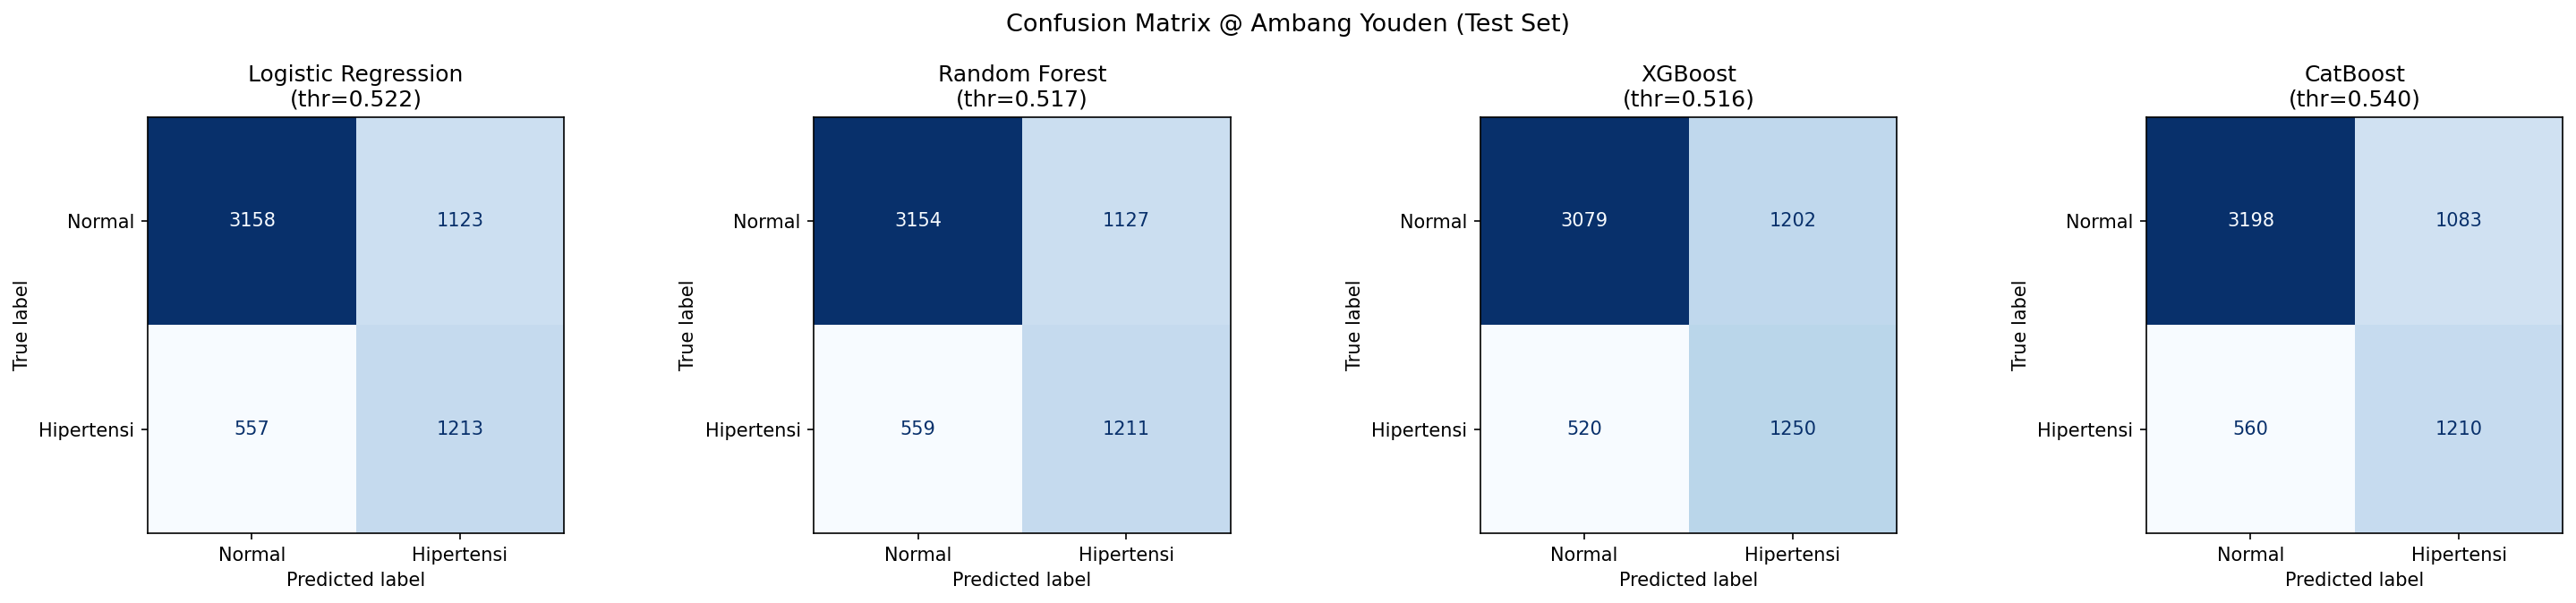
\includegraphics[width=\textwidth]{images/confusion_matrix_youden.png}
\caption{Confusion matrix model setelah tuning pada ambang Youden}
\label{fig:cm}
\end{figure}

Setiap \emph{confusion matrix} memuat empat komponen. \emph{True positive} adalah pasien hipertensi yang diprediksi hipertensi. \emph{True negative} adalah orang normal yang diprediksi normal. \emph{False positive} adalah orang normal yang diprediksi hipertensi. \emph{False negative} adalah pasien hipertensi yang diprediksi normal.

Pada konteks hipertensi, \emph{false negative} adalah komponen yang paling perlu diperhatikan karena mewakili pasien berisiko yang lolos dari deteksi dan berpotensi tidak mendapat penanganan dini. Data uji memuat sekitar 1.770 pasien hipertensi dan sekitar 4.281 orang normal. Untuk XGBoost pada ambang Youden dengan recall 0,7062, jumlah \emph{false negative} berada di kisaran 520 pasien, sedangkan jumlah \emph{true positive} berada di kisaran 1.250 pasien. Angka \emph{false negative} yang masih cukup besar ini menunjukkan bahwa model belum menangkap seluruh pasien berisiko, sehingga hasilnya lebih tepat digunakan sebagai alat bantu skrining awal, bukan sebagai pengganti diagnosis klinis.

% ---------------------------------------------------------------------
\subsubsection{ROC Curve}
\label{subsec:roc-curve}
Gambar~\ref{fig:roc} menampilkan kurva ROC keempat model beserta titik ambang Youden masing-masing.

\begin{figure}[H]
\centering
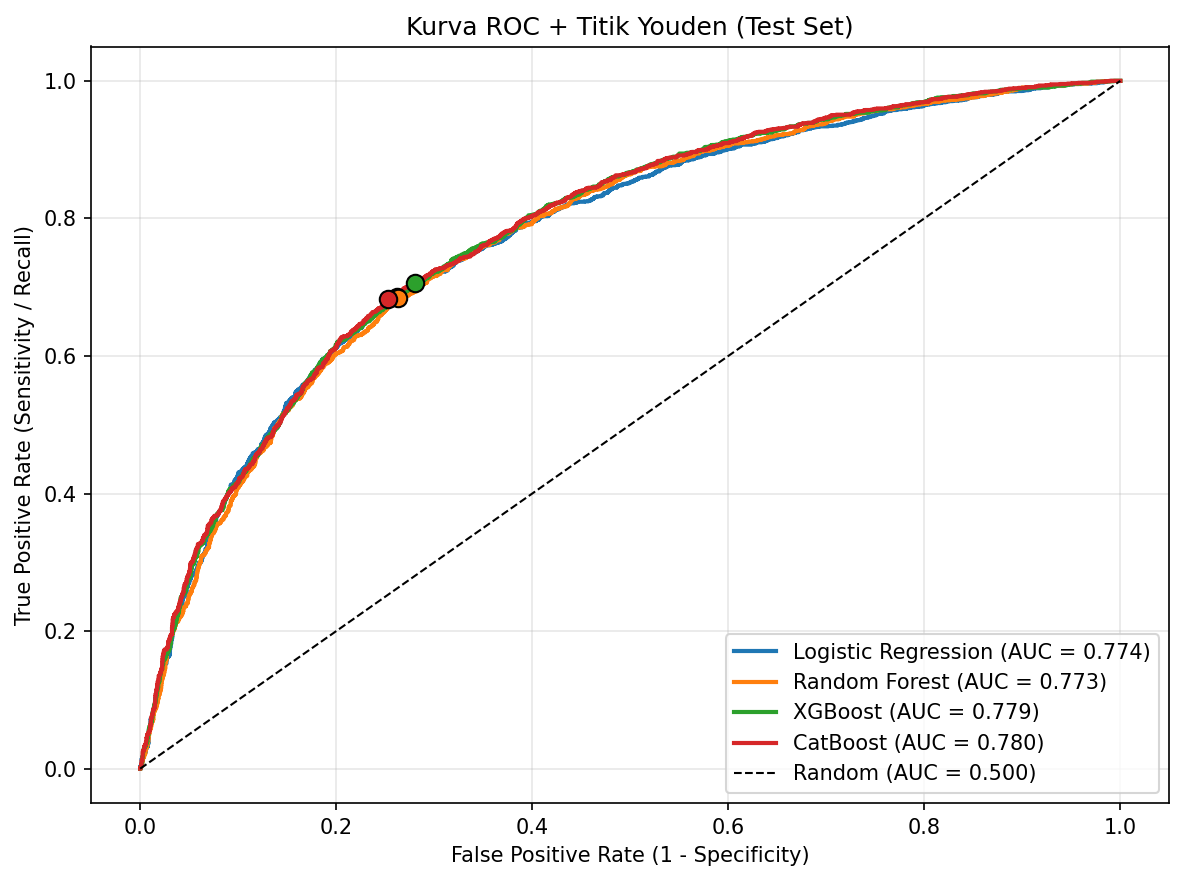
\includegraphics[width=0.85\textwidth]{images/roc_curve_youden.png}
\caption{Kurva ROC dan titik Youden tiap model pada data uji}
\label{fig:roc}
\end{figure}

Kurva ROC menggambarkan hubungan antara \emph{true positive rate} dan \emph{false positive rate} pada seluruh rentang ambang. Semakin dekat kurva ke sudut kiri atas, semakin baik kemampuan model membedakan kelas. Berdasarkan Gambar~\ref{fig:roc}, kurva CatBoost dan XGBoost berada paling dekat dengan sudut kiri atas, sejalan dengan nilai ROC-AUC keduanya yang tertinggi, yaitu 0,7804 untuk CatBoost dan 0,7795 untuk XGBoost. Kurva Logistic Regression dan Random Forest berada sedikit di bawahnya dengan ROC-AUC di kisaran 0,7735. Perbedaan antar model tergolong kecil, yang menunjukkan bahwa keempat model memiliki kemampuan membedakan kelas yang setara pada data ini.

% ---------------------------------------------------------------------
\subsubsection{Pemilihan Model Terbaik}
\label{subsec:pemilihan-model}
Pemilihan model akhir tidak hanya didasarkan pada satu metrik, melainkan pada beberapa pertimbangan sekaligus, yaitu kemampuan membedakan kelas, kemampuan menangkap pasien berisiko, kemudahan penafsiran, dukungan analisis kontribusi fitur, serta kemudahan penerapan pada sistem.

Dari sisi ROC-AUC, CatBoost dan XGBoost hampir setara, dengan selisih hanya 0,0009. Selisih sekecil ini tidak cukup untuk menyatakan salah satu unggul secara meyakinkan. Dari sisi recall pada ambang bawaan 0,5, XGBoost memperoleh nilai tertinggi sebesar 0,7186, yang berarti paling banyak menangkap pasien hipertensi. Karena tujuan utama sistem adalah skrining risiko, kemampuan menangkap pasien berisiko diberi bobot penting.

XGBoost juga memiliki dukungan yang matang untuk analisis kontribusi fitur berbasis SHAP, sehingga hasil prediksi dapat dijelaskan per fitur maupun per pasien. Kemampuan menjelaskan ini penting pada konteks kesehatan agar keputusan model dapat dipahami. Dari sisi penerapan, XGBoost tersedia luas, ringan saat prediksi, dan mudah disimpan lalu dimuat kembali pada sistem, sehingga cocok untuk diintegrasikan pada layanan skrining.

Berdasarkan gabungan pertimbangan tersebut, yaitu kemampuan membedakan kelas yang setara dengan model terbaik, recall tertinggi, dukungan penjelasan berbasis SHAP, serta kemudahan penerapan, XGBoost dipilih sebagai model akhir. Dengan ROC-AUC 0,7795 serta recall 0,7186 pada ambang 0,5 dan 0,7062 pada ambang Youden, XGBoost memenuhi kriteria keberhasilan yang ditetapkan di awal, yaitu ROC-AUC minimal 0,75 dan recall minimal 0,70. Model XGBoost terbaik disimpan bersama nilai ambang Youden dan urutan nama fitur, agar proses prediksi pada sistem memakai konfigurasi yang sama persis dengan hasil eksperimen.


\subsection{Implementasi XAI}
\label{subsec:implementasi-xai}

Setelah XGBoost terpilih sebagai model akhir, dilakukan interpretasi model menggunakan \emph{Explainable AI} berbasis SHAP (\emph{SHapley Additive exPlanations}) untuk menjelaskan dasar setiap prediksi. SHAP mengukur kontribusi tiap fitur terhadap keluaran model berdasarkan teori nilai Shapley, yaitu dengan menimbang dampak rata-rata sebuah fitur ketika diperhitungkan pada berbagai kombinasi fitur lain. Sifatnya aditif, sehingga penjumlahan nilai dasar (\emph{base value}) dengan seluruh kontribusi fitur akan menghasilkan kembali keluaran model untuk satu individu. Dengan demikian, setiap penjelasan dapat dipertanggungjawabkan secara matematis, baik pada tingkat populasi maupun individu.

Penyajian nilai SHAP menggunakan pendekatan gabungan, yaitu analisis global dalam satuan \emph{log-odds} yang merupakan keluaran mentah model, dan analisis lokal dalam satuan probabilitas agar lebih mudah dipahami pengguna. Perlu dicatat bahwa model XGBoost dilatih dengan pembobotan kelas positif untuk menangani ketidakseimbangan data, sehingga rata-rata keluaran probabilistik model berada di sekitar 0,45, lebih tinggi dibandingkan prevalensi hipertensi pada data pemodelan yang sebesar 29,26\%.

\subsubsection{Pemilihan Explainer}

SHAP menyediakan dua explainer yang relevan, yaitu \emph{KernelExplainer} yang bersifat \emph{model-agnostic} namun berbeban komputasi tinggi, dan \emph{TreeExplainer} yang dirancang khusus untuk model berbasis pohon seperti XGBoost sehingga dapat menghitung kontribusi fitur secara eksak dan efisien. Keduanya dibandingkan untuk memastikan pilihan yang tepat, dan hasilnya disajikan pada Tabel~\ref{tab:shap-explainer}. Nilai kontribusi yang dihasilkan kedua metode nyaris identik, dengan rata-rata selisih hanya 0,0014 dan perbedaan kontribusi sebesar 0,44\%. Namun, TreeExplainer jauh lebih cepat, yaitu 0,139 detik dibandingkan 2,438 detik, sehingga TreeExplainer dipilih sebagai metode interpretasi utama.

\begin{table}[htbp]
    \centering
    \caption{Perbandingan KernelExplainer dan TreeExplainer pada 50 Sampel Uji}
    \label{tab:shap-explainer}
    \begin{tabular}{@{}lrr@{}}
        \toprule
        \textbf{Metrik} & \textbf{KernelExplainer} & \textbf{TreeExplainer} \\
        \midrule
        Waktu komputasi (detik) & 2,4382 & 0,1390 \\
        Rata-rata selisih nilai SHAP & \multicolumn{2}{c}{0,0014} \\
        Rata-rata perbedaan kontribusi & \multicolumn{2}{c}{0,44\%} \\
        \bottomrule
    \end{tabular}
\end{table}

\subsubsection{Analisis Global}

Analisis global merangkum kontribusi fitur di seluruh data untuk mengetahui fitur yang paling menentukan estimasi model. Gambar~\ref{fig:shap-bar} menyajikan tingkat kepentingan fitur berdasarkan rata-rata nilai absolut SHAP. Usia merupakan fitur paling dominan, diikuti indeks massa tubuh (IMT) dan jenis kelamin, sedangkan fitur lain seperti kualitas tidur, gangguan tidur, status merokok, kolesterol tinggi, dan diabetes memberikan kontribusi yang jauh lebih kecil. Pola ini mengindikasikan bahwa model bertumpu terutama pada faktor demografis dan komposisi tubuh dalam mengestimasi risiko hipertensi.

\begin{figure}[htbp]
    \centering
    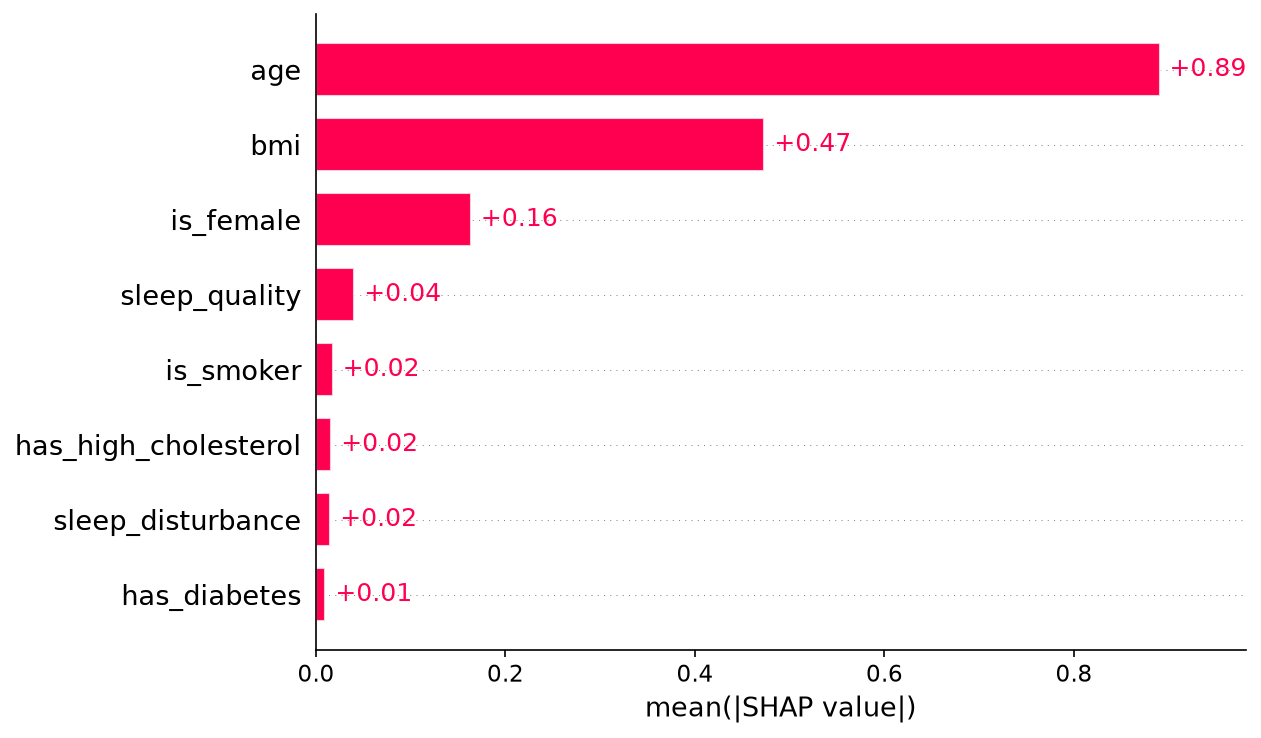
\includegraphics[width=0.7\textwidth]{images/xai/global_bar_mean_abs.png}
    \caption{Tingkat Kepentingan Fitur Berdasarkan Rata-rata Nilai Absolut SHAP}
    \label{fig:shap-bar}
\end{figure}

Gambar~\ref{fig:shap-beeswarm} menampilkan sebaran kontribusi setiap fitur, dengan warna menyatakan nilai fitur (biru untuk rendah, merah untuk tinggi) dan posisi horizontal menyatakan arah serta besar dampaknya. Pada usia dan IMT, nilai tinggi berada di sisi positif sehingga menaikkan estimasi risiko, sedangkan nilai rendah menurunkannya. Pada jenis kelamin, laki-laki cenderung menaikkan estimasi risiko dibandingkan perempuan. Lebar sebaran titik pada setiap baris menggambarkan besarnya variasi pengaruh fitur di antara seluruh sampel.

\begin{figure}[htbp]
    \centering
    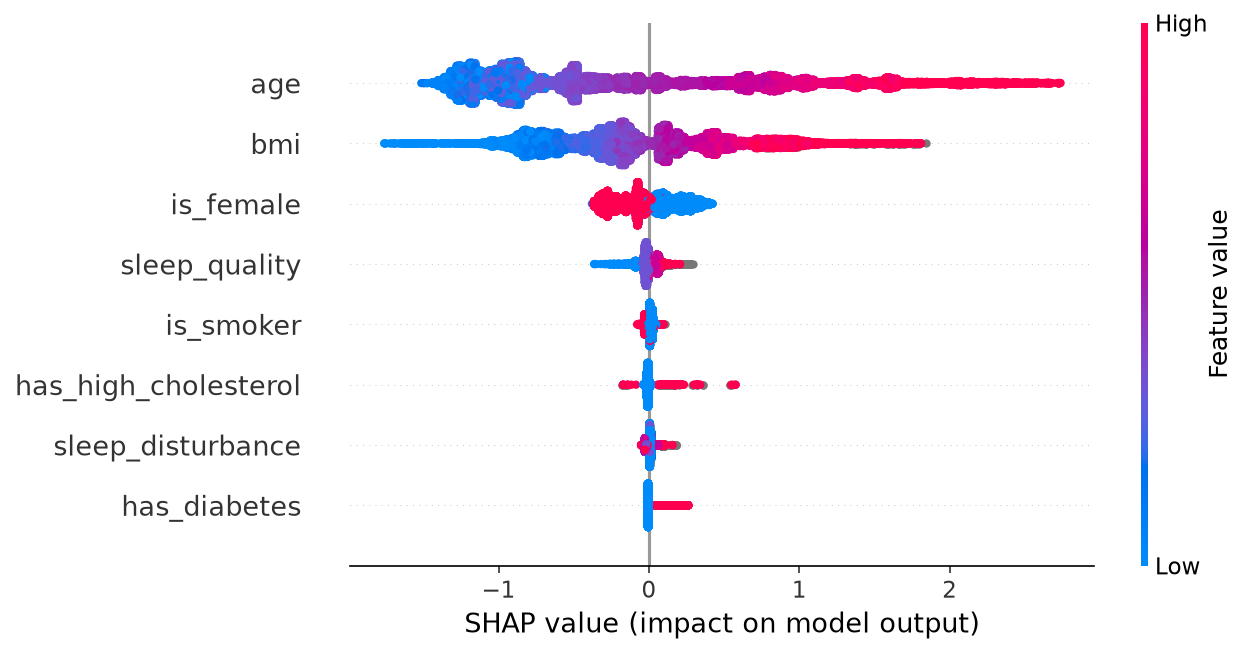
\includegraphics[width=0.8\textwidth]{images/xai/global_beeswarm.png}
    \caption{Sebaran Nilai SHAP Seluruh Fitur (\emph{beeswarm})}
    \label{fig:shap-beeswarm}
\end{figure}

Untuk memahami hubungan tiap fitur secara lebih rinci, distribusi nilai SHAP ditinjau melalui \emph{dependence plot}. Gambar~\ref{fig:shap-age} memperlihatkan kontribusi fitur \textit{age} yang mengikuti pola non-linier, yaitu bernilai negatif pada usia muda di bawah sekitar 30 tahun, meningkat hampir linier mulai sekitar 30 hingga 70 tahun, lalu melandai pada usia lanjut. Pola ini konsisten dengan pengetahuan medis bahwa risiko hipertensi meningkat seiring bertambahnya usia.

\begin{figure}[htbp]
    \centering
    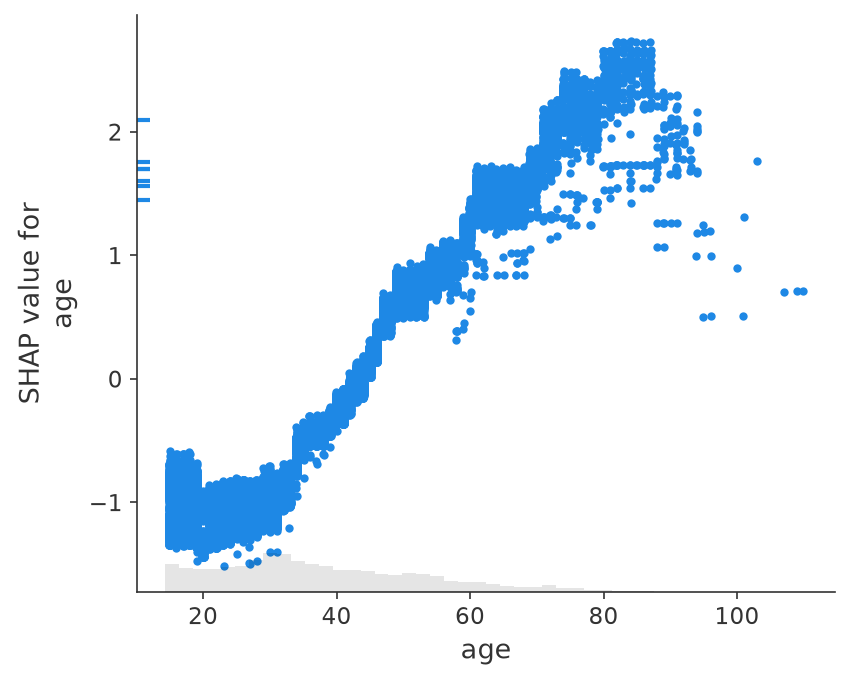
\includegraphics[width=0.6\textwidth]{images/xai/dependence_age.png}
    \caption{Nilai SHAP terhadap Usia}
    \label{fig:shap-age}
\end{figure}

Gambar~\ref{fig:shap-bmi} menampilkan kontribusi fitur \textit{bmi} yang bernilai negatif pada IMT rendah, meningkat tajam pada rentang sekitar 20 hingga 37, lalu cenderung mendatar setelahnya. Hal ini sejalan dengan pemahaman klinis bahwa kelebihan berat badan dan obesitas merupakan faktor risiko hipertensi. Pola tersebut sekaligus menjadikan IMT sebagai fitur berpengaruh terbesar kedua setelah usia.

\begin{figure}[htbp]
    \centering
    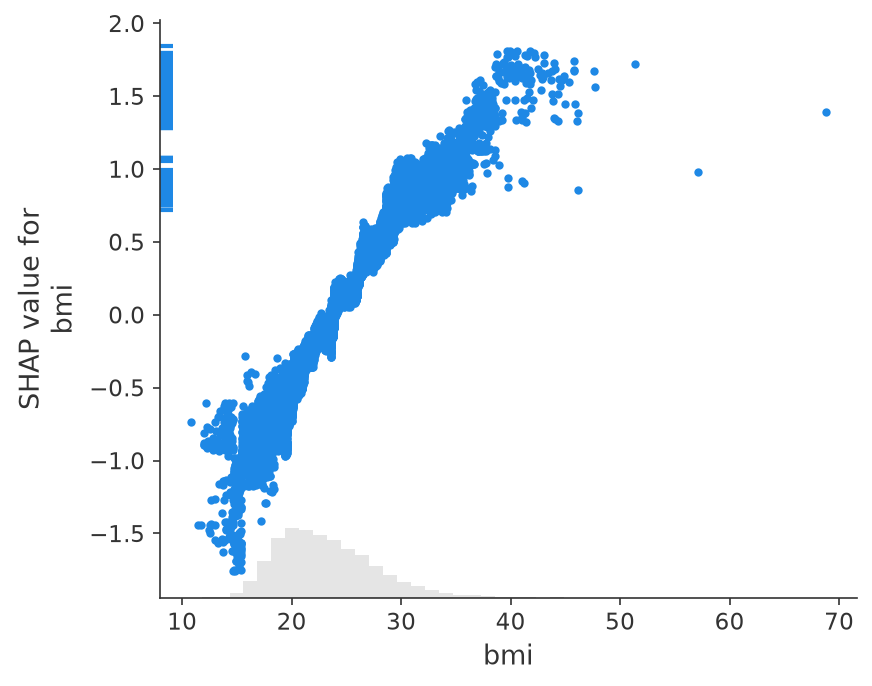
\includegraphics[width=0.6\textwidth]{images/xai/dependence_bmi.png}
    \caption{Nilai SHAP terhadap IMT}
    \label{fig:shap-bmi}
\end{figure}

Gambar~\ref{fig:shap-female} memperlihatkan kontribusi fitur \textit{is\_female}. Individu laki-laki cenderung memiliki nilai SHAP positif, sedangkan perempuan cenderung negatif. Dengan kata lain, model mengaitkan jenis kelamin laki-laki dengan peningkatan estimasi risiko hipertensi. Arah ini selaras dengan temuan epidemiologis yang menunjukkan prevalensi hipertensi yang lebih tinggi pada laki-laki, khususnya pada usia dewasa hingga paruh baya. Sebaran nilai pada masing-masing kategori juga mengindikasikan adanya interaksi dengan fitur lain seperti usia dan IMT.

\begin{figure}[htbp]
    \centering
    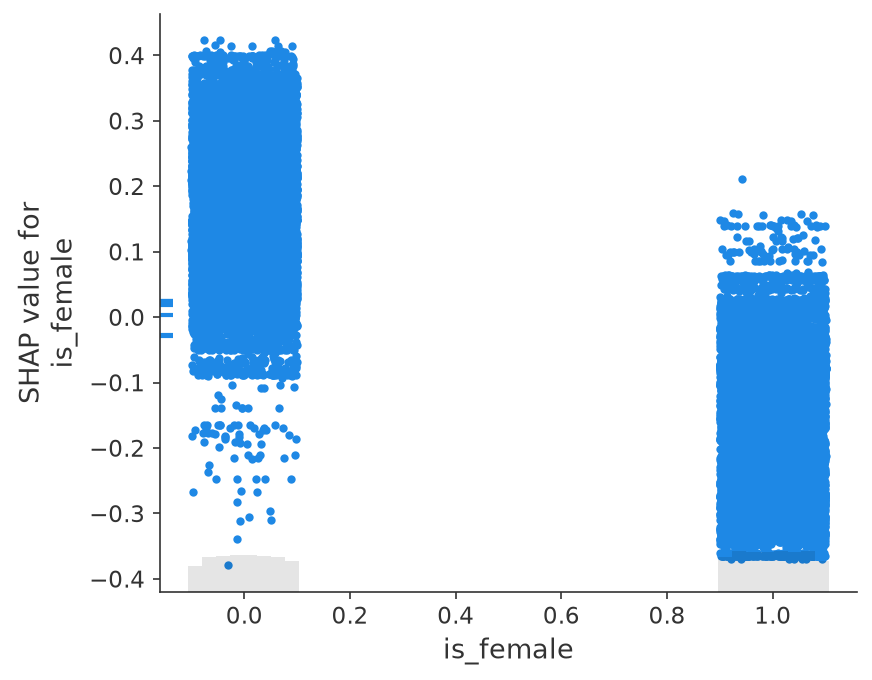
\includegraphics[width=0.6\textwidth]{images/xai/dependence_is_female.png}
    \caption{Nilai SHAP terhadap Jenis Kelamin}
    \label{fig:shap-female}
\end{figure}

Gambar~\ref{fig:shap-disturbance} menampilkan kontribusi fitur \textit{sleep\_disturbance}. Secara umum, semakin tinggi tingkat gangguan tidur, nilai SHAP cenderung semakin positif, sehingga model menangkap kecenderungan bahwa frekuensi gangguan tidur yang lebih tinggi berkaitan dengan estimasi risiko yang lebih besar, sejalan dengan literatur mengenai hubungan antara kualitas istirahat dan tekanan darah. Meskipun demikian, arah global yang positif ini disertai sebaran nilai SHAP yang cukup lebar pada setiap tingkatan, sehingga pada sebagian individu kontribusi fitur ini masih dapat bernilai negatif atau menurunkan estimasi risiko meskipun tren keseluruhannya menaikkan risiko. Variasi pada tingkat individu tersebut timbul karena adanya interaksi dengan fitur lain dan karena besar pengaruh fitur ini tergolong kecil dibandingkan usia dan IMT, sehingga interpretasi lokalnya perlu dilakukan secara hati-hati dan tidak selalu searah dengan tren global.

\begin{figure}[htbp]
    \centering
    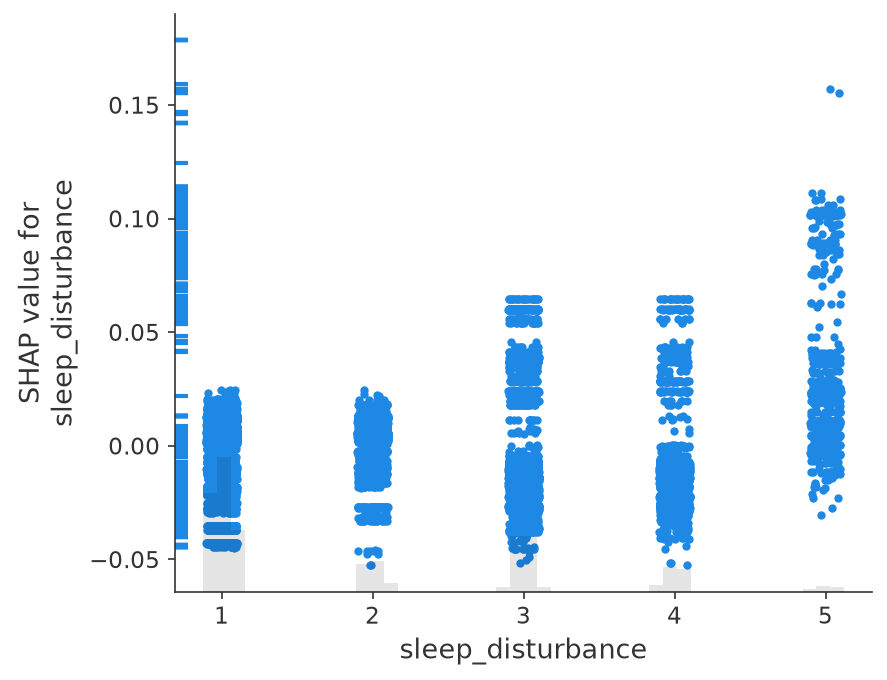
\includegraphics[width=0.6\textwidth]{images/xai/dependence_sleep_disturbance.png}
    \caption{Nilai SHAP terhadap Gangguan Tidur}
    \label{fig:shap-disturbance}
\end{figure}

Gambar~\ref{fig:shap-quality} menampilkan kontribusi fitur \textit{sleep\_quality}. Mengikuti skala IFLS yang dipakai model, yaitu nilai 1 untuk kualitas tidur terbaik hingga 5 untuk terburuk, kualitas tidur yang makin buruk (nilai makin tinggi) memberikan kontribusi SHAP positif yang menaikkan estimasi risiko, sedangkan kualitas tidur yang baik (nilai rendah) menurunkannya. Arah ini konsisten dengan literatur yang menghubungkan kualitas tidur buruk dengan peningkatan risiko hipertensi, meskipun besar pengaruhnya tergolong kecil.

Sebaliknya, satu fitur menunjukkan pola yang berlawanan dengan dugaan umum. Pada Gambar~\ref{fig:shap-smoker}, fitur \textit{is\_smoker} memberikan kontribusi yang sedikit negatif dibandingkan individu yang tidak merokok. Pola ini berpengaruh kecil dan diduga dipengaruhi oleh faktor perancu (\emph{confounding}) pada data survei, sehingga perlu ditinjau lebih lanjut bersama tenaga medis dan tidak dimaknai sebagai hubungan sebab-akibat.

\begin{figure}[htbp]
    \centering
    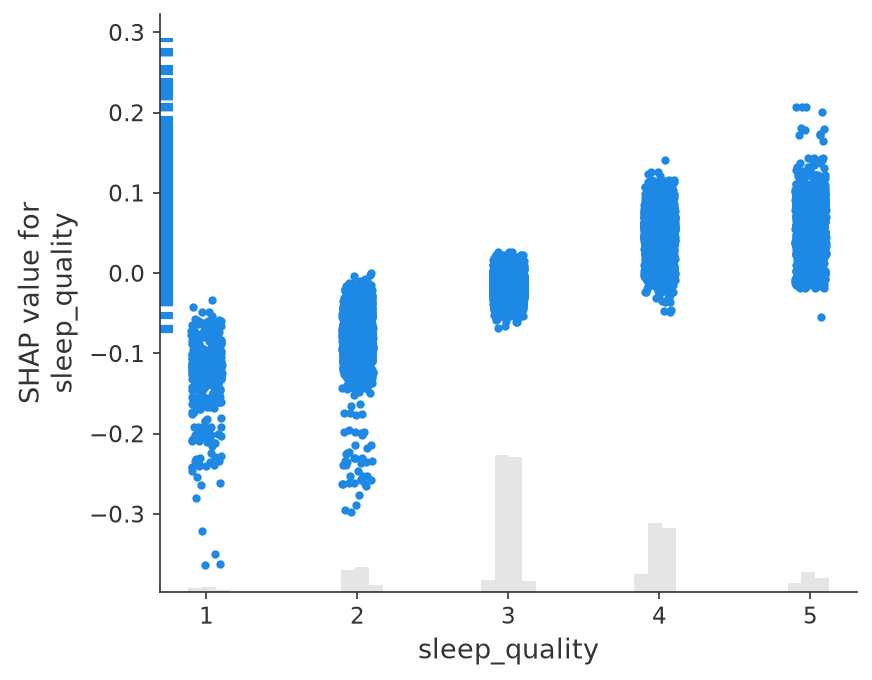
\includegraphics[width=0.6\textwidth]{images/xai/dependence_sleep_quality.png}
    \caption{Nilai SHAP terhadap Kualitas Tidur}
    \label{fig:shap-quality}
\end{figure}

\begin{figure}[htbp]
    \centering
    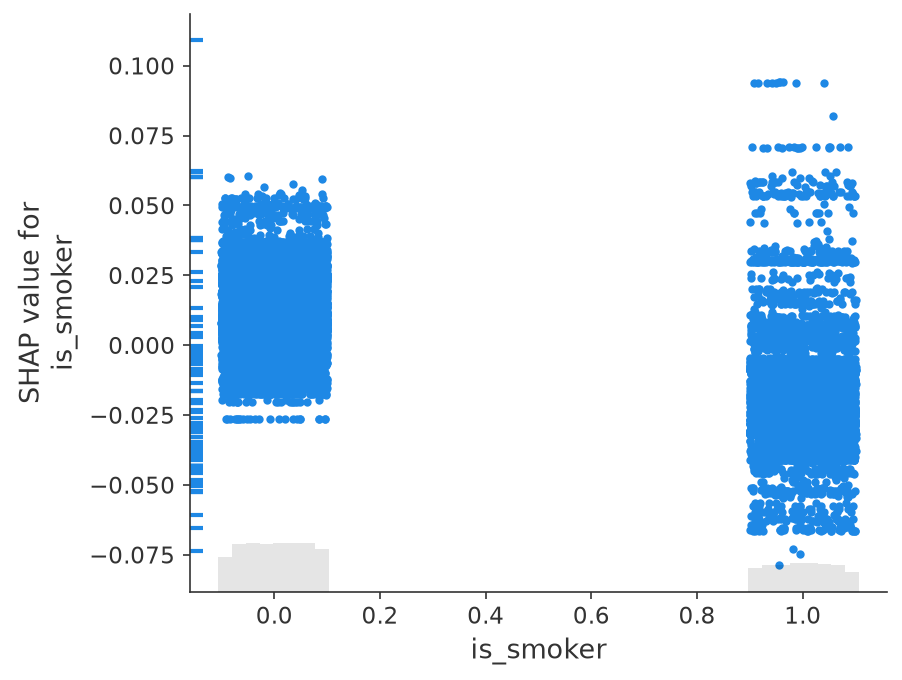
\includegraphics[width=0.6\textwidth]{images/xai/dependence_is_smoker.png}
    \caption{Nilai SHAP terhadap Status Merokok}
    \label{fig:shap-smoker}
\end{figure}

Gambar~\ref{fig:shap-diabetes} dan Gambar~\ref{fig:shap-cholesterol} menampilkan kontribusi fitur \textit{has\_diabetes} dan \textit{has\_high\_cholesterol}. Individu dengan riwayat kedua kondisi tersebut memiliki nilai SHAP positif yang menaikkan estimasi risiko. Arah ini sesuai dengan pemahaman medis mengenai keterkaitan kedua kondisi tersebut dengan tekanan darah. Akan tetapi, sebaran nilainya cukup lebar dan kontribusinya kecil secara keseluruhan. Hal ini disebabkan oleh proporsi data positif yang sangat sedikit untuk kedua fitur, sehingga model kurang memiliki cukup contoh untuk mempelajari polanya secara stabil, dan keterbatasan ini perlu dicatat dalam interpretasi.

\begin{figure}[htbp]
    \centering
    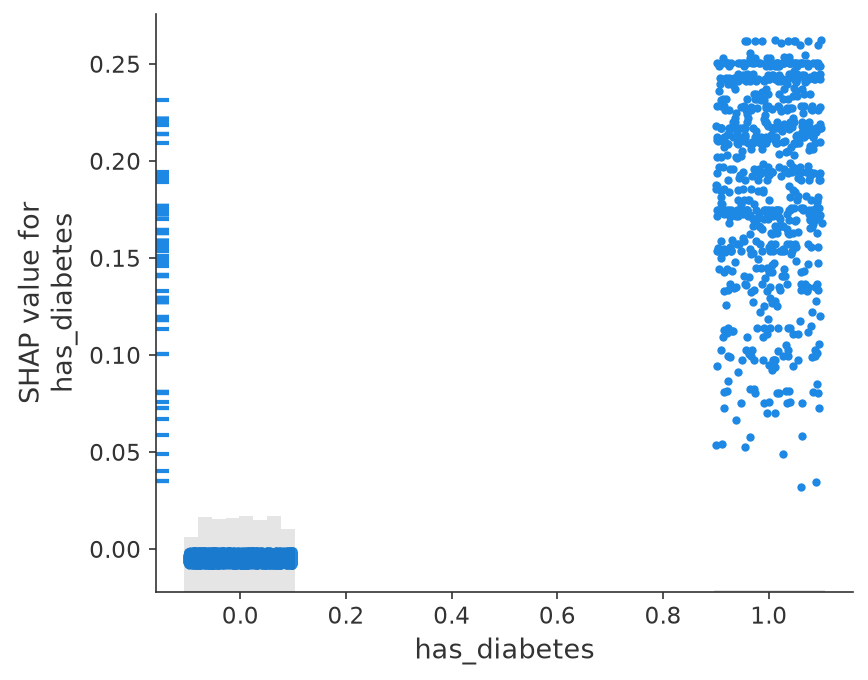
\includegraphics[width=0.6\textwidth]{images/xai/dependence_has_diabetes.png}
    \caption{Nilai SHAP terhadap Riwayat Diabetes}
    \label{fig:shap-diabetes}
\end{figure}

\begin{figure}[htbp]
    \centering
    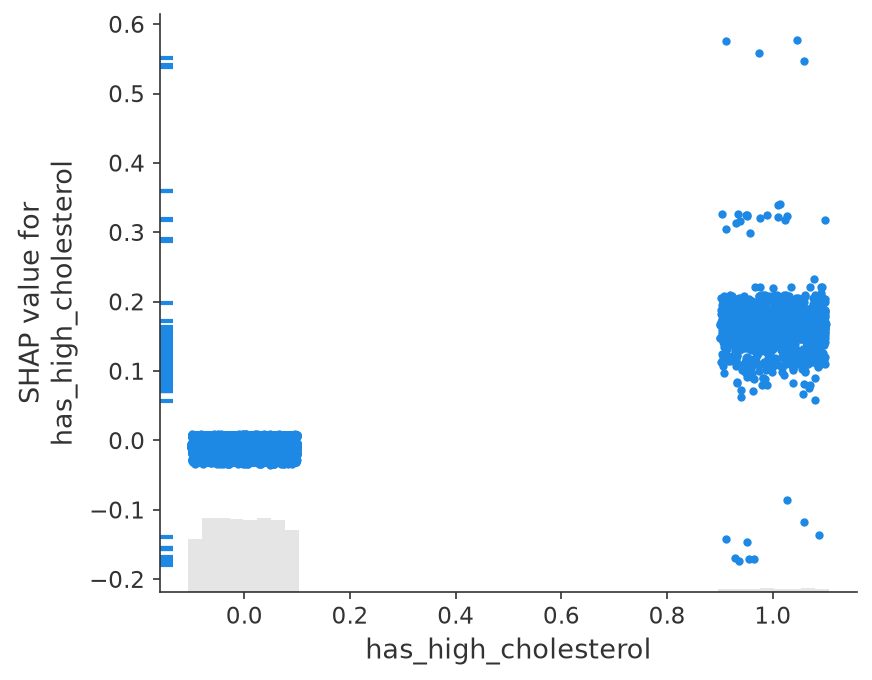
\includegraphics[width=0.6\textwidth]{images/xai/dependence_has_high_cholesterol.png}
    \caption{Nilai SHAP terhadap Riwayat Kolesterol Tinggi}
    \label{fig:shap-cholesterol}
\end{figure}

\subsubsection{Ambang Netral dan Kategori Risiko Terendah}

Selain meninjau arah dan besar kontribusi, nilai SHAP dapat dimanfaatkan untuk memperkirakan ambang nilai yang netral bagi tiap fitur. Untuk fitur kontinu, ambang netral didefinisikan sebagai nilai fitur ketika kontribusi SHAP-nya mendekati nol, yaitu titik saat fitur tidak menaikkan maupun menurunkan estimasi risiko. Untuk fitur biner atau ordinal, ditinjau kategori dengan rata-rata nilai SHAP terendah, yaitu kategori yang paling menurunkan estimasi risiko. Ringkasan hasilnya disajikan pada Tabel~\ref{tab:shap-ambang}.

\begin{table}[htbp]
    \centering
    \caption{Ambang Netral dan Kategori Risiko Terendah Tiap Fitur}
    \label{tab:shap-ambang}
    \begin{tabularx}{\textwidth}{@{}l l p{3.2cm} X@{}}
        \toprule
        \textbf{Fitur} & \textbf{Tipe} & \textbf{Ambang / kategori terendah} & \textbf{Keterangan} \\
        \midrule
        Usia & Kontinu & $\approx$ 43 tahun (40--45) & Arah positif; nilai di bawah ambang menurunkan risiko \\
        IMT & Kontinu & $\approx$ 24 (22--25) & Arah positif; IMT normal menurunkan risiko \\
        Jenis kelamin & Biner & Perempuan & Laki-laki cenderung menaikkan risiko \\
        Diabetes & Biner & Tidak diabetes & Sesuai pemahaman medis \\
        Kolesterol tinggi & Biner & Tidak kolesterol tinggi & Sesuai pemahaman medis \\
        Gangguan tidur & Ordinal & Tingkat terendah & Gangguan lebih tinggi menaikkan risiko \\
        Status merokok & Biner & Tidak ditafsirkan & Pola berlawanan dengan medis; perlu evaluasi \\
        Kualitas tidur & Ordinal & Kualitas terbaik & Kualitas tidur lebih buruk menaikkan risiko \\
        \bottomrule
    \end{tabularx}
\end{table}

Pada fitur kontinu, usia memiliki ambang netral sekitar 43 tahun dan IMT sekitar 24, keduanya dengan arah positif, sehingga nilai di bawah ambang cenderung menurunkan estimasi risiko dan di atasnya menaikkannya. Ambang IMT sekitar 24 menarik karena berdekatan dengan batas atas kategori IMT normal menurut standar kesehatan, sehingga model secara implisit menempatkan rentang IMT normal sebagai kondisi yang relatif netral. Pada fitur biner dan ordinal, kategori dengan risiko terendah umumnya sejalan dengan pemahaman medis, yaitu tidak memiliki diabetes maupun kolesterol tinggi, serta tingkat gangguan tidur yang paling rendah dan kualitas tidur yang paling baik. Untuk jenis kelamin, kategori perempuan menunjukkan kontribusi yang lebih menurunkan risiko, meskipun jenis kelamin merupakan karakteristik bawaan dan bukan pilihan yang dapat diubah.

Perlu ditekankan bahwa pendekatan ini tidak dapat diterapkan pada seluruh fitur secara langsung. Pada status merokok, kategori dengan nilai SHAP terendah justru bertentangan dengan pengetahuan medis, sehingga tidak layak dimaknai sebagai kondisi ideal. Hal ini sejalan dengan temuan sebelumnya bahwa fitur tersebut memiliki pola yang berlawanan dengan dugaan umum dan diduga dipengaruhi oleh faktor perancu pada data. Dengan demikian, penentuan nilai ideal berbasis SHAP harus selalu divalidasi terhadap pengetahuan domain sebelum digunakan sebagai dasar rekomendasi.

\subsubsection{Analisis Lokal}

Selain analisis global, SHAP juga dapat menjelaskan estimasi untuk satu individu secara terpisah. Pada analisis lokal yang disajikan dalam satuan probabilitas, estimasi dimulai dari nilai dasar sekitar 0,45 atau 45\%, yaitu rata-rata keluaran model atas data. Nilai dasar yang relatif tinggi ini merupakan akibat penerapan pembobotan kelas saat pelatihan, dan bukan prevalensi hipertensi pada data pemodelan yang sebesar 29,26\%. Dari titik awal tersebut, setiap fitur menambah atau mengurangi nilai estimasi sesuai kontribusinya hingga diperoleh keluaran akhir model untuk individu bersangkutan.

Gambar~\ref{fig:shap-lokal} menunjukkan contoh analisis lokal untuk seorang individu berusia 59 tahun, berjenis kelamin laki-laki, dengan IMT 24,1, kualitas tidur baik, serta tanpa riwayat diabetes maupun kolesterol tinggi. Estimasi akhir model untuk individu ini adalah sekitar 0,76 atau 76,2\%, sehingga tergolong berisiko tinggi. Kontribusi positif terbesar berasal dari usia (sekitar 0,27), diikuti oleh jenis kelamin laki-laki dan IMT yang besarnya sebanding (sekitar 0,04 dan 0,03), sementara kualitas tidur dan status merokok memberikan kontribusi negatif yang kecil. Dengan demikian, peningkatan estimasi risiko pada individu ini didorong terutama oleh faktor usia.

\begin{figure}[htbp]
    \centering
    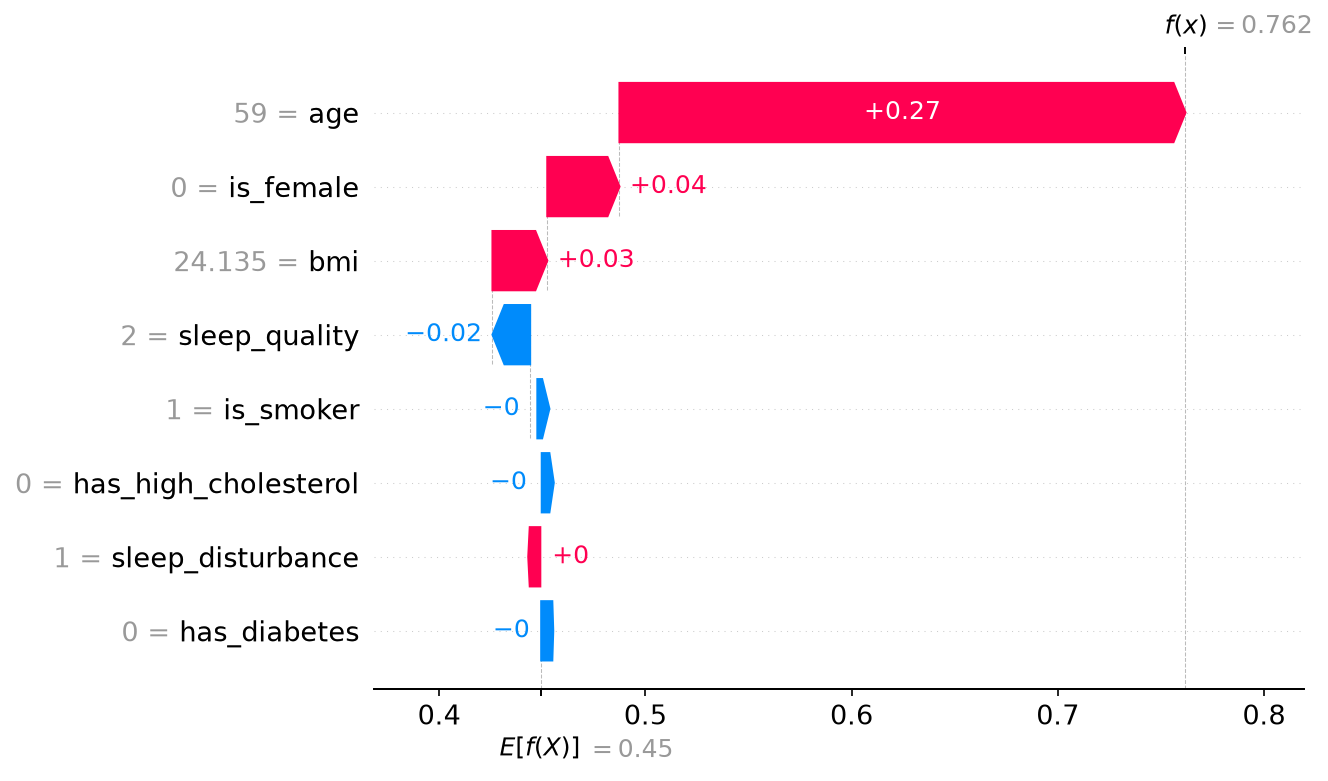
\includegraphics[width=0.8\textwidth]{images/xai/local_waterfall_prob_idx0.png}
    \caption{Contoh Analisis Lokal SHAP untuk Satu Individu (Satuan Probabilitas)}
    \label{fig:shap-lokal}
\end{figure}

\subsubsection{Evaluasi dan Keterbatasan}

Hasil interpretasi SHAP dievaluasi untuk memastikan kelayakannya secara klinis. Sebagian besar pola yang dihasilkan model selaras dengan pemahaman medis, yaitu usia, IMT, jenis kelamin laki-laki, kualitas tidur, gangguan tidur, diabetes, dan kolesterol tinggi yang berkontribusi menaikkan estimasi risiko hipertensi. Sebaliknya, terdapat satu pola yang berlawanan dengan dugaan umum, yaitu pada status merokok, yang berpengaruh kecil dan diduga dipengaruhi oleh faktor perancu pada data survei. Selain itu, fitur diabetes dan kolesterol tinggi memiliki keterbatasan berupa jumlah data positif yang sangat sedikit sehingga interpretasinya kurang stabil, sehingga pola yang tidak intuitif maupun fitur dengan data terbatas tersebut direkomendasikan untuk dikonfirmasi lebih lanjut melalui evaluasi oleh tenaga medis atau \emph{domain expert} sebelum digunakan dalam pengambilan keputusan.


% Catatan bibliografi: perintah \autocite di bawah memakai kunci
%   zeng2024shapllm -> Zeng & Zhu (2024), interpretasi nilai SHAP dengan LLM
% Sesuaikan kunci ini dengan berkas .bib Anda, atau hapus \autocite bila belum ada.
% ======================================================================

\subsection{Implementasi Narasi Medis berbasis Kaidah Deterministik dan LLM}
\label{subsec:implementasi-narasi}

Interpretasi SHAP pada subbab~\ref{subsec:implementasi-xai} menghasilkan kontribusi tiap fitur, baik secara global maupun untuk satu individu, dalam bentuk nilai numerik. Bentuk numerik ini tepat secara matematis namun sulit dipahami oleh pengguna awam. Oleh karena itu, dibangun sebuah lapisan narasi yang menerjemahkan nilai SHAP menjadi penjelasan berbahasa Indonesia yang mudah dicerna pasien, mengikuti gagasan pemanfaatan LLM untuk meningkatkan keterbacaan nilai SHAP \autocite{zeng2024shapllm}, mencakup faktor risiko yang paling berpengaruh beserta arahnya, serta saran perbaikan gaya hidup. Karena keluaran ini menyentuh ranah kesehatan, prioritas utama perancangannya adalah menekan halusinasi dan misinformasi, sehingga penggunaan \emph{Large Language Model} (LLM) dibatasi secara ketat.

Kebutuhan pembatasan ini diperkuat oleh temuan pada subbab~\ref{subsec:implementasi-xai}. Sebagaimana dirangkum pada Tabel~\ref{tab:shap-ambang}, satu fitur, yaitu status merokok, memiliki arah kontribusi yang berlawanan dengan pengetahuan medis dan ditandai ``tidak ditafsirkan''. Apabila arah SHAP fitur tersebut diterjemahkan mentah-mentah menjadi kalimat untuk pasien, sistem berpotensi menyatakan bahwa merokok menurunkan risiko hipertensi, yang merupakan misinformasi berbahaya. Lapisan narasi ini dirancang untuk mengoperasionalkan peringatan tersebut secara otomatis.

\subsubsection{Arsitektur Narasi}

Narasi dibangun melalui dua lapisan dengan pembagian tugas yang tegas, sebagaimana dirangkum pada Tabel~\ref{tab:arsitektur-narasi}. Prinsip utamanya adalah seluruh \emph{angka} dan \emph{arah} ditentukan secara deterministik oleh kode, sedangkan LLM hanya bertugas merangkai kalimat saran. Dengan demikian, LLM tidak pernah menghitung persentase, menentukan arah pengaruh, maupun menciptakan anjuran medis baru, sehingga sumber kesalahan faktual dari model generatif dapat dihilangkan pada bagian yang paling kritis.

\begin{table}[htbp]
    \centering
    \caption{Pembagian Tugas Dua Lapisan Penyusun Narasi}
    \label{tab:arsitektur-narasi}
    \begin{tabularx}{\textwidth}{@{}l X l@{}}
        \toprule
        \textbf{Lapisan} & \textbf{Peran} & \textbf{Sifat} \\
        \midrule
        Deterministik & Menentukan arah, besaran, barometer, pemilihan teks fakta, dan penyusunan materi saran dari nilai SHAP serta kondisi klinis & Berbasis aturan \\
        LLM           & Merangkai ulang materi saran menjadi bahasa yang fleksibel dan empatik & Generatif terkendali \\
        \bottomrule
    \end{tabularx}
\end{table}

Setiap prediksi menghasilkan tiga komponen keluaran, yaitu ringkasan tingkat risiko, interpretasi tiga faktor teratas (masing-masing berupa penjelasan objektif dan alasan berbasis fakta), serta satu paragraf saran gaya hidup. Keseluruhan alur penyusunan narasi tersebut diringkas sebagai pseudocode pada Algoritma~\ref{alg:narasi}.

\begin{algorithm}[htbp]
\caption{Penyusunan Narasi Penjelasan Berbasis Kaidah Deterministik dan LLM}
\label{alg:narasi}
\begin{algorithmic}[1]
\Require Nilai SHAP individu $\{\phi_i\}$, data klinis pasien, probabilitas risiko $p$
\Ensure Narasi penjelasan berbahasa Indonesia
\State Tetapkan tingkat risiko dari $p$ memakai ambang Youden (tinggi atau rendah)
\ForAll{fitur $i$}
    \State $\mathit{arah}_i \gets \operatorname{tanda}(\phi_i)$ \Comment{positif menaikkan, negatif menurunkan risiko}
    \State $\mathit{kontribusi}_i \gets |\phi_i| / \sum_{j} |\phi_j| \times 100\%$
    \State $\mathit{kategori}_i \gets$ kategorikan besaran $\mathit{kontribusi}_i$
\EndFor
\State Pilih tiga fitur dengan kontribusi terbesar
\ForAll{fitur terpilih $i$}
    \If{$i$ tergolong Tingkat C (mis. status merokok)}
        \State Tolak arah yang keliru; tampilkan fakta medis yang benar \Comment{override}
    \ElsIf{$\mathit{kontribusi}_i < 3\%$}
        \State Sampaikan fakta secara \emph{hedged} tanpa klaim sebab-akibat
    \Else
        \State Susun teks fakta penuh sesuai arah SHAP
    \EndIf
\EndFor
\State Bentuk materi saran deterministik dari faktor klinis yang dapat diubah
\State $\mathit{materi} \gets$ ringkasan risiko $+$ interpretasi tiga faktor $+$ saran
\If{layanan LLM tersedia}
    \State $\mathit{narasi} \gets \operatorname{LLM.haluskan}(\mathit{materi})$ \Comment{guardrail: angka/arah/klaim tidak boleh diubah}
\Else
    \State $\mathit{narasi} \gets \mathit{materi}$ \Comment{fallback deterministik}
\EndIf
\State \Return $\mathit{narasi}$
\end{algorithmic}
\end{algorithm}

\subsubsection{Lapisan Deterministik: Arah, Besaran, dan Barometer}

Arah pengaruh setiap fitur ditentukan langsung dari \emph{tanda} nilai SHAP individu, bukan dari korelasi fitur maupun asumsi. Nilai SHAP positif dimaknai menaikkan estimasi risiko dan nilai negatif menurunkannya. Pilihan ini penting karena pada tahap awal ditemukan bahwa penanda arah berbasis korelasi dapat terbalik terhadap keluaran model sebenarnya, sehingga tanda SHAP per individu dipakai sebagai satu-satunya sumber arah.

Besaran pengaruh dinyatakan sebagai persentase kontribusi lokal, yaitu nilai absolut SHAP sebuah fitur dibagi jumlah nilai absolut SHAP seluruh fitur pada individu tersebut, sebagaimana Persamaan~\eqref{eq:share-lokal}. Perhitungan dilakukan pada satuan \emph{log-odds} yang merupakan ruang aditif SHAP, agar konsisten dengan analisis global.

\begin{equation}
\label{eq:share-lokal}
\text{kontribusi}_i = \frac{|\phi_i|}{\sum_{j=1}^{n} |\phi_j|} \times 100\%
\end{equation}

\noindent dengan $\phi_i$ menyatakan nilai SHAP fitur ke-$i$ dan $n$ jumlah fitur. Persentase ini kemudian dikategorikan menjadi lima tingkat sebagaimana Tabel~\ref{tab:kategori-magnitudo}. Ambang tersebut sekaligus berfungsi sebagai pengaman: faktor dengan kontribusi di bawah 3\% dinyatakan dapat diabaikan, sehingga sistem tidak membuat klaim tegas atas faktor yang pengaruhnya tidak berarti.

\begin{table}[htbp]
    \centering
    \caption{Kategori Besaran Pengaruh Berdasarkan Kontribusi Lokal}
    \label{tab:kategori-magnitudo}
    \begin{tabular}{@{}ll@{}}
        \toprule
        \textbf{Kategori} & \textbf{Rentang Kontribusi} \\
        \midrule
        Dominan       & $\geq$ 50\% \\
        Kuat          & 25\%--49,9\% \\
        Moderat       & 10\%--24,9\% \\
        Kecil         & 3\%--9,9\% \\
        Sangat kecil  & $<$ 3\% \\
        \bottomrule
    \end{tabular}
\end{table}

Agar penjelasan objektif terasa membumi, nilai indeks massa tubuh dibandingkan terhadap sebuah barometer, yaitu klasifikasi baku WHO: kurang dari 18,5 sebagai kurus, 18,5 sampai 24,9 sebagai normal, 25 sampai 29,9 sebagai berlebih, dan 30 ke atas sebagai obesitas. Klasifikasi WHO ini selaras dengan ambang netral IMT model yang berada di sekitar 24, yaitu batas atas kategori normal, sebagaimana dibahas pada Tabel~\ref{tab:shap-ambang}. Untuk usia, nilai ditampilkan apa adanya tanpa label tahap kehidupan, mengingat tidak terdapat satu standar klasifikasi usia baku yang konsisten sehingga penambahan label berpotensi menyesatkan; arah dan besaran pengaruh usia tetap ditentukan dari nilai SHAP-nya.

\subsubsection{Klasifikasi Keandalan Fitur}

Tidak semua fitur layak diberi penjelasan berbasis fakta yang tegas. Berdasarkan kesesuaian arah model dengan bukti medis pada subbab~\ref{subsec:implementasi-xai}, kedelapan fitur dikelompokkan ke dalam tiga tingkat keandalan sebagaimana Tabel~\ref{tab:tier-fitur}. Tingkat A memuat fitur yang arahnya searah dan konsisten dengan bukti medis sehingga memperoleh penjelasan fakta penuh sesuai tanda SHAP. Tingkat B memuat fitur yang pengaruhnya kecil atau arahnya spesifik pada model sehingga penjelasannya disampaikan secara berhati-hati tanpa klaim sebab-akibat. Tingkat C memuat status merokok, satu-satunya fitur yang arah modelnya bertentangan dengan bukti medis.

\begin{table}[htbp]
    \centering
    \caption{Tingkat Keandalan Fitur dan Penanganan Teks Fakta}
    \label{tab:tier-fitur}
    \begin{tabularx}{\textwidth}{@{}c l X@{}}
        \toprule
        \textbf{Tingkat} & \textbf{Fitur} & \textbf{Penanganan teks fakta} \\
        \midrule
        A & Usia, IMT, diabetes, kolesterol tinggi & Fakta penuh, arah mengikuti tanda SHAP \\
        B & Jenis kelamin, kualitas tidur, gangguan tidur & Fakta di-\emph{hedge}; tunduk pada pengaman 3\% \\
        C & Status merokok & Di-\emph{override}: fakta medis yang benar selalu ditampilkan, arah ``protektif'' yang keliru ditolak \\
        \bottomrule
    \end{tabularx}
\end{table}

Penanganan khusus tingkat C bekerja sebagai berikut. Teks objektif untuk status merokok tidak pernah menyatakan arah ``menurunkan risiko'', melainkan hanya menyebut besaran pengaruhnya yang pada praktiknya selalu tergolong sangat kecil. Sementara itu, teks faktanya selalu menyatakan kebenaran medis, yaitu bahwa kebiasaan merokok cenderung meningkatkan risiko hipertensi. Dengan mekanisme ini, artefak model tidak diteruskan menjadi misinformasi, namun informasi yang benar tetap sampai kepada pasien.

\subsubsection{Pembuatan Saran Gaya Hidup}

Saran gaya hidup disusun secara deterministik, bukan dibangkitkan bebas oleh LLM, agar seluruh anjuran dapat dipertanggungjawabkan. Setiap faktor risiko yang dapat diubah memiliki satu potongan anjuran baku yang disusun mengacu pada pengetahuan medis umum dan pedoman hipertensi. Potongan-potongan inilah yang dirangkai menjadi materi saran, sehingga isi anjuran tidak pernah bergantung pada pengetahuan bebas model generatif.

Perbedaan mendasar dari rancangan awal terletak pada pemicu saran. Saran tidak dipicu oleh tanda SHAP, melainkan oleh kondisi klinis nyata pasien, dan hanya menyasar faktor yang dapat diubah. Faktor usia dan jenis kelamin dikecualikan karena tidak dapat dimodifikasi. Sebuah faktor memicu saran apabila indeks massa tubuh mencapai 25 atau lebih, pasien berstatus perokok, memiliki riwayat diabetes atau kolesterol tinggi, atau memiliki gangguan tidur tingkat tinggi maupun kualitas tidur yang rendah. Pemisahan ini memberi manfaat ganda: saran berhenti merokok tetap muncul untuk pasien perokok meskipun SHAP model menandainya ``protektif'', sedangkan pasien dengan IMT normal tidak akan menerima saran penurunan berat badan yang tidak relevan.

Faktor pemicu yang terpilih kemudian disusun menjadi materi saran deterministik yang selalu diawali kalimat ``Berdasarkan faktor tersebut, disarankan pasien untuk\ldots'' dan diakhiri anjuran berkonsultasi dengan tenaga kesehatan. Materi inilah yang diserahkan kepada LLM. Model \textit{llama-3.1-8b-instant} yang diakses melalui layanan Groq hanya diminta menuliskan ulang materi tersebut agar lebih fleksibel, dengan larangan menambah atau mengubah anjuran maupun angka, larangan menyuruh mengubah faktor yang tidak dapat diubah, serta aturan akurasi medis, misalnya kata natrium hanya boleh dirangkai dengan ``membatasi'' atau ``mengurangi''. Apabila layanan LLM tidak tersedia, sistem secara otomatis memakai materi saran deterministik apa adanya sehingga keluaran tetap valid.

\subsubsection{Contoh Keluaran}

Untuk menggambarkan hasil akhir, digunakan kembali individu yang sama dengan contoh analisis lokal pada Gambar~\ref{fig:shap-lokal}, yaitu seorang laki-laki berusia 59 tahun dengan IMT 24,1, berstatus perokok, kualitas tidur baik, serta tanpa riwayat diabetes maupun kolesterol tinggi, dengan estimasi risiko 76,2\%. Narasi yang dihasilkan sistem ditampilkan pada kutipan berikut.

\begin{quote}
\small\itshape
Hasil analisis menunjukkan risiko hipertensi Anda sebesar 76,2\%, yang termasuk kategori tinggi.

Usia Anda yakni 59 tahun, memiliki pengaruh dominan dalam meningkatkan risiko ini, dengan kontribusi 72,7\% dari keseluruhan faktor. Bertambahnya usia meningkatkan risiko hipertensi karena elastisitas dinding arteri menurun dan kekakuan pembuluh darah meningkat seiring waktu.

Indeks massa tubuh (IMT) Anda sebesar 24,1 yang tergolong normal, memiliki pengaruh moderat dalam meningkatkan risiko ini, dengan kontribusi 11,3\% dari keseluruhan faktor. Indeks massa tubuh yang lebih tinggi meningkatkan risiko hipertensi karena menambah beban kerja jantung dan resistensi pembuluh darah.

Kualitas tidur Anda tergolong baik (skor 2 dari 5) dan memiliki pengaruh kecil dalam menurunkan risiko ini, dengan kontribusi 6,6\% dari keseluruhan faktor. Kualitas tidur yang baik berkaitan dengan risiko hipertensi yang lebih rendah, dan karena pengaruhnya tergolong kecil, keterkaitan ini tidak dijadikan klaim sebab-akibat.

Berdasarkan faktor tersebut, disarankan pasien untuk berhenti merokok karena memberi manfaat langsung bagi kesehatan pembuluh darah dan tekanan darah, dan memperbaiki kualitas tidur dengan jadwal tidur yang teratur serta membatasi kafein dan paparan layar sebelum tidur, serta berkonsultasi dengan tenaga kesehatan untuk pemeriksaan dan penanganan lebih lanjut.
\end{quote}

Contoh ini memperlihatkan dua mekanisme pengaman bekerja sekaligus. Pertama, kualitas tidur muncul sebagai faktor ketiga dengan arah menurunkan risiko yang kini konsisten dengan literatur karena kualitas tidur pasien tergolong baik; karena pengaruhnya kecil, teks faktanya tetap di-\emph{hedge} sehingga tidak menjadi klaim sebab-akibat. Kedua, status merokok tidak tampil pada tiga faktor teratas karena kontribusi SHAP-nya sangat kecil dan berarah keliru, tetapi saran berhenti merokok tetap muncul karena dipicu oleh kondisi klinis pasien yang memang seorang perokok. Dengan demikian, keterbatasan model yang diidentifikasi pada subbab~\ref{subsec:implementasi-xai} tidak berubah menjadi misinformasi pada keluaran akhir.

\subsubsection{Evaluasi dan Keterbatasan}

Keandalan faktual narasi bertumpu pada pemisahan tugas: seluruh angka, arah, kategori, dan pemilihan fakta bersifat deterministik dan dapat ditelusuri kembali ke nilai SHAP, sementara peran generatif LLM dibatasi pada penghalusan bahasa saran yang isinya telah ditetapkan secara deterministik. Rancangan ini menekan ruang munculnya halusinasi pada bagian yang paling berisiko.

Meskipun demikian, terdapat sejumlah keterbatasan. Cakupan saran bergantung pada kelengkapan potongan anjuran baku yang disusun, sehingga faktor risiko di luar daftar tersebut belum tertangani. Penggunaan LLM berukuran relatif kecil juga menuntut instruksi yang ketat agar keluaran tetap patuh, dan variasi antar pemanggilan tetap mungkin terjadi. Selain itu, template fakta dan saran medis disusun berdasarkan pengetahuan umum dan pedoman, sehingga tetap memerlukan penelaahan oleh tenaga medis sebelum digunakan pada konteks pelayanan sebenarnya. Sejalan dengan simpulan pada subbab sebelumnya, seluruh keluaran narasi diposisikan sebagai alat bantu edukasi dan skrining awal, bukan pengganti diagnosis maupun nasihat klinis.

\section{Hasil Implementasi Purwarupa}
\label{sec:hasil-prototype}
Bagian ini memaparkan hasil implementasi purwarupa sistem berbasis web yang mengintegrasikan ketiga modul, yaitu model klasifikasi XGBoost, interpretasi SHAP, dan modul narasi berbasis LLM, ke dalam satu alur kerja \emph{end-to-end}. Purwarupa ini berfungsi sebagai bukti konsep (\emph{proof of concept}) yang mendemonstrasikan bahwa ketiga komponen dapat bekerja secara terpadu, mulai dari masukan data faktor risiko non-invasif hingga keluaran berupa status risiko, grafik faktor penyebab, dan narasi penjelasan.

Purwarupa diwujudkan dengan arsitektur berbasis layanan (\emph{service-based}) yang memisahkan antarmuka pengguna (\emph{frontend}) dari mesin analisis (\emph{backend}). Kedua sisi berkomunikasi melalui antarmuka REST berbasis JSON, sehingga seluruh logika prediksi terpusat di backend sementara frontend berfokus pada pengumpulan masukan dan penyajian hasil.

\subsection{Lingkungan dan Teknologi Implementasi}
Antarmuka pengguna dibangun menggunakan kerangka kerja Next.js 14 berbasis React 18 dengan bahasa TypeScript dan penataan gaya Tailwind CSS. Komunikasi ke backend memanfaatkan \textit{fetch} bawaan peramban dalam format JSON, sedangkan visualisasi kontribusi fitur dirender secara mandiri tanpa pustaka grafik pihak ketiga agar tampilan tetap ringan dan terkendali.

Backend dikembangkan dengan kerangka kerja FastAPI (Python) dan mengekspos satu titik akhir utama, yaitu \textit{POST /api/v1/analyze}, yang menerima delapan fitur non-invasif serta mengembalikan hasil prediksi, atribusi SHAP, dan narasi dalam satu respons JSON. Model XGBoost terlatih dimuat dari satu artefak \textit{joblib} yang menyimpan tiga komponen sekaligus, yaitu objek model, ambang keputusan, dan urutan nama fitur, sehingga konfigurasi prediksi pada sistem identik dengan hasil eksperimen. Ambang Youden sebesar 0,516 yang tersimpan pada artefak inilah yang dipakai untuk mengklasifikasikan keluaran menjadi kategori risiko tinggi (\emph{high risk}) atau risiko rendah (\emph{low risk}), menggantikan ambang bawaan 0,5. Nilai fitur yang tidak lengkap ditangani melalui berkas nilai imputasi cadangan, meskipun dalam pemakaian normal kedelapan fitur selalu terkirim dari formulir. Model tidak memerlukan penskalaan karena berbasis pohon keputusan.

Interpretasi dihitung dengan \textit{TreeExplainer} dari pustaka SHAP atas model XGBoost, yang menghasilkan kontribusi bertanda untuk tiap fitur dan kemudian diurutkan berdasarkan besarnya. Modul narasi memanfaatkan layanan LLM Groq dengan model \textit{llama-3.1-8b-instant}. Sesuai rancangan pada Subbab~\ref{subsec:implementasi-narasi}, seluruh angka, arah, dan materi saran ditentukan secara deterministik oleh kode, sedangkan LLM hanya bertugas menghaluskan bahasa. Sistem tidak menggunakan basis pengetahuan eksternal maupun mekanisme temu-kembali (RAG) pada saat inferensi. Apabila layanan LLM tidak tersedia, sistem secara otomatis memakai materi narasi deterministik sehingga keluaran tetap valid. Ringkasan teknologi yang digunakan disajikan pada Tabel~\ref{tab:teknologi-prototype}.

\begin{table}[htbp]
    \centering
    \caption{Teknologi yang Digunakan pada Purwarupa}
    \label{tab:teknologi-prototype}
    \small
    \centering
    \begin{tabular}{|p{3.5cm}|p{5cm}|p{6cm}|}
        \hline
        \textbf{Komponen} & \textbf{Teknologi} & \textbf{Keterangan} \\
        \hline
        Antarmuka (\emph{frontend}) & Next.js 14, React 18, TypeScript, Tailwind CSS & Aplikasi web; komunikasi \textit{fetch} JSON; grafik SHAP dirender mandiri tanpa pustaka grafik \\
        \hline
        Layanan (\emph{backend}) & FastAPI (Python) & Titik akhir tunggal \textit{POST /api/v1/analyze} \\
        \hline
        Model prediksi & XGBoost (\textit{XGBClassifier}) & Dimuat dari artefak \textit{joblib} berisi model, ambang Youden 0,516, dan urutan fitur; tanpa penskalaan \\
        \hline
        Interpretasi (XAI) & SHAP (\textit{TreeExplainer}) & Menghasilkan kontribusi bertanda tiap fitur \\
        \hline
        Narasi (LLM) & Groq \textit{llama-3.1-8b-instant} & Hanya menghaluskan bahasa; tanpa RAG; dilengkapi \emph{fallback} deterministik \\
        \hline
    \end{tabular}
\end{table}

\subsection{Antarmuka dan Alur Penggunaan}
Antarmuka terdiri atas tiga halaman, yaitu halaman beranda sebagai pengantar, halaman formulir untuk pengisian data, dan halaman hasil untuk menampilkan luaran. Halaman formulir dirancang sebagai kuesioner bertahap tiga langkah, yaitu:
\begin{enumerate}
    \item \textbf{Demografi dan Fisik}: usia, jenis kelamin, berat badan, dan tinggi badan.
    \item \textbf{Riwayat Medis dan Gaya Hidup}: status merokok, riwayat diabetes, dan riwayat kolesterol tinggi berdasarkan diagnosis tenaga kesehatan.
    \item \textbf{Kualitas Tidur}: skor kualitas tidur dan skor gangguan tidur.
\end{enumerate}


% Sisipkan tangkapan layar antarmuka formulir di sini, lalu hapus tanda komentar
% dan tambahkan \ref jika ingin dirujuk dari paragraf di atas.
\begin{figure}[H]
    \centering
    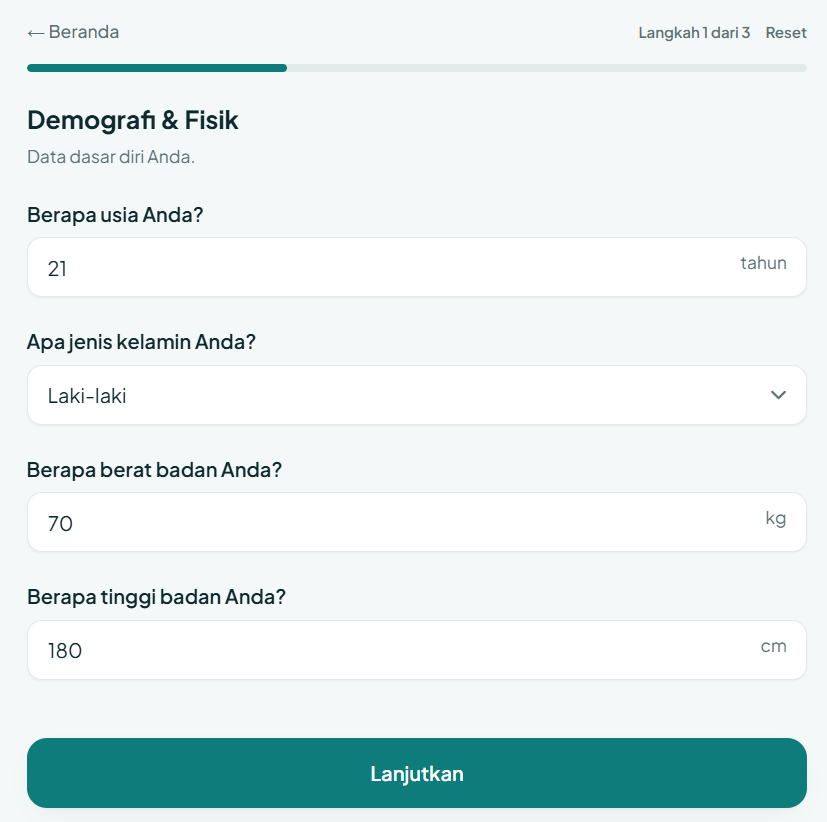
\includegraphics[width=0.65\textwidth]{images/prototype/form_input_1.png}
    \caption{Antarmuka pengisian data faktor risiko non-invasif (Langkah 1)}
    \label{fig:proto-form-1}
\end{figure}

\begin{figure}[H]
    \centering
    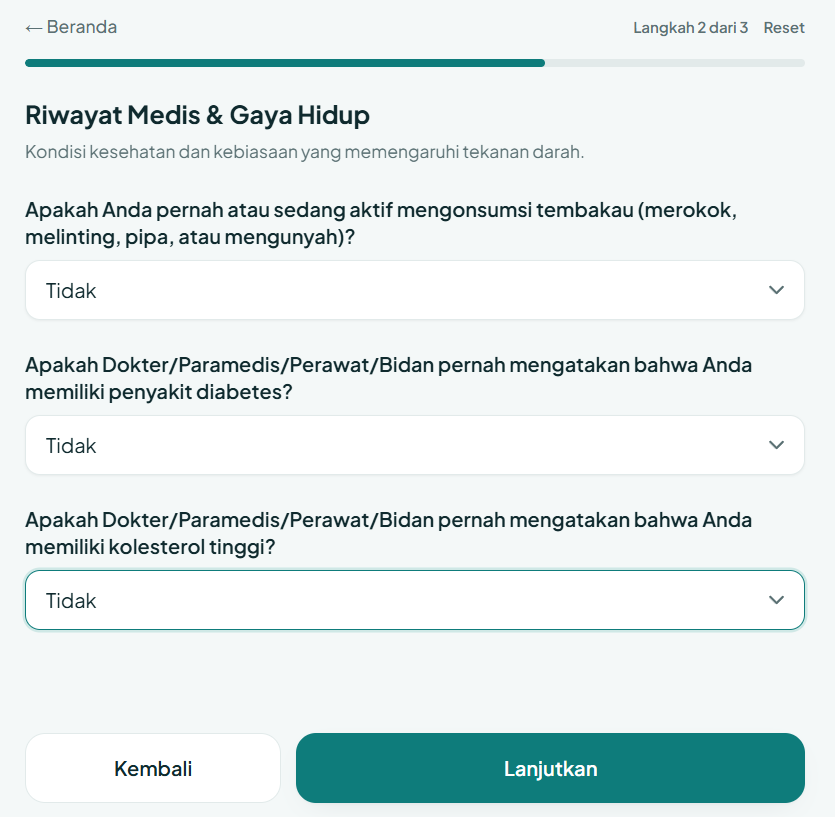
\includegraphics[width=0.65\textwidth]{images/prototype/form_input_2.png}
    \caption{Antarmuka pengisian data faktor risiko non-invasif (Langkah 2)}
    \label{fig:proto-form-2}
\end{figure}

\begin{figure}[H]
    \centering
    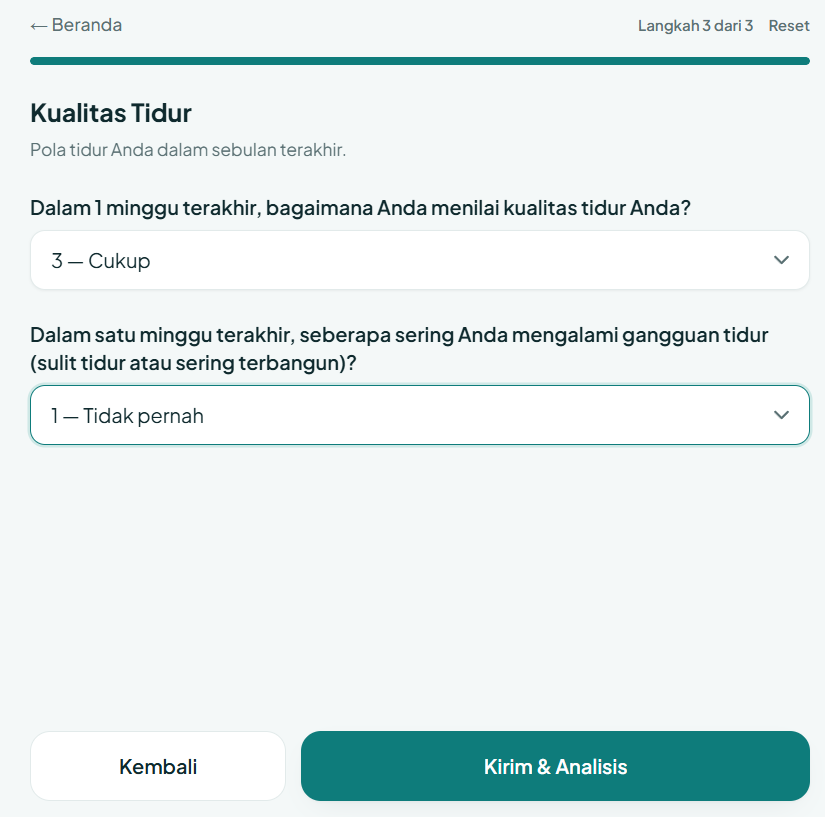
\includegraphics[width=0.65\textwidth]{images/prototype/form_input_3.png}
    \caption{Antarmuka pengisian data faktor risiko non-invasif (Langkah 3)}
    \label{fig:proto-form-3}
\end{figure}

Berat dan tinggi badan tidak dikirim langsung, melainkan dikonversi terlebih dahulu menjadi indeks massa tubuh (BMI) di sisi klien, sehingga backend menerima tepat delapan fitur sesuai urutan yang diharapkan model. Setelah pengguna melengkapi ketiga langkah, frontend mengirimkan kedelapan fitur ke \textit{endpoint} \textit{/api/v1/analyze}. Backend kemudian menghitung probabilitas melalui fungsi \textit{predict\_proba} pada model XGBoost, mengklasifikasikannya memakai ambang Youden, menghitung atribusi SHAP, lalu menyusun narasi melalui lapisan deterministik dan LLM. Seluruh hasil dikembalikan sebagai satu respons JSON yang langsung dirender pada halaman hasil.


\subsection{Keluaran Sistem}
Halaman hasil menyajikan tiga luaran secara terpadu untuk setiap analisis. Pertama, status risiko ditampilkan sebagai label ``Risiko Rendah'' atau ``Risiko Tinggi'' beserta skor probabilitas dalam bentuk pengukur (\emph{meter}) berwarna, dengan hijau menandakan risiko rendah dan merah menandakan risiko tinggi. Kedua, grafik kontribusi faktor menampilkan hasil SHAP sebagai diagram batang horizontal; warna merah menandakan faktor yang menaikkan risiko dan hijau menandakan faktor yang menurunkannya, sedangkan panjang batang merepresentasikan kontribusi relatif tiap faktor terhadap total. Grafik ini turut menampilkan nilai masukan pengguna pada tiap faktor serta keterangan bahwa nilai yang ditampilkan merupakan kontribusi relatif, bukan persentase risiko total. Ketiga, narasi klinis menyajikan ringkasan tingkat risiko, penjelasan tiga faktor teratas, dan paragraf saran gaya hidup, yang ditutup dengan pernyataan bahwa hasil merupakan informasi pendukung awal dan bukan pengganti diagnosis tenaga kesehatan.

Ketiga luaran tersebut merupakan perwujudan langsung dari mekanisme pengaman yang telah diuraikan pada Subbab~\ref{subsec:implementasi-narasi}, misalnya penanganan khusus faktor merokok serta aturan arah anjuran natrium, sehingga keterbatasan model tidak berubah menjadi misinformasi pada tampilan akhir yang diterima pengguna.

% Sisipkan tangkapan layar halaman hasil (status risiko + grafik SHAP + narasi) di sini,
% lalu hapus tanda komentar dan tambahkan \ref jika ingin dirujuk dari paragraf di atas.
\begin{figure}[H]
    \centering
    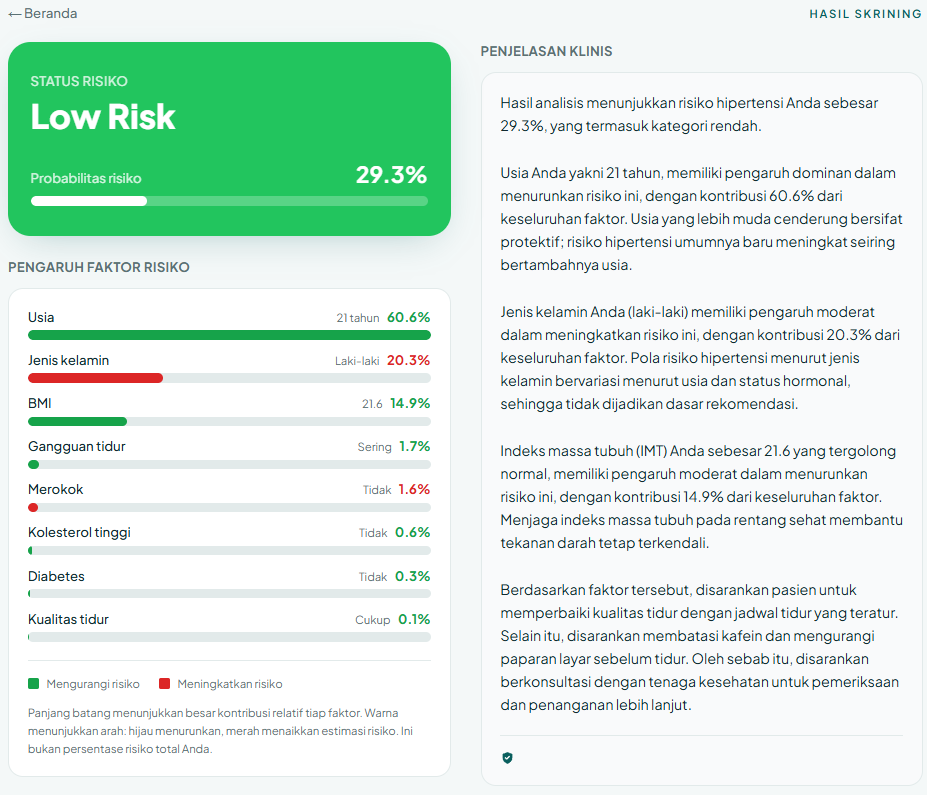
\includegraphics[width=0.8\textwidth]{images/hasil_prediksi.png}
    \caption{Halaman hasil: status risiko, grafik SHAP, dan narasi penjelasan}
    \label{fig:proto-hasil}
\end{figure}